\Opensolutionfile{ans}[ans/ansCD2D2-5.0]
\section{Phương trình - Bất phương trình mũ và logarit}
\begin{center}
	\textbf{CHUYÊN ĐỀ 1: PHƯƠNG TRÌNH MŨ}
\end{center}
\subsection{Kiến thức sách giáo khoa cần cần nắm}
\subsubsection{Phương trình mũ cơ bản $a^x=b\left(a>0, a\neq 1\right)$.}
\begin{itemize}
	\item Phương trình có một nghiệm duy nhất $x=\log_ab$ khi $b>0$.
	\item Phương trình vô nghiệm khi $b\leq 0$.
\end{itemize}
\subsubsection{Biến đổi, quy về cùng cơ số}
$a^{f(x)}=a^{g(x)}\Leftrightarrow a=1$ hoặc $\heva{&0<a\neq 1\\&f(x)=g(x).}$ \\
\subsubsection{Đặt ẩn phụ}
$f\left[a^{g(x)}\right]=0,\,(0<a\neq 1)\Leftrightarrow\heva{&t=a^{g(x)}>0\\&f(t)=0.}$ \\
Ta thường gặp các dạng:
\begin{itemize}
	\item $m.a^{2f(x)}+n\cdot a^{f(x)}+p=0$.
	\item $m.a^{f(x)}+n\cdot b^{f(x)}+p=0$, trong đó $a.b=1$. Đặt $t=a^{f(x)}(t>0)$, suy ra $b^{f(x)}=\dfrac{1}{t}$.
	\item $m.a^{2f(x)}+n\cdot (a\cdot b)^{f(x)}+p\cdot b^{2f(x)}=0$. Chia hai vế cho $b^{2f(x)}$ và đặt $t=\left(\dfrac{a}{b}\right)^{f(x)}>0$.
\end{itemize}
\subsubsection{Logarit hóa}
\begin{itemize}
	\item Phương trình $a^{f(x)}=b\Leftrightarrow\heva{&0<a\neq 1, b>0\\&f(x)=\log_ab.}$
	\item Phương trình $a^{f(x)}=b^{g(x)}\Leftrightarrow\log_aa^{f(x)}=\log_ab^{g(x)}\Leftrightarrow f(x)=g(x)\cdot\log_ab$.\\
	hoặc $\log_ba^{f(x)}=\log_bb^{g(x)}\Leftrightarrow f(x)\cdot\log_ba=g(x)$.
\end{itemize}
% \subsubsection{Sử dụng tính đơn điệu của hàm số}
% \begin{itemize}
% 	\item Tính chất 1. Nếu hàm số $y=f(x)$ luôn đồng biến (hoặc luôn nghịch biến) trên $(a;b)$ thì số nghiệm của phương trình $f(x)=k$ trên $(a;b)$ không nhiều hơn một và\\
% 	\[ f(u)=f(v)\Leftrightarrow u=v,\forall u,v\in(a;b). \]
% 	\item Tính chất 2. Nếu hàm số $y=f(x)$ liên tục và luôn đồng biến (hoặc luôn nghịch biến) trên $D$; hàm số $y=g(x)$ liên tục và luôn nghịch biến (hoặc luôn đồng biến) trên $D$ thì số nghiệm trên $D$ của phương trình $f(x)=g(x)$ không nhiều hơn một.
% \end{itemize}
\subsection{Phân loại và phương pháp giải bài tập}
\begin{dang}{Phương trình mũ cơ bản}
	\textbf{Phương pháp:} $a^{f(x)}=b$.\\
	Nếu $b<0$ thì phương trình vô nghiệm.\\
	Nếu $b>0$ thì phương trình có nghiệm duy nhất $f(x)=\log_ab$.
\end{dang}

\subsubsection{Các ví dụ}
\begin{vd}%[2D2Y5-1]%Ví dụ 1.
	Giải phương trình: $2^{2x-1}=3$.
	\loigiai{
	$2^{2x-1}=3\Leftrightarrow 2x-1=\log_23\Leftrightarrow x=\dfrac{\log_23+1}{2}$.}
\end{vd}

\begin{vd}%[2D2Y5-1]%Ví dụ 2.
	Giải phương trình: $\left(\dfrac{1}{2}\right)^{x^2-3x+1}=2$.
	\loigiai{
	$\left(\dfrac{1}{2}\right)^{x^2-3x+1}=2\Leftrightarrow x^2-3x+1=\log_{\tfrac{1}{2}}2\Leftrightarrow x^2-3x+1=-1\Leftrightarrow x^2-3x+2=0\Leftrightarrow\hoac{&x=1\\&x=2.}$}
\end{vd}

\begin{vd}%[2D2B5-1]%Ví dụ 3.
	Giải phương trình: $2^{x^2+3x-2}=\dfrac{1}{4}$.
	\loigiai{
	$2^{x^2+3x-2}=\dfrac{1}{4}\Leftrightarrow x^2+3x-2=\log_2\dfrac{1}{4}$ $ \Leftrightarrow x^2+3x-2=-2\Leftrightarrow x^2+3x=0\Leftrightarrow\hoac{&x=0\\&x=-3.} $ \\
	Vậy phương trình có nghiệm: $x=0,x=-3$.}
\end{vd}

\begin{vd}%[2D2B5-1]%Ví dụ 4.
	Giải phương trình sau: $5^x\cdot 2^{2x-1}=50$.
	\loigiai{
		$5^x\cdot 2^{2x-1}=50\Leftrightarrow 5^x\cdot\dfrac{4^x}{2}=50\Leftrightarrow 20^x=100\Leftrightarrow x=\log_{20}100$.\\
		Vậy phương trình có nghiệm: $x=\log_{20}100$.}
\end{vd}

\subsubsection{Câu hỏi trắc nghiệm}
\begin{ex}%[2D2B5-1]%Câu 1.
	Tính tổng tất cả các nghiệm thực của phương trình $2^{2x^2-7x+5}=1$. 
	\choice
	{$\dfrac{2}{7}$}
	{$\dfrac{5}{2}$}
	{$\dfrac{2}{5}$}
	{\True $\dfrac{7}{2}$}
	\loigiai{
	$2^{2x^2-7x+5}=1\Leftrightarrow 2x^2-7x+5=0\Leftrightarrow\hoac{&x=1\\&x=\dfrac{5}{2}}$.}
\end{ex}

\begin{ex}%[2D2B5-1]%Câu 2.
	Tìm tập nghiệm S của phương trình $3^{x^2-3x+4}=9$.
	\choice
	{$S=\{-2,1\}$}
	{$S=\{-1,3\}$}
	{\True $S=\{1,2\}$}
	{$S=\{1,3\}$}
	\loigiai{
	$3^{x^2-3x+4}=9\Leftrightarrow 3^{x^2-3x+4}=3^2\Leftrightarrow x^2-3x+4=2\Leftrightarrow x^2-3x+2=0\Leftrightarrow\hoac{&x=1\\&x=2}$.}
\end{ex}

\begin{ex}%[2D2B5-1]%Câu 3.
	Phương trình $(2+\sqrt{3})^{x^2-2x-2}=7-4\sqrt{3}$ có hai nghiệm $x_1,x_2$. Tính $P=x_1+x_2$. 
	\choice
	{$P=-1$}
	{$P=4$}
	{$P=3$}
	{\True $P=2$}
	\loigiai{
	$(2+\sqrt{3})^{x^2-2x-2}=7-4\sqrt{3}=(2-\sqrt{3})^2=(2+\sqrt{3})^{-2}\Leftrightarrow x^2-2x-2=-2\Leftrightarrow x^2-2x=0\Leftrightarrow\hoac{&x=0\\&x=2.}$}
\end{ex}

\begin{ex}%[2D2B5-1]%Câu 4.
	Tìm nghiệm của phương trình $2^{x+1}\cdot 5^x=200$. 
	\choice
	{$x=3$}
	{$x=\log_25$}
	{\True $x=2$}
	{$x=\log_52$}
	\loigiai{
	$2^{x+1}\cdot 5^x=200\Leftrightarrow 2\cdot 2^x\cdot 5^x=200\Leftrightarrow 10^x=10^2\Leftrightarrow x=2$.}
\end{ex}

\begin{ex}%[2D2B5-1]%Câu 5.
	Nghiệm của phương trình $3^{2x-1}=243$ là 
	\choice
	{$x=1$}
	{\True $x=3$}
	{$x=7$}
	{$x=2$}
	\loigiai{
	Cách 1: $3^{2x-1}=243\Leftrightarrow 3^{2x-1}=3^5\Leftrightarrow 2x-1=5\Leftrightarrow x=3$.\\
	Cách 2: Học sinh có thể thay từng giá trị $x$ ở đáp án vào phương trình. Giá trị nào thoả mãn thì lấy.\\
	Để cho tiện, học sinh dùng chức năng $CALC$ trong máy tính: Nhập $3^{2x-1}$ rồi $CALC$ từng giá trị. Giá trị nào bằng $243$ thì thoả mãn.}
\end{ex}

\begin{ex}%[2D2B5-1]%Câu 6.
	Gọi $x_1,x_2$ là nghiệm của phương trình $8^{x^2+6x-3}=4096,$ giá trị của $x_1\cdot x_2$ là bao nhiêu?
	\choice
	{$7$}
	{$9$}
	{$-9$}
	{\True $-7$}
	\loigiai{
	$8^{x^2+6x-3}=4096\Leftrightarrow x^2+6x-3=\log_84096=4\Leftrightarrow\hoac{&x=-7\\&x=1}$ \\
	$\Rightarrow p=x_1x_2=-7$.}
\end{ex}

\begin{ex}%[2D2K5-1]%Câu 7.
	Biết phương trình $9^x-2^{x+\dfrac{1}{2}}=2^{x+\dfrac{3}{2}}-3^{2x-1}$ có nghiệm là $a$. Khi đó biểu thức $a+\dfrac{1}{2}\log_{\tfrac{9}{2}}2$ có giá trị bằng
	\choice
	{$1-\dfrac{1}{2}\log_{\tfrac{9}{2}}2$}
	{\True $1$}
	{$1-\log_{\tfrac{9}{2}}2$}
	{$\dfrac{1}{2}\log_{\tfrac{9}{2}}2$}
	\loigiai{
		Ta có $9^x-2^{x+\dfrac{1}{2}}=2^{x+\dfrac{3}{2}}-3^{2x-1}\Leftrightarrow\dfrac{4}{3}\cdot 9^x=3\sqrt{2}\cdot 2^x\Leftrightarrow\left(\dfrac{9}{2}\right)^x=\dfrac{9}{2\sqrt{2}}\Leftrightarrow x=\log_{\tfrac{9}{2}}\dfrac{9}{2\sqrt{2}}$.\\
		Suy ra $a+\dfrac{1}{2}\log_{\tfrac{9}{2}}2=\log_{\tfrac{9}{2}}\dfrac{9}{2}=1$.}
\end{ex}

\begin{ex}%[2D2B5-1]%[THPT Bùi Thị Xuân - TP.HCM - Thi HKI (2016 - 2017)] %Câu 8.
	Tập hợp nghiệm của phương trình $3^{x^2-x-4}=\dfrac{1}{81}$ là
	\choice
	{$\{0;4\}$}
	{$\emptyset$}
	{$\{2;1\}$}
	{\True $\{0;1\}$}
	\loigiai{
		$3^{x^2-x-4}=\dfrac{1}{81}\Leftrightarrow 3^{x^2-x-4}=3^{-4}\Leftrightarrow x^2-x-4=-4\Leftrightarrow x^2-x=0\Leftrightarrow\hoac{&x=0\\&x=1.}$}
\end{ex}

\begin{ex}%[2D2B5-1]%[ChuyênNguyễnHuệ-HàNội-ThiHKI(2016-2017)]%Câu 9.
	Phương trình $3^{x^2-5}-81=0$ có hai nghiệm $x_1;x_2$. Tính giá trị của tích $x_1x_2$ 
	\choice
	{\True $-9$}
	{$9$}
	{$29$}
	{$-27$}
	\loigiai{
	$3^{x^2-5}-81=0\Leftrightarrow 3^{x^2-5}=3^4\Leftrightarrow x^2-5=4\Leftrightarrow\hoac{&x=3\\&x=-3.}$ \\
	Vậy tích $x_1x_2=-9$.}
\end{ex}

\begin{ex}%[2D2B5-1]%Câu 10.
	Cho phương trình $3^{x^2-4x+5}=9$ tổng lập phương các nghiệm thực của phương trình là 
	\choice
	{\True 28}
	{27}
	{26}
	{25}
	\loigiai{
	Ta có: $3^{x^2-4x+5}=9\Leftrightarrow 3^{x^2-4x+5}=3^2\Leftrightarrow x^2-4x+5=2\Leftrightarrow x^2-4x+3=0\Leftrightarrow\hoac{&x=1\\&x=3.}$ \\
	Suy ra $1^3+3^3=28$.}
\end{ex}

\begin{ex}%[2D2B5-1]%Câu 11.
	Tính tổng $T$ tất cả các nghiệm của phương trình $(x-3)^{2x^2-5x}=1$. 
	\choice
	{$T=0$}
	{$T=4$}
	{\True $T=\dfrac{13}{2}$}
	{$T=\dfrac{15}{2}$}
	\loigiai{
	Ta xét các trường hợp sau:\\
	TH1. $x-3=1\Leftrightarrow x=4$ thỏa mãn phương trình.\\
	TH2. $\heva{&x-3\neq 0\\&2x^2-5x=0}\Leftrightarrow\hoac{&x=0\\&x=\dfrac{5}{2}.}$ \\
	Vậy phương trình đã cho có ba nghiệm $x=0; x=\dfrac{5}{2}; x=4\Rightarrow T=\dfrac{13}{2}$.}
\end{ex}

\begin{dang}{Phương pháp đưa về cơ số}
	\textbf{Phương pháp:} Biến đổi phương trình về dạng: $a^{f(x)}=a^{g(x)} \quad (1)$.\\
	+ Nếu cơ số $a$ là một số dương và khác $1$ thì: $(1)\Leftrightarrow f(x)=g(x)$.\\
	+ Nếu cơ số $a$ thay đổi thì: $(1)\Leftrightarrow\heva{&a>0\\&(a-1)[f(x)-g(x)]=0.}$
\end{dang}

\subsubsection{Các ví dụ}
\begin{vd}%[2D2B5-2]%Ví dụ 1.
	Giải phương trình sau: $2^{x^2-x+8}=4^{1-3x}$.
	\loigiai{
	\begin{eqnarray*}
	&&2^{x^2-x+8}=4^{1-3x}\Leftrightarrow 2^{x^2-x+8}=(2^2)^{1-3x}\\
	&\Leftrightarrow& 2^{x^2-x+8}=2^{2\cdot (1-3x)}\Leftrightarrow 2^{x^2-x+8}=2^{2-6x}\\
	&\Leftrightarrow& x^2-x+8=2-6x\Leftrightarrow\hoac{&x=-2\\&x=-3.}
	\end{eqnarray*}
	}
\end{vd}

\begin{vd}%[2D2B5-2]%Ví dụ 2.
	Giải phương trình sau: $2^{x^2-6x-\dfrac{5}{2}}=16\sqrt{2}$.
	\loigiai{
	\begin{eqnarray*}
	&&2^{x^2-6x-\dfrac{5}{2}}=16\sqrt{2}\Leftrightarrow 2^{x^2-6x-\dfrac{5}{2}}=2^{\tfrac{9}{2}}\\
	&\Leftrightarrow &x^2-6x-\dfrac{5}{2}=\dfrac{9}{2}\Leftrightarrow\hoac{&x=-1\\&x=7.}
	\end{eqnarray*}
	}
\end{vd}

\begin{vd}%[2D2B5-2]%Ví dụ 3.
	Giải phương trình sau: $2^{x+1}+2^{x-2}=36$.
	\loigiai{
	\begin{eqnarray*}
	&&2^{x+1}+2^{x-2}=36\Leftrightarrow 2\cdot 2^x+\dfrac{2^x}{4}=36 \\
	&\Leftrightarrow& \dfrac{{8\cdot 2}^x+2^x}{4}=36 \Leftrightarrow 9\cdot 2^x=36\cdot 4\\
	&\Leftrightarrow& 2^x=16 \Leftrightarrow 2^x=2^4\Leftrightarrow x=4.
	\end{eqnarray*}
	Vậy phương trình có nghiệm: $x=1,x=2$.}
\end{vd}

\begin{vd}%[2D2B5-2]%Ví dụ 4.
	Giải phương trình sau: $2.3^{x+1}-6\cdot 3^{x-1}-3^x=9$.
	\loigiai{
	\begin{eqnarray*}
	2.3^{x+1}-6\cdot 3^{x-1}-3^x=9 &\Leftrightarrow& 6\cdot 3^x-2\cdot 3^x-3^x=9\\
	&\Leftrightarrow& 3\cdot 3^x=9\Leftrightarrow 3^x=3\Leftrightarrow x=1.
	\end{eqnarray*}
	}
\end{vd}

\begin{vd}%[2D2B5-2]%Ví dụ 5.
	Giải phương trình sau: $2^{x^2-6} \cdot 3^{x^2-6} =\dfrac{1}{6^5} \cdot\left(6^{x-1} \right)^4$.
	\loigiai{
	\begin{eqnarray*}
	&&2^{x^2-6}3^{x^2-6}=\dfrac{1}{6^5}\cdot\left(6^{x-1}\right)^4\Leftrightarrow(2\cdot 3)^{x^2-6}=\dfrac{6^{4x-4}}{5}\\
	&\Leftrightarrow& 6^{x^2-6}=6^{4x-9}\Leftrightarrow x^2-6=4x-9\\
	&\Leftrightarrow& x^2-4x+3=0\Leftrightarrow\hoac{&x=1\\&x=3.}
	\end{eqnarray*}
	}
\end{vd}

\begin{vd}%[2D2B5-2]%Ví dụ 6.
	Giải phương trình sau: $2^{x^2-1}-3^{x^2}=3^{x^2-1}-2^{x^2+2}$.
	\loigiai{
	\begin{eqnarray*}
	&&2^{x^2-1}-3^{x^2}=3^{x^2-1}-2^{x^2+2}\Leftrightarrow\dfrac{2^{x^2}}{2}-3^{x^2}=\dfrac{3^{x^2}}{3}-4\cdot 2^{x^2}\\
	&\Leftrightarrow& 2^{x^2}\cdot\left(\dfrac{1}{2}+4\right)=3^{x^2}\cdot\left(\dfrac{1}{3}+1\right)\Leftrightarrow 2^{x^2}\cdot\dfrac{9}{2}=3^{x^2}\cdot\left(\dfrac{4}{3}\right)\\
	&\Leftrightarrow& \left(\dfrac{2}{3}\right)^{x^2}=\left(\dfrac{2}{3}\right)^3\Leftrightarrow x^2=3\Leftrightarrow x=\pm\sqrt{3}.
	\end{eqnarray*}
	}
\end{vd}

\subsubsection{Câu hỏi trắc nghiệm}
\begin{ex}%[2D2B5-2]%Câu 1.
	Tìm nghiệm của phương trình $3^{x-4}=\left(\dfrac{1}{9}\right)^{3x-1}$ 
	\choice
	{$\dfrac{1}{3}$}
	{$1$}
	{\True $\dfrac{6}{7}$}
	{$\dfrac{7}{6}$}
	\loigiai{
	\begin{eqnarray*}
	&&3^{x-4}=\left(\dfrac{1}{9}\right)^{3x-1}=3^{-2(3x-1)}\\
	&\Leftrightarrow& x-4=-2(3x-1)\\
	&\Leftrightarrow& 7x=6\Leftrightarrow x=\dfrac{6}{7}.
	\end{eqnarray*}
	}
\end{ex}

\begin{ex}%[2D2B5-2]%Câu 2.
	Tìm nghiệm của phương trình $\left(\dfrac{1}{25}\right)^{x+1}=125^{2x}$. 
	\choice
	{$1$}
	{$4$}
	{\True $-\dfrac{1}{4}$}
	{$-\dfrac{1}{8}$}
	\loigiai{
	\begin{eqnarray*}
	&&\left(\dfrac{1}{25}\right)^{x+1}=125^{2x}\Leftrightarrow 5^{-2(x+1)}=5^{6x}\\
	&\Leftrightarrow& -2(x+1)=6x\Leftrightarrow 4x=-1\Leftrightarrow x=-\dfrac{1}{4}.
	\end{eqnarray*}
	}
\end{ex}

\begin{ex}%[2D2K5-2]%Câu 3.
	Tìm nghiệm của phương trình $8^{\tfrac{2x-1}{x+1}}=0,25\cdot (\sqrt{2})^x$. 
	\choice
	{\True $x=\dfrac{15\pm\sqrt{217}}{2}$}
	{$x=\dfrac{17\pm\sqrt{215}}{2}$}
	{$x=15\pm\sqrt{217}$}
	{$x=17\pm\sqrt{215}$}
	\loigiai{
	\begin{eqnarray*}
	&&8^{\tfrac{2x-1}{x+1}}=0,25\cdot (\sqrt{2})^x\Leftrightarrow 2^{\tfrac{3(2x-1)}{x+1}}=2^{-2}\cdot 2^{\tfrac{x}{2}}\\
	&\Leftrightarrow& 2^{\tfrac{3(2x-1)}{x+1}}=2^{\tfrac{x-4}{2}}\Leftrightarrow\dfrac{3(2x-1)}{x+1}=\dfrac{x-4}{2}\\
	&\Leftrightarrow& 6(2x-1)=(x+1)(x-4)\Leftrightarrow x^2-15x+2=0\Leftrightarrow x=\dfrac{15\pm\sqrt{217}}{2}.
	\end{eqnarray*}
	}
\end{ex}

\begin{ex}%[2D2K5-2]%Câu 4.
	Tìm nghiệm của phương trình $\dfrac{3^{2x-6}}{27}=\dfrac{1}{3^x}$. 
	\choice
	{$x=5$}
	{$x=4$}
	{\True $x=3$}
	{$x=2$}
	\loigiai{
	\textbf{Cách 1:} $\dfrac{3^{2x-6}}{27}=\dfrac{1}{3^x}\Leftrightarrow 3^{2x-9}=3^{-x}\Leftrightarrow 2x-9=-x\Leftrightarrow x=3$.\\
	\textbf{Cách 2:} Lần lượt thử các phương án vào phương trình đã cho, ta thấy $x=3$ thỏa mãn.}
\end{ex}

\begin{ex}%[2D2K5-2]%Câu 5.
	Tìm nghiệm của phương trình $2^x=(\sqrt{3})^x$. 
	\choice
	{$x=3$}
	{$x=5$}
	{$x=-1$}
	{\True $x=0$}
	\loigiai{
	\textbf{Cách 1:} $2^x=(\sqrt{3})^x\Leftrightarrow\left(\dfrac{2}{\sqrt{3}}\right)^x=1\Leftrightarrow x=0$.\\
	\textbf{Cách 2:} Lần lượt thử các phương án vào phương trình đã cho, ta thấy $x=0$ thỏa mãn.
	}
\end{ex}

\begin{ex}%[2D2K5-2]%Câu 6.
	Tìm nghiệm của phương trình $(\sqrt{2}-1)^{x^2}=(\sqrt{2}+1)^{2x+1}$. 
	\choice
	{\True $x=-1$}
	{$x=1$}
	{$x=-2$}
	{$x=2$}
	\loigiai{
	\textbf{Cách 1:} 
	\begin{eqnarray*}
	&&(\sqrt{2}-1)^{x^2}=(\sqrt{2}+1)^{2x+1}=(\sqrt{2}-1)^{-(2x+1)}\\
	&\Leftrightarrow& x^2=-(2x+1)\Leftrightarrow (x+1)^2=0\Leftrightarrow x=-1.
	\end{eqnarray*}
	\textbf{Cách 2:} Lần lượt thử các phương án vào phương trình đã cho, ta thấy $x=-1$ thỏa mãn.}
	\end{ex}

\begin{ex}%[2D2K5-2]%Câu 7.
	Tìm nghiệm của phương trình $2^x+2^{x+1}+2^{x+2}=21$. 
	\choice
	{$x=\log_32$}
	{\True $x=\log_23$}
	{$x=2$}
	{$x=3$}
	\loigiai{
	\begin{eqnarray*}
	&&2^x+2^{x+1}+2^{x+2}=21\Leftrightarrow 2^x+2\cdot 2^x+4\cdot 2^x=21\\
	&\Leftrightarrow& 7\cdot 2^x=21\Leftrightarrow 2^x=3\Leftrightarrow x=\log_23.
	\end{eqnarray*}
	}
\end{ex}

\begin{ex}%[2D2K5-2]%Câu 8.
	Tìm nghiệm của phương trình $\dfrac{{2\cdot 3}^x-2^{x+2}}{3^x-2^x}=1$. 
	\choice
	{$x=\log_{\tfrac{2}{3}}3$}
	{$x=\log_{\tfrac{2}{3}}2$}
	{\True $x=\log_{\tfrac{3}{2}}3$}
	{$x=1$}
	\loigiai{
	\begin{eqnarray*}
	&&\dfrac{{2\cdot 3}^x-2^{x+2}}{3^x-2^x}=1,\,(x\neq 0)\Leftrightarrow 2\cdot 3^x-2^{x+2}=3^x-2^x\\
	&\Leftrightarrow& 2\cdot 3^x-4\cdot 2^x=3^x-2^x\Leftrightarrow 3^x=3\cdot 2^x \Leftrightarrow\left(\dfrac{3}{2}\right)^x=3\Leftrightarrow x=\log_{\tfrac{3}{2}}3.
	\end{eqnarray*}
		}
\end{ex}

\begin{ex}%[2D2K5-2]%Câu 9.
	Nghiệm của phương trình $\left(\dfrac{2}{3}\right)^{2x-1}=\left(\dfrac{9}{4}\right)^{2x+3}$ là 
	\choice
	{\True $x=-\dfrac{5}{6}$}
	{$x=\dfrac{2}{3}$}
	{$x=3$}
	{$x=\dfrac{5}{2}$}
	\loigiai{
	\begin{eqnarray*}
	&&\left(\dfrac{2}{3}\right)^{2x-1}=\left(\dfrac{9}{4}\right)^{2x+3}\Leftrightarrow\left(\dfrac{2}{3}\right)^{2x-1}=\left(\dfrac{2}{3}\right)^{-4x-6}\\
	&\Leftrightarrow& 2x-1=-4x-6\Leftrightarrow x=-\dfrac{5}{6}.
	\end{eqnarray*}
	}
\end{ex}

\begin{ex}%[2D2B5-2]%Câu 10.
	Phương trình $0,125\cdot 4^{x+4}=\left(\dfrac{\sqrt{2}}{4}\right)^{-4x+2}$ có nghiệm là 
	\choice
	{\True $x=2$}
	{$x=1$}
	{$x=-2$}
	{$x=-1$}
	\loigiai{
	\begin{eqnarray*}
	&&0,125\cdot 4^{x+4}=\left(\dfrac{\sqrt{2}}{4}\right)^{-4x+2}\Leftrightarrow\dfrac{1}{8}\cdot 2^{2x+8}=\dfrac{2^{-2x+1}}{2^{-8x+4}}\\
	&\Leftrightarrow& 2^{2x+5}=2^{6x-3}	\Leftrightarrow 2x+5=6x-3\Leftrightarrow x=2.
	\end{eqnarray*}
	}
\end{ex}

\begin{dang}{Phương pháp đặt ẩn phụ}
	\textbf{Phương pháp:} $f\left[a^{g(x)}\right]=0,\,(0<a\neq 1) \Leftrightarrow \heva{&t=a^{g(x)}>0\\&f(t)=0.}$ \\
	Ta thường gặp các dạng:
	\begin{itemize}
		\item $m.a^{2f(x)}+n\cdot a^{f(x)}+p=0$.
		\item $m.a^{f(x)}+n\cdot b^{f(x)}+p=0$, trong đó $a.b=1$. Đặt $t=a^{f(x)}(t>0)$, suy ra $b^{f(x)}=\dfrac{1}{t}$.
		\item $m.a^{2f(x)}+n\cdot (a\cdot b)^{f(x)}+p\cdot b^{2f(x)}=0$. Chia hai vế cho $b^{2f(x)}$ và đặt $t=\left(\dfrac{a}{b}\right)^{f(x)}>0$.
	\end{itemize}
\end{dang}

\subsubsection{Các ví dụ}
\begin{vd}%[2D2K5-3]%Ví dụ 1.
	Giải các phương trình sau: $3^{2x+8}-4\cdot 3^{x+5}+27=0$.
	\loigiai{
	$3^8\cdot 3^{2x}-4\cdot 3^5\cdot 3^x+27=0$ \\
	$ \Leftrightarrow 6561\cdot (3^x)^2-972\cdot 3^x+27=0 $ \quad (*).\\
	Đặt $t=3^x>0$ (các em có thể đặt t = 3x+4).\\
	Phương trình (*) $\Leftrightarrow 6561t^2-972t+27=0\Leftrightarrow\hoac{&t=\dfrac{1}{9}\\&t=\dfrac{1}{27}.}$ \\
	Với $t=\dfrac{1}{9}\Leftrightarrow 3^x=3^{-2}\Leftrightarrow x=-2$.\\
	Với $t=\dfrac{1}{27}\Leftrightarrow 3^x=3^{-3}\Leftrightarrow x=-3$.\\
	Vậy phương trình có nghiệm: $x=-2,x=-3$.}
\end{vd}

\begin{vd}%[2D2B5-3]%Ví dụ 2.
	Giải các phương trình sau: $25^x-2\cdot 5^x-15=0$.
	\loigiai{
		$25^x-2\cdot 5^x-15=0\Leftrightarrow(5^x)^2-2\cdot 5^x-15=0$ \quad (*).\\
		Đặt $t=5^x>0$.\\
		Phương trình (*) $\Leftrightarrow t^2-2t-15=0\Leftrightarrow\hoac{&t=5\\&t=-3 \text{ (loại)}.}$ \\
		Với $t=5\Leftrightarrow 5^x=5\Leftrightarrow x=1$.\\
		Vậy phương trình có nghiệm: $x=1$.}
\end{vd}

\begin{vd}%[2D2K5-3]%Ví dụ 3.
	Giải các phương trình sau: $3^{x+2}-3^{2-x}=24$.
	\loigiai{
		$3^{x+2}-3^{2-x}=24\Leftrightarrow 9\cdot 3^x-\dfrac{9}{3^x}-24=0\Leftrightarrow 9\cdot (3^x)^2-24\cdot 3^x-9=0$ \quad (*).\\
		Đặt $t=3^x>0$.\\
		(*) $\Leftrightarrow 9t^2-24t-9=0\Leftrightarrow\hoac{&t=3\\&t=-\dfrac{1}{3} \text{ (loại)}.}$ \\
		Với $t=3\Leftrightarrow 3^x=3\Leftrightarrow x=1$.\\
		Vậy phương trình có nghiệm: $x=1$.}
\end{vd}

\begin{vd}%[2D2K5-3]%Ví dụ 4.
	Giải phương trình sau:
	\begin{enumerate}[a)]
		\item  $6.9^x-13\cdot 6^x+6\cdot 4^x=0$.
		\item $2.2^{2x}-9\cdot 14^x+7\cdot 7^{2x}=0$.
		\item $25^x+10^x=2^{2x+1}$.
	\end{enumerate}
	\loigiai{
	\begin{enumerate}[a)]
		\item $6.9^x-13\cdot 6^x+6\cdot 4^x=0\Leftrightarrow 6\cdot\left(\dfrac{3}{2}\right)^{2x}-13\cdot\left(\dfrac{3}{2}\right)^x+6=0\Leftrightarrow\heva{&\left(\dfrac{3}{2}\right)^x=\dfrac{3}{2}\\&\left(\dfrac{3}{2}\right)^x=\dfrac{2}{3}}\Leftrightarrow\heva{&x=1\\&x=-1.}$
		\item $2.2^{2x}-9\cdot 14^x+7\cdot 7^{2x}=0\Leftrightarrow 2-9\left(\dfrac{7}{2}\right)^x+7\cdot\left(\dfrac{7}{2}\right)^{2x}=0\Leftrightarrow\hoac{&\left(\dfrac{7}{2}\right)^x=1\\&\left(\dfrac{7}{2}\right)^x=\dfrac{2}{7}}\Leftrightarrow\hoac{&x=0\\&x=-1.}$
		\item $25^x+10^x=2^{2x+1}\Leftrightarrow 25^x+10^x-2\cdot 4^x=0\Leftrightarrow\left(\dfrac{5}{2}\right)^{2x}+\left(\dfrac{5}{2}\right)^x-2=0\Leftrightarrow\heva{&\left(\dfrac{5}{2}\right)^x=1\\&\left(\dfrac{5}{2}\right)^x=-2(l)}\Leftrightarrow x=0$.
	\end{enumerate}
	}
\end{vd}

\begin{vd}%[2D2K5-3]%Ví dụ 5.
	Giải phương trình sau: $(2+\sqrt{3})^x+(2-\sqrt{3})^x=4$.
	\loigiai{
	Để ý: $(2+\sqrt{3})\cdot (2-\sqrt{3})=1$.\\
	Đặt $t=(2+\sqrt{3}),t>0\Rightarrow(2-\sqrt{3})^x=\left(\dfrac{1}{2+\sqrt{3}}\right)^x=\dfrac{1}{(2+\sqrt{3})^x}=\dfrac{1}{t}$.\\
	Ta có: $t+\dfrac{1}{t}=4\Leftrightarrow t^2-4t+1=0\Leftrightarrow\hoac{&t=2+\sqrt{3}\\&t=2-\sqrt{3}}\Rightarrow\heva{&(2+\sqrt{3})^x=2+\sqrt{3}\\&(2+\sqrt{3})^x=2-\sqrt{3}}\Leftrightarrow\heva{&x=1\\&x=-1.}$}
\end{vd}

\subsubsection{Câu hỏi trắc nghiệm}
\begin{ex}%[2D2B5-3]%Câu 1.
	Tìm nghiệm của phương trình $9^x-3\cdot 3^x+2=0$. 
	\choice
	{$\hoac{&x=0\\&x=\log_23}$}
	{\True $\hoac{&x=0\\&x=\log_32}$}
	{$\hoac{&x=0\\&x=-\log_23}$}
	{$\hoac{&x=0\\&x=-\log_32}$}
	\loigiai{
	$9^x-3\cdot 3^x+2=0\Leftrightarrow 3^{2x}-3\cdot 3^x+2=0\Leftrightarrow\hoac{&3^x=1\\&3^x=2}\Leftrightarrow\hoac{&x=0\\&x=\log_32.}$}
\end{ex}

\begin{ex}%[2D2B5-3]%Câu 2.
	Biết phương trình $4^x-2^{x+1}-3=0$ có duy nhất một nghiệm là $a$. Tính $P=a\log_34+1$. 
	\choice
	{$P=2$}
	{$P=4$}
	{\True $P=3$}
	{$P=5$}
	\loigiai{
	$4^x-2^{x+1}-3=0\Leftrightarrow 2^{2x}-2\cdot 2^x-3=0\Leftrightarrow\hoac{&2^x=-1\text{ (vô nghiệm)}\\&2^x=3} \Leftrightarrow x=\log_23$. \\
	$ \Rightarrow P=\log_23\cdot\log_34+1=\log_24+1=3 $.}
\end{ex}

\begin{ex}%[2D2B5-3]%Câu 3.
	Cho phương trình $4^x+2^{x+1}-3=0$. Khi đặt $t=2^x$, ta được phương trình nào dưới đây?
	\choice
	{$2t^2-3=0$}
	{$t^2+t-3=0$}
	{$4t-3=0$}
	{\True $t^2+2t-3=0$}
	\loigiai{
	$4^x+2^{x+1}-3=0\Leftrightarrow 2^{2x}+2\cdot 2^x-3=0$.}
\end{ex}

\begin{ex}%[2D2K5-3]%Câu 4.
	Tìm nghiệm của phương trình $\mathrm{e}^{6x}-3\cdot\mathrm{e}^{3x}+2=0$ 
	\choice
	{\True $\hoac{&x=0\\&x=\dfrac{1}{3}\ln 2}$}
	{$\hoac{&x=-1\\&x=\dfrac{1}{3}\ln 2}$}
	{$\hoac{&x=0\\&x=-1}$}
	{$\hoac{&x=0\\&x=1}$}
	\loigiai{
	$\mathrm{e}^{6x}-3\cdot\mathrm{e}^{3x}+2=0\Leftrightarrow\left(\mathrm{e}^{3x}\right)^2-3\cdot\mathrm{e}^{3x}+2=0\Leftrightarrow\hoac{&\mathrm{e}^{3x}=1\\&\mathrm{e}^{3x}=2}\Leftrightarrow\hoac{&3x=0\\&3x=\log_e2}\Leftrightarrow\hoac{&x=0\\&x=\dfrac{1}{3}\ln 2.}$}
\end{ex}

\begin{ex}%[2D2K5-3]%Câu 5.
	Số nghiệm của phương trình $7^{2x+1}-8\cdot 7^x+1=0$ là
	\choice
	{$0$}
	{\True $2$}
	{$1$}
	{$3$}
	\loigiai{
	$7^{2x+1}-8\cdot 7^x+1=0\Leftrightarrow 7\cdot 7^x-8\cdot 7^x+1=0\Leftrightarrow\hoac{&7^x=1\\&7^x=\dfrac{1}{7}=7^{-1}}\Leftrightarrow\hoac{&x=0\\&x=-1}$.}
\end{ex}

\begin{ex}%[2D2K5-3]%Câu 6.
	Gọi $x_1,x_2$ là hai nghiệm thực của phương trình $(2+\sqrt{3})^x+2(2-\sqrt{3})^x=3$.\\
	Tính $P=x_1+x_2$. 
	\choice
	{\True $P=\log_{2+\sqrt{3}}2$}
	{$P=0$}
	{$P=\log_{2-\sqrt{3}}2$}
	{$P=2$}
	\loigiai{
	Vì $(2+\sqrt{3})^x\cdot (2-\sqrt{3})^x=1$, nên ta đặt $(2+\sqrt{3})^x=t\Rightarrow(2-\sqrt{3})^x=\dfrac{1}{t}$.\\
	Thay vào phương trình ta được $t+2\cdot\dfrac{1}{t}=3\Leftrightarrow t^2-3t+2=0\Leftrightarrow\hoac{&t=1\\&t=2}$ \\
	$\Rightarrow\hoac{&(2+\sqrt{3})^x=1\\&(2+\sqrt{3})^x=2} \Leftrightarrow\hoac{&x=0\\&x=\log_{2+\sqrt{3}}2}\Rightarrow P=\log_{2+\sqrt{3}}2$.}
\end{ex}

\begin{ex}%[2D2K5-3]%Câu 7.
	Gọi $x_1,x_2$ là hai nghiệm thực của phương trình $\left(5-\sqrt{21}\right)^x+7\left(5+\sqrt{21}\right)^x=2^{x+3}$.\\
	Tính $P=x_1+x_2$. 
	\choice
	{$P=\log_{\tfrac{5+\sqrt{21}}{2}}7$}
	{$P=-8$}
	{$P=8$}
	{\True $P=\log_{\tfrac{5-\sqrt{21}}{2}}7$}
	\loigiai{
	\begin{eqnarray*}
	&&\left(5-\sqrt{21}\right)^x+7\left(5+\sqrt{21}\right)^x=2^{x+3}\\
	&\Leftrightarrow& \left(5-\sqrt{21}\right)^x+7\left(5+\sqrt{21}\right)^x=8\cdot 2^x\\
	&\Leftrightarrow& \left(\dfrac{5-\sqrt{21}}{2}\right)^x+7\left(\dfrac{5+\sqrt{21}}{2}\right)^x=8.
	\end{eqnarray*}
	Đặt $\left(\dfrac{5-\sqrt{21}}{2}\right)^x=t(t>0) \Rightarrow\left(\dfrac{5+\sqrt{21}}{2}\right)^x =\dfrac{1}{t}$.\\
	Thay vào phương trình, ta được $t+7\cdot\dfrac{1}{t}=8\Leftrightarrow t^2-8t+7=0\Leftrightarrow\hoac{&t=1\\&t=7}$ \\
	$ \Rightarrow \hoac{&\left(\dfrac{5-\sqrt{21}}{2}\right)^x=1\\&\left(\dfrac{5-\sqrt{21}}{2}\right)^x=7} \Leftrightarrow\hoac{&x=0\\&x=\log_{\tfrac{5-\sqrt{21}}{2}}7} \Rightarrow P=\log_{\tfrac{5-\sqrt{21}}{2}}7 $.}
\end{ex}

\begin{ex}%[2D2K5-3]%Câu 8.
	Số nghiệm của phương trình $6.9^{\tfrac{1}{x}}-13\cdot 6^{\tfrac{1}{x}}+6\cdot 4^{\tfrac{1}{x}}=0$ là 
	\choice
	{$3$}
	{\True $2$}
	{$1$}
	{$0$}
	\loigiai{
	\begin{eqnarray*}
	&&6.9^{\tfrac{1}{x}}-13\cdot 6^{\tfrac{1}{x}}+6\cdot 4^{\tfrac{1}{x}}=0,\,(x\neq 0)\\
	&\Leftrightarrow& 6\cdot\dfrac{9^{\tfrac{1}{x}}}{4^{\tfrac{1}{x}}}-13\cdot\dfrac{6^{\tfrac{1}{x}}}{4^{\tfrac{1}{x}}}+6=0\\
	&\Leftrightarrow& 6\cdot\left(\dfrac{3}{2}\right)^{2\cdot\dfrac{1}{x}}-13\cdot\left(\dfrac{3}{2}\right)^{\tfrac{1}{x}}+6=0.
	\end{eqnarray*}
	Đặt $\left(\dfrac{3}{2}\right)^{\tfrac{1}{x}}=t,\,(t>0)$.\\
	Thay vào phương trình ta được: $6t^2-13t+6=0\Leftrightarrow\hoac{&t=\dfrac{3}{2}\\&t=\dfrac{2}{3}.}$ \\
	Với 2 giá trị của $t$ thay vào $\left(\dfrac{3}{2}\right)^{\tfrac{1}{x}}=t$ ta được 2 giá trị của $x$.}
\end{ex}

\begin{ex}%[2D2K5-3]%Câu 9.
	Số nghiệm của phương trình $3.8^x+4\cdot 12^x-18^x-2\cdot 27^x=0$ là 
	\choice
	{\True $1$}
	{$2$}
	{$0$}
	{$3$}
	\loigiai{
	$3.8^x+4\cdot 12^x-18^x-2\cdot 27^x=0\Leftrightarrow 3+4\cdot\left(\dfrac{3}{2}\right)^x-\left(\dfrac{3}{2}\right)^{2x}-2\cdot\left(\dfrac{3}{2}\right)^{3x}=0$.\\
	Đặt $\left(\dfrac{3}{2}\right)^x=t,\,(t>0)$.\\
	Thay vào phương trình, ta được:\\
	$2t^3+t^2-4t-3=0\Leftrightarrow(t+1)\left(2t^2-t-3\right)=0\Leftrightarrow\hoac{&t=-1 \text{ (loại)} \\&t=\dfrac{3}{2}.}$ \\
	Với $t=\dfrac{3}{2}\Rightarrow\left(\dfrac{3}{2}\right)^x =\dfrac{3}{2}\Leftrightarrow x=1$.}
\end{ex}

\begin{ex}%[2D2K5-3]%Câu 10.
	Gọi $x_1,x_2$ là hai nghiệm của phương trình: $2^{2x^4+4x^2-6}-2\cdot 2^{x^4+2x^2-3}+1=0$.\\
	Tính $P=x_1\cdot x_2$. 
	\choice
	{$P=-9$}
	{\True $P=-1$}
	{$P=1$}
	{$P=9$}
	\loigiai{
	Đặt $2^{x^4+2x^2-3}=t,\,(t>0)$.\\
	Thay vào phương trình, ta được: $t^2-2t+1=0\Leftrightarrow t=1$.\\
	Với $t=1$, ta có: $2^{x^4+2x^2-3}=1\Leftrightarrow x^4+2x^2-3=0\Leftrightarrow x^2=1\Leftrightarrow x=\pm 1$ \\
	$ \Rightarrow P=(-1)\cdot 1=-1 $.}
\end{ex}

\begin{ex}%[2D2K5-3]%Câu 11.
	Tìm nghiệm của phương trình $2.2^{\sin^2x}-2^{\cos^2x}-3=0$. 
	\choice
	{$x=(2k+1)\pi$}
	{$x=\dfrac{\pi}{2}+k2\pi$}
	{\True $x=\dfrac{\pi}{2}+k\pi$}
	{$x=k\pi$}
	\loigiai{
	$2.2^{\sin^2x}-2^{\cos^2x}-3=0\Leftrightarrow 2\cdot 2^{\sin^2x}-2^{1-\sin^2x}-3=0\Leftrightarrow 2\cdot 2^{\sin^2x}-\dfrac{2}{2^{\sin^2x}}-3=0$.\\
	Đặt $2^{\sin^2x}=t(t>0)$.\\
	Thay vào phương trình ta được $2t^2-3t-2=0\Leftrightarrow\hoac{&t=-\dfrac{1}{2} \text{ (loại)}\\&t=2.}$ \\
	Với $t=2\Rightarrow 2^{\sin^2x}=2\Leftrightarrow\sin^2x=1\Leftrightarrow\sin x=\pm 1\Leftrightarrow x=\dfrac{\pi}{2}+k\pi$.}
\end{ex}

\begin{ex}%[2D2K5-3]%Câu 12.
	Tìm nghiệm của phương trình: $4^{x^2-x}+2^{x^2-x+1}=3$. 
	\choice
	{$\hoac{&x=1\\&x=2}$}
	{$\hoac{&x=-1\\&x=1}$}
	{\True $\hoac{&x=0\\&x=1}$}
	{$\hoac{&x=0\\&x=-1}$}
	\loigiai{
	\textbf{Cách 1:} $4^{x^2-x}+2^{x^2-x+1}=3\Leftrightarrow 2^{2\left(x^2-x\right)}+2^{x^2-x+1}-3=0$ \\
	$ \Leftrightarrow 2^{x^2-x}=1\Leftrightarrow x^2-x=0\Leftrightarrow x=0,x=1 $.\\
	\textbf{Cách 2:} lần lượt thử các giá trị của $x$, ta thấy $x=0,x=1$ thỏa mãn.
	}
\end{ex}

\begin{ex}%[2D2K5-3]%Câu 13.
	Cho phương trình $3^{1+x}+3^{1-x}=10$. Khẳng định nào dưới dây là đúng?
	\choice
	{Phương trình có hai nghiệm âm}
	{Phương trình vô nghiệm}
	{Phương trình có hai nghiệm dương}
	{\True Phương trình có hai nghiệm trái dấu}
	\loigiai{
	$3^{1+x}+3^{1-x}=10\Leftrightarrow 3\cdot 3^x+\dfrac{3}{3^x}-10=0\Leftrightarrow 3\cdot 3^{2x}-10\cdot 3^x+3=0$ \\
	$ \Leftrightarrow\hoac{&3^x=3\\&3^x=\dfrac{1}{3}} \Leftrightarrow\hoac{&x=1\\&x=-1} $.}
\end{ex}

\begin{ex}%[2D2K5-3]%Câu 14.
	Tìm nghiệm của phương trình $\left(\dfrac{1}{2}\right)^{-3x}-2\cdot 4^x-3(\sqrt{2})^{2x}=0$. 
	\choice
	{$x=-1$}
	{$x=\log_25$}
	{$x=0$}
	{\True $x=\log_23$}
	\loigiai{
	$\left(\dfrac{1}{2}\right)^{-3x}-2\cdot 4^x-3(\sqrt{2})^{2x}=0\Leftrightarrow 2^{3x}-2\cdot 2^{2x}-3\cdot 2^x=0\Leftrightarrow 2^x=3\Leftrightarrow x=\log_23$.}
\end{ex}

\begin{ex}%[2D2K5-3]%Câu 15.
	Số nghiệm của phương trình $4^{2x^2}-2\cdot 4^{x^2+x}+4^{2x}=0$ là
	\choice
	{$3$}
	{\True $2$}
	{$1$}
	{$4$}
	\loigiai{
	$4^{2x^2}-2\cdot 4^{x^2+x}+4^{2x}=0\Leftrightarrow\dfrac{4^{2x^2}}{4^{2x}}-2\cdot\dfrac{4^{x^2+x}}{4^{2x}}+1=0$ \\
	$ \Leftrightarrow 4^{2\left(x^2-x\right)}-2\cdot 4^{x^2-x}+1=0\Leftrightarrow 4^{x^2-x}=1\Leftrightarrow x^2-x=0\Leftrightarrow x=0,x=1 $.}
\end{ex}

\begin{ex}%[2D2K5-3]%Câu 16.
	Tích các nghiệm thực của phương trình $2^{2x^4+2x^2-4}-2^{x^4+x^2-1}+1=0$ là 
	\choice
	{$-3$}
	{\True $-1$}
	{$2$}
	{$3$}
	\loigiai{
	\textbf{Cách 1:} $2^{2x^4+2x^2-4}-2^{x^4+x^2-1}+1=0\Leftrightarrow 2^{2\left(x^4+x^2+1\right)-2}-2^{x^4+x^2-1}+1=0 \quad (1)$.\\
	Đặt $2^{x^4+x^2-1}=t,\,(t>0)$ \\
	$(1)\Leftrightarrow \dfrac{t^2}{4}-t+1=0\Leftrightarrow t=2$ \\
	$\Rightarrow 2^{x^4+x^2-1}=2\Leftrightarrow x^4+x^2-1=1\Leftrightarrow\hoac{&x^2=1\\&x^2=-2}\Leftrightarrow x=\pm 1$ \\
	$\Rightarrow x_1x_2=-1$.\\
	% \textbf{Cách 2:} Dùng Casio tìm nghiệm phương trình.\\
	% \textit{\textbf{Lưu ý: }}Casio giải phương trình mũ khá “bất tiện” vì với những bài khá đơn giản, máy giải mất cũng khá nhiều thời gian.\\
	% 1. Nhập biểu thức $2^{2x^4+2x^2-4}-2^{x^4+x^2-1}+1$\\
	% 2. Giải phương trình: Bấm \key{qr0=} Máy báo không giải được.\\
	% 3. Giải phương trình: Thử với số khác: Bấm \key{qr2=} Máy báo có nghiệm $x=1$.  Nhận thấy “biểu thức chứa $x$ ” có dạng trùng phương nên dự đoán có thêm $1$  nghiệm  $x=-1$.\\
	% \textbf{\textit{Nhận xét:}} Khi dùng Casio giải phương trình mũ ở trên mất khá nhiều thời gian. Nếu ở trên bạn không chọn thử với $x=2$ mà thử với giá trị $x>2$ thì máy sẽ báo không có nghiệm, hoặc nghiệm “vô cùng khủng khiếp”. Đây cũng là $1$ nhược điểm của Casio. Các em học sinh cần chú ý.
	}
\end{ex}

\begin{ex}%[2D2K5-3]%Câu 17.
	Số nghiệm của phương trình $12\cdot 9^x-35\cdot 6^x+18\cdot 4^x=0$ là 
	\choice
	{$0$}
	{$3$}
	{$1$}
	{\True $2$}
	\loigiai{
	\textbf{Cách 1: }$12\cdot 9^x-35\cdot 6^x+18\cdot 4^x=0\Leftrightarrow 12\cdot\left(\dfrac{9}{4}\right)^x-35\cdot\left(\dfrac{3}{2}\right)^x+18=0 \quad (1)$. Đặt $\left(\dfrac{3}{2}\right)^x=t,\,(t>0)$ \\
	$(1)\Leftrightarrow 12t^2-35t+18=0\Leftrightarrow\hoac{&t=\dfrac{9}{4}\\&t=\dfrac{2}{3}}\Rightarrow\hoac{&\left(\dfrac{3}{2}\right)^x=\dfrac{9}{4}\\&\left(\dfrac{3}{2}\right)^x=\dfrac{2}{3}}\Rightarrow\hoac{&x=2\\&x=-1}$. Phương trình có $2$ nghiệm.
	% \textbf{Cách 2:} Dùng Casio (chờ hơi lâu )\\
	% 1. Nhập biểu thức $12\cdot 9^x-35\cdot 6^x+18.4^x$\\
	% 2. Giải phương trình Bấm \key{qr0=} Được nghiệm $x=-1$.\\
	% Sửa lại biểu thức $\dfrac{12\cdot 9^x-35\cdot 6^x+18\cdot 4^x}{x+1}$
	% Bấm \key{qr2=} Được nghiệm $x=2.$\\
	% Sửa lại biểu thức $\dfrac{12\cdot 9^x-35\cdot 6^x+18\cdot 4^x}{\left( x+1 \right)\left( x-2 \right)}$ Bấm \key{qrz2=} Chờ khá lâu cũng không có nghiệm. Thử vài đáp án khác cũng không thoả mãn. Phương trình có $2$ nghiệm.\\
	% Làm thế này nhiều khi hên xui! Không phải toán!
	}
\end{ex}

\begin{ex}%[2D2K5-3]%Câu 18.
	Phương trình $\left(3+2\sqrt{2}\right)^x+\left(3-2\sqrt{2}\right)^x=6$ có nghiệm là 
	\choice
	{\True $x=\pm 1$}
	{$x=\pm 3$}
	{$x=\pm 2$}
	{Phương trình vô nghiệm}
	\loigiai{
	$\left(3+2\sqrt{2}\right)^x+\left(3-2\sqrt{2}\right)^x=6$.\\
	Ta có $\left(3+2\sqrt{2}\right)\left(3-2\sqrt{2}\right)=9-8=1\Rightarrow\left(3-2\sqrt{2}\right)=\dfrac{1}{3+2\sqrt{2}}=\left(3+2\sqrt{2}\right)^{-1}$.\\
	Đặt $\left(3+2\sqrt{2}\right)^x=t(t>0)\Rightarrow\left(3-2\sqrt{2}\right)^x=\dfrac{1}{t}$.\\
	Phương trình trở thành $t+\dfrac{1}{t}-6=0\Rightarrow\hoac{&t=3-2\sqrt{2}\\&t=3+2\sqrt{2}}\Leftrightarrow\hoac{&x=-1\\&x=1.}$}
\end{ex}

\begin{ex}%[2D2K5-3]%Câu 19.
	Gọi $x_1,x_2$ là $2$ nghiệm của phương trình $4^x-3\cdot 2^x+2=0$ với $x_1<x_2$.\\
	Tính giá trị $P=2x_2-x_1$. 
	\choice
	{$P=3$}
	{$P=1$}
	{\True $P=2$}
	{$P=-1$}
	\loigiai{
	\textbf{Cách 1.} Đặt $2^x=t(t>0)\Rightarrow 4^x=t^2$.\\
	Phương trình trở thành $t^2-3t+2=0\Leftrightarrow\hoac{&t=2\\&t=1}\Leftrightarrow\hoac{&x=1\\&x=0}\Rightarrow\hoac{&x_2=1\\&x_1=0}$ $\Rightarrow P=2$.\\
	% \textbf{Cách 2:} Dùng máy tính\\
	% + Nhập hàm vào máy tính, tìm nghiệm phương trình	 $4^x-3\cdot 2^x+2$.\\
	% + Ấn \key{=} để lưu hàm số vào máy.\\
	% + Ấn \key{qr0=} Ta được $x=0$.\\
	% + Sửa lại biểu thức $\dfrac{4^x-{3\cdot 2}^x+2}{x}$.\\
	% + Ấn \key{qr2=}	Ta được $x=1\Rightarrow \hoac{&x_2=1\\&x_1=0}\Rightarrow P=2$.
	}
\end{ex}

\begin{ex}%Câu 20.%[Lương Như Quỳnh, TLDH2]%[2D2B5-3] 
	Phương trình $3^{2x+1}-4\cdot 3^x+1=0$ có hai nghiệm $x_1$, $x_2$ trong đó $x_1<x_2$, chọn phát biểu đúng?
	\choice
	{$x_1+x_2=-2$}
	{$x_1x_2=-1$}
	{$2x_1+x_2=0$}
	{\True $x_1+2x_1=-1$}
	\loigiai{
		$3^{2x+1}-4\cdot 3^x+1=0\Leftrightarrow 3\cdot 3^{2x}-4\cdot 3^x+1=0$.\\
		Đặt $3^x=t$ $(t>0)\Rightarrow 3^{2x}=t^2$.\\
		Phương trình trở thành $3t^2-4t+1=0\Leftrightarrow \hoac{&t=1\\&t=\dfrac{1}{3}.} $\\
		Khi đó $\hoac{&3^x=1\\&3^x=\dfrac{1}{3}}\Leftrightarrow \hoac{&x=0\\&x=-1}\Rightarrow\hoac{&x_1=-1\\&x_2=0.}$ \\
		Học sinh có thể dùng máy tính giải ra nghiệm.}
\end{ex}

\begin{ex}%Câu 21.%[Lương Như Quỳnh, TLDH2]%[2D2B5-3] 
	Cho phương trình $5^{x+1}+5^{1-x}=12$. Khẳng định nào sau đây là khẳng định đúng?
	\choice
	{\True Phương trình có một nghiệm âm và một nghiệm dương}
	{Phương trình có hai nghiệm âm}
	{Phương trình vô nghiệm}
	{Phương trình có hai nghiệm dương}
	\loigiai{
		$5^{1+x}+5^{1-x}=12\Leftrightarrow 5\cdot 5^x+\dfrac{5}{5^x}=12$.\\
		Đặt $5^x=t$ ($t>0$).\\
		Phương trình trở thành $ 5t+\dfrac{5}{t}-12=0 \Leftrightarrow 5t^2-12t+5=0 \Leftrightarrow t=\dfrac{6\pm\sqrt{11}}{6}$.\\
		Khi đó $\hoac{&5^x=\dfrac{6+\sqrt{11}}{6}\\&5^x=\dfrac{6-\sqrt{11}}{6}} \Leftrightarrow\hoac{&x=\log_5\dfrac{6+\sqrt{11}}{6}>0\\&x=\log_5\dfrac{6-\sqrt{11}}{6}<0.}$}
\end{ex}

\begin{ex}%Câu 23.%[Lương Như Quỳnh, TLDH2]%[2D2B5-3] 
	Nghiệm của phương trình $5^{1+x^2}-5^{1-x^2}=24$ đồng thời cũng là nghiệm của phương trình nào sau đây?
	\choice
	{$x^2+5x-6=0$}
	{\True $x^4+3x^2-4=0$}
	{$\sin^2x+2\sin x-3=0$}
	{$x^2+1=0$}
	\loigiai{
		$5 \cdot 5^{x^2}-\dfrac{5}{5^x}-24=0\Leftrightarrow 5\cdot 5^{2x^2}-24\cdot 5^x-5=0$.\\
		Đặt $t=5^{x^2}$ ($t\geq 1$). \\
		Phương trình trở thành $5t^2-24t-5=0\Leftrightarrow\hoac{&t=5\\&t=-\dfrac{1}{5}\,\text{(loại)}.}$ \\
		Với $t=5 \Rightarrow 5^{x^2}=5\Leftrightarrow x^2=1\Leftrightarrow x=\pm 1$.}
\end{ex}

\begin{ex}%Câu 24.%[Lương Như Quỳnh, TLDH2]%[2D2B5-3] 
	Phương trình $3^{1-x}=2+\left(\dfrac{1}{9}\right)^x$ có bao nhiêu nghiệm âm?
	\choice
	{$3$}
	{\True $1$}
	{$2$}
	{$0$}
	\loigiai{
		$3^{1-x}=2+\left(\dfrac{1}{9}\right)^x \Leftrightarrow \dfrac{3}{3^x}=2+\left(\dfrac{1}{9}\right)^x\Leftrightarrow 3\cdot\left(\dfrac{1}{3}\right)^x=2+\left(\dfrac{1}{3}\right)^{2x}$.\\
		Đặt $t=\left(\dfrac{1}{3}\right)^x$ ($t>0$). \\
		Phương trình trở thành $3t=2+t^2\Leftrightarrow t^2-3t+2=0\Leftrightarrow\hoac{&t=1\\&t=2.}$ \\
		Với $t=1\Rightarrow\left(\dfrac{1}{3}\right)^x=1\Leftrightarrow x=0$.\\
		Với $t=2\Rightarrow\left(\dfrac{1}{3}\right)^x=2\Leftrightarrow x=\log_{\frac{1}{3}}2$.}
\end{ex}

\begin{ex}%Câu 25.%[Lương Như Quỳnh, TLDH2]%[2D2B5-3] 
	Số nghiệm của phương trình $9^{\frac{x}{2}}+9\cdot\left(\dfrac{1}{\sqrt{3}}\right)^{2x+2}-4=0$ là 
	\choice
	{\True $2$}
	{$4$}
	{$1$}
	{$0$}
	\loigiai{
		Ta có
		\begin{eqnarray*}
			9^{\frac{x}{2}}+9\cdot\left(\dfrac{1}{\sqrt{3}}\right)^{2x+2}-4=0 &\Leftrightarrow& 3^x+9\left(\dfrac{1}{3}\right)^{x+1}-4=0\\ 
			&\Leftrightarrow& 3^x+9\left(\dfrac{1}{3}\right)^{x+1}-4=0 \\ 
			&\Leftrightarrow& 3^x+3\cdot\dfrac{1}{3^x}-4=0\\
			&\Leftrightarrow& 3^{2x}-4\cdot 3^x+3=0.
		\end{eqnarray*}
		Đặt $t=3^x$ ($t>0$). \\
		Phương trình trở thành $t^2-4t+3=0\Leftrightarrow\hoac{&t=1\\&t=3.}$ \\
		Với $t=1\Rightarrow 3^x=1\Leftrightarrow x=0$.\\
		Với $t=3\Rightarrow3^x=3\Leftrightarrow x=1$.\\
		Vậy phương trình có nghiệm $x=0$, $x=1$.}
\end{ex}

\begin{ex}%Câu 26.%[Lương Như Quỳnh, TLDH2]%[2D2B5-1] 
	Tổng lập phương các nghiệm của phương trình $2^x+2\cdot 3^x-6^x=2$ là
	\choice
	{$2\sqrt{2}$}
	{$25$}
	{$7$}
	{\True $1$}
	\loigiai{
		Ta có
		\begin{eqnarray*}
			2^x-6^x=2-2\cdot 3^x &\Leftrightarrow& 2^x\left(1-3^x\right)=2\left(1-3^x\right)\\
			&\Leftrightarrow& \left(1-3^x\right)\left(2^x-2\right)=0 \\
			&\Leftrightarrow& \hoac{&3^x=1\\&2^x=2}\\
			&\Leftrightarrow& \hoac{&x=0\\&x=1.} 
		\end{eqnarray*}
		Vậy phương trình có hai nghiệm $x=0$, $x=1$.}
\end{ex}

\begin{dang}{Logarit 2 vế}	
\end{dang}
\begin{vd}%Ví dụ 1.%[Lương Như Quỳnh, TLDH2]%[2D2B5-1]
	Giải phương trình sau: $8^x\cdot 5^{x^2-1}=\dfrac{1}{8}$.
	\loigiai{
		Lấy logarit hai vế với cơ số 8, ta được:
		\begin{eqnarray*}
			8^x\cdot 5^{x^2-1}=\dfrac{1}{8} &\Leftrightarrow& \log_8(8^x\cdot 5^{x^2-1})=\log_8(\dfrac{1}{8})\\
			&\Leftrightarrow& \log_88^x+\log_85^{x^2-1}=\log_88^{-1}\\
			&\Leftrightarrow& x+\left(x^2-1\right)\log_85=-1 \\
			&\Leftrightarrow& x+1+\left(x^2-1\right)\log_85=0\\
			&\Leftrightarrow& (x+1)+(x+1)(x-1)\log_85=0  \\
			&\Leftrightarrow& (x+1)\left[1+(x-1)\log_85\right]=0\\
			&\Leftrightarrow& \hoac{&x+1=0\\&1+(x-1)\log_85=0}  \\
			&\Leftrightarrow& \hoac{&x=-1\\&x\cdot\log_85=\log_85-1}\\
			&\Leftrightarrow& \hoac{&x=-1\\&x=1-\log_58.} 
		\end{eqnarray*}
		Vậy phương trình có nghiệm: $x=-1$, $x=1-\log_58$.}
%<MyLT>
\end{vd}

\begin{vd}%Ví dụ 2.%[Lương Như Quỳnh, TLDH2]%[2D2B5-1]
	Giải phương trình sau: $3^x\cdot 2^{x^2}=1$.
	\loigiai{
		Lấy logarit hai vế với cơ số 3, ta được:
		\begin{eqnarray*}
			3^x\cdot 2^{x^2}=1 &\Leftrightarrow& \log_3(3^x\cdot 2^{x^2})=\log_31 \\
			&\Leftrightarrow& x+x^2\log_32=0\\
			&\Leftrightarrow& x\left(1+x\log_32\right)=0  \\
			&\Leftrightarrow& \hoac{&x=0\\&1+x\log_32=0} \\
			&\Leftrightarrow& \hoac{&x=0\\&x=-\dfrac{1}{\log_32}}\\
			&\Leftrightarrow& \hoac{&x=0\\&x=-\log_23.} 
		\end{eqnarray*}
		Vậy phương trình có nghiệm: $x=0$, $x=-\log_23$.}
%<MyLT>
\end{vd}

\subsubsection{Câu hỏi trắc nghiệm}
\begin{ex}%Câu 1.%[Lương Như Quỳnh, TLDH2]%[2D2B5-4] 
	Tìm nghiệm của phương trình $5^{x-2}\cdot 8^{\tfrac{x-1}{x}}=20$. 
	\choice
	{$\hoac{&x=2\\&x=-\log_25}$}
	{\True $\hoac{&x=3\\&x=-\log_52}$}
	{$\hoac{&x=2\\&x=-\log_53}$}
	{$\hoac{&x=3\\&x=\log_53}$}
	\loigiai{
		\begin{eqnarray*}
			5^{x-2}\cdot 8^{\frac{x-1}{x}}=20 &\Leftrightarrow& 5^{x-2}\cdot 2^{\frac{3\cdot (x-1)}{x}}=5\cdot 2^2\\
			&\Leftrightarrow& 5^{x-3}\cdot 2^{\frac{x-3}{x}}=1 \\
			&\Leftrightarrow& \log_5 \left(5^{x-3}{\cdot 2}^{\frac{x-3}{x}}\right)=\log_5 1\\
			&\Leftrightarrow& \log_5 5^{x-3}+\log_5 2^{\tfrac{x-3}{x}}=0 \\
			&\Leftrightarrow& x-3+\dfrac{x-3}{x}\log_5 2=0\\
			&\Leftrightarrow& (x-3)\left(1+\dfrac{1}{x}\log_5 2\right)=0\\
			&\Leftrightarrow& \hoac{&x=3\\&x=-\log_5 2.}
		\end{eqnarray*}
	}
\end{ex}
\begin{ex}%Câu 2.%[Lương Như Quỳnh, TLDH2]%[2D2K5-4] 
	Tìm nghiệm của phương trình $3^{x-1}\cdot 5^{\tfrac{2x-2}{x}}=15$. 
	\choice
	{$x=1$}
	{\True $\hoac{&x=2\\&x=-\log_5 3}$}
	{$x=4$}
	{$\hoac{&x=3\\&x=\log_35}$}
	\loigiai{
		\begin{eqnarray*}
			3^{x-1}\cdot 5^{\frac{2x-2}{x}}=15 &\Leftrightarrow& 3^{x-2}\cdot 5^{\frac{x-2}{x}}=1\\
			&\Leftrightarrow& \log_5 \left(3^{x-2}\cdot 5^{\frac{x-2}{x}}\right)=\log_5 1\\
			&\Leftrightarrow& \log_5 3^{x-2}+\log_5 5^{\frac{x-2}{x}}=0 \\
			&\Leftrightarrow& (x-2)\log_5 3 +\dfrac{x-2}{x}=0\\
			&\Leftrightarrow& (x-2)\left(\log_5 3+\dfrac{1}{x}\right)=0\\
			&\Leftrightarrow& \hoac{&x=2\\&x=-\log_3 5.}
		\end{eqnarray*}
	}
\end{ex}
\begin{ex}%Câu 3.%[Lương Như Quỳnh, TLDH2]%[2D2K5-4] 
	Phương trình $2^x\cdot 3^{\frac{2x-1}{x}}=6$ có một nghiệm dạng $x=-\log_a b$, với $a$, $b$ là các số nguyên dương lớn hơn $1$ và nhỏ hơn $8$. Khi đó $P=a+2b$ có giá trị bằng 
	\choice
	{$9$}
	{$6$}
	{$7$}
	{\True $8$}
	\loigiai{
		$2^x\cdot 3^{\frac{2x-1}{x}}=6\Leftrightarrow \log_2 2^x+\log_2 3^{\frac{2x-1}{x}}=\log_2 6$.\\
		Điều kiện: $x\neq 0$.\\
		Khi đó phương trình tương đương 
		\begin{eqnarray*}		
			x+\dfrac{2x-1}{x}\log_2 3=1+\log_2 3 &\Leftrightarrow& (x-1)\left(1+\dfrac{\log_2 3}{x}\right)=0\\
			&\Leftrightarrow& \hoac{&x=1\\&1+\dfrac{\log_2 3}{x}=0}\\
			&\Leftrightarrow& \hoac{&x=1\\&x=-\log_2 3.} 
		\end{eqnarray*}
		Suy ra $\heva{&a=2\\&b=3}\Rightarrow P=8 $.}
\end{ex}

\begin{ex}%Câu 4.%[Lương Như Quỳnh, TLDH2]%[2D2K5-4] 
	Phương trình $3^x\cdot 5^{\frac{2x-2}{x}}=45$ có một nghiệm dạng $x=-\log_a b$, với $a$, $b$ là các số nguyên dương lớn hơn $1$ và nhỏ hơn $6$. Khi đo $P=2a-b$ có giá trị bằng 
	\choice
	{$7$}
	{$-1$}
	{\True $1$}
	{$2$}
	\loigiai{
		\begin{eqnarray*}
			3^x\cdot 5^{\frac{2x-2}{x}}=45 &\Leftrightarrow& \log_3 3^x+\log_35^{\frac{2x-2}{x}}=\log_3 9+\log_3 5 \\
			&\Leftrightarrow& x-2+\left(\dfrac{2x-2}{x}-1\right)\log_3 5=0 \\
			&\Leftrightarrow& x-2+\dfrac{x-2}{x}\log_3 5=0\\
			&\Leftrightarrow& (x-2)\left(1+\dfrac{\log_3 5}{x}\right)=0\\
			&\Leftrightarrow& \hoac{&x=2\\&x=-\log_3 5.}
		\end{eqnarray*}
		Suy ra $\heva{&a=3\\&b=5}\Rightarrow P=2\cdot 3-5=1 $.}
\end{ex}

% \begin{dang}{Sử dụng tính đơn điệu của hàm số}
% 	Phương pháp: Sử dụng tính đơn điệu của hàm số mũ, nhẩm nghiệm và sử dụng tính đơn điệu để chứng minh nghiệm duy nhất (thường là sử dụng công cụ đạo hàm).\\
% 	Ta thường sử dụng các tính chất sau:
% 	\begin{itemize}
% 		\item Tính chất 1: Nếu hàm số $f$ tăng (hoặc giảm) trong khoảng $(a;b)$ thì phương trình $f(x)=C$ có không quá một nghiệm trong khoảng $(a;b)$. (do đó nếu tồn tại $x_0(a;b)$ sao cho $f(x_0)=C$ thì đó là nghiệm duy nhất của phương trình $f(x)=C$).
% 		\item Tính chất 2: Nếu hàm $f$ tăng trong khoảng $(a;b)$ và hàm $g$ là hàm một hàm giảm trong khoảng (a;b) thì phương trình $f(x)=g(x)$ có nhiều nhất một nghiệm trong khoảng $(a;b)$. (do đó nếu tồn tại $x_0(a;b)$ sao cho $f(x_0)=g(x_0)$ thì đó là nghiệm duy nhất của phương trình $f(x)=g(x)$).
% 	\end{itemize}
% \end{dang}

% \subsubsection{Các ví dụ}
% \begin{vd}%Ví dụ 1.%[Lương Như Quỳnh, TLDH2]%[2D2K5-5] 
% 	Giải các phương trình sau: $3^x+4^x=5^x$.
% 	\loigiai{
% 		$3^x+4^x=5^x\Leftrightarrow\left(\dfrac{3}{5}\right)^x+\left(\dfrac{4}{5}\right)^x=1 \quad(*)$.\\
% 		Ta có $x=2$ là nghiệm của phương trình $(*)$ vì $\left(\dfrac{3}{5}\right)^2+\left(\dfrac{4}{5}\right)^2=1$.\\
% 		Ta chứng minh đây là nghiệm duy nhất.\\
% 		Thật vậy, xét $f(x)=\left(\dfrac{3}{5}\right)^x+\left(\dfrac{4}{5}\right)^x$.\\
% 		Ta có $f(x)$ nghịch biến trên $\mathbb{R}$ vì $f'(x)=\left(\dfrac{3}{5}\right)^x\ln\dfrac{3}{5}+\left(\dfrac{4}{5}\right)^x\ln\dfrac{4}{5}<0$, $\forall x\in \mathbb{R}$. \\
% 		Do đó:
% 		\begin{itemize}
% 			\item Với $x>2$ thì $f(x)<f(2)$ hay $\left(\dfrac{3}{5}\right)^x+\left(\dfrac{4}{5}\right)^x<1$, nên phương trình $(*)$ không thể có nghiệm $x>2$.
% 			\item Với $x<2$ thì $f(x)>f(2)$ hay $\left(\dfrac{3}{5}\right)^x+\left(\dfrac{4}{5}\right)^x>1$, nên phương trình $(*)$ không thể có nghiệm $x<2$.
% 		\end{itemize}
% 		Vậy phương trình chỉ có một nghiệm duy nhất $x=2$.}
% \end{vd}

% \subsubsection{Câu hỏi trắc nghiệm}
% \begin{ex}%Câu 1.%[Lương Như Quỳnh, TLDH2]%[2D2K5-5] 
% 	Số nghiệm của phương trình $3^{-x}=\dfrac{x}{3}+1$ là
% 	\choice
% 	{$2$}
% 	{$0$}
% 	{\True $1$}
% 	{$3$}
% 	\loigiai{
% 		$3^{-x}=\dfrac{x}{3}+1\Leftrightarrow\dfrac{1}{3^x}=\dfrac{x}{3}+1 \quad(*)$.\\
% 		Ta nhận thấy $x=0$ là nghiệm của phương trình $(*)$. \\
% 		Mặt khác, vế trái là hàm nghịch biến, vế phải là hàm đồng biến, nên $x=0$ là nghiệm duy nhất của phương trình.}
% \end{ex}
% \begin{ex}%Câu 2.%[Lương Như Quỳnh, TLDH2]%[2D2K5-5] 
% 	Gọi $M$ là tổng tất cả các nghiệm của phương trình $7^x+2^x=2+7x$. Tìm giá trị của $M$. 
% 	\choice
% 	{$M=-1$}
% 	{$M=-3$}
% 	{\True $M=1$}
% 	{$M=3$}
% 	\loigiai{
% 		$7^x+2^x=2+7x\Leftrightarrow 7^x+2^x-2-7x=0 \quad(*)$.\\
% 		Ta dễ dàng nhận thấy $x=0$, $x=1$ là nghiệm của phương trình $(*)$. \\
% 		Mặt khác, xét hàm $f(x)=7^x+2^x-2-7x$.\\
% 		Ta có $f'(x)=7^x\ln 7+2^x\ln 2-7$; $f''(x)=7^x\ln^2x+2^x\ln^2x>0$, $\forall x$.\\
% 		Do đó $ f'(x)$ đồng biến $\forall x \Rightarrow$ đồ thị hàm số $f'(x)$ chỉ cắt trục hoành tại một điểm duy nhất, tức là phương trình $f(x)=0$ có duy nhất một nghiệm.\\
% 		Nên đồ thị hàm số $f(x)$ nếu cắt trục hoành thì cắt không quá hai điểm, tức là phương trình $f(x)=0$ có nhiều nhất $2$ nghiệm. \\
% 		Vậy phương trình đã cho có hai nghiệm $x=0$, $x=1\Rightarrow M=0+1=1$.}
% \end{ex}

% \begin{ex}%Câu 3.%[Lương Như Quỳnh, TLDH2]%[2D2K5-5] 
% 	Cho phương trình $\left(\sqrt{3}-\sqrt{2}\right)^x+\left(\sqrt{3}+\sqrt{2}\right)^x=(\sqrt{5})^x$. Khẳng định nào dưới đây là đúng?
% 	\choice
% 	{Phương trình có hai nghiệm âm}
% 	{\True Phương trình vô nghiệm}
% 	{Phương trình có hai nghiệm trái dấu}
% 	{Phương trình có hai nghiệm dương}
% 	\loigiai{
% 		\begin{itemize}
% 			\item Với $x=0$ thì phương trình không thỏa mãn.
% 			\item Với $x>0$, ta có $\sqrt{3}+\sqrt{2}>\sqrt{5}\Rightarrow\left(\sqrt{3}+\sqrt{2}\right)^x>(\sqrt{5})^x$. \\
% 			Do đó $x>0$ thì phương trình vô nghiệm.
% 			\item Với $x<0$, ta có $0<\sqrt{3}-\sqrt{2}<1\Rightarrow\left(\sqrt{3}-\sqrt{2}\right)^x>\left(\sqrt{3}-\sqrt{2}\right)^{\circ}=1=(\sqrt{5})^{\circ}>(\sqrt{5})^x$.\\
% 			Do đó với $x<0$ thì phương trình vô nghiệm.
% 		\end{itemize}
% 		Vậy phương trình vô nghiệm.}
% \end{ex}

\begin{dang}{Bài toán chứa tham số}
\end{dang}
\subsubsection{Các ví dụ}
\begin{vd}%Ví dụ 1.%[Lương Như Quỳnh, TLDH2]%[2D2K5-3] 
	Tìm $m$ để phương trình $4^x-m\cdot 2^x+2m=0$ có hai nghiệm $x_1$, $x_2$ thỏa mãn $x_1+x_2=3$. 
	\choice
	{\True $m=4$}
	{$m=2$}
	{$m=1$}
	{$m=3$}
	\loigiai{
		$4^x-m\cdot 2^x+2m=0\Leftrightarrow 2^{2x}-m\cdot 2^x+2m=0$.\\
		Đặt $2^x=t$, $t>0$. Khi đó phương trình trở thành $ t^2-mt+2m=0 \quad(*)$.\\
		Để phương trình đã cho có hai nghiệm $x_1$, $x_2$ thỏa mãn $x_1+x_2=3$ thì phương trình $(*)$ phải có hai nghiệm thực dương $t_1$, $t_2$ thỏa mãn $t_1\cdot t_2=2^{x_1}\cdot 2^{x_2}=2^{x_1+x_2}=2^3=8$. Khi đó
		$$\heva{&\Delta>0\\&S>0\\&P=8}\Leftrightarrow\heva{&m^2-2m>0\\&2m>0\\&2m=8}\Leftrightarrow m=4. $$}
\end{vd}

\begin{vd}%Ví dụ 2.%[Lương Như Quỳnh, TLDH2]%[2D2K5-3] 
	Tìm $m$ để phương trình sau có 2 nghiệm phân biệt: $5^{2x}-2\cdot 5^x+m=0$. 
	\choice
	{$m>0$}
	{$m=1$}
	{\True $0<m<1$}
	{$m<1$}
	\loigiai{
		{\bf Cách 1:} $5^{2x}-2\cdot 5^x+m=0 \Leftrightarrow 5^{2x}-2\cdot 5^x=-m\quad(1)$.\\
		Đặt $5^x=t$, $t>0$. Phương trình trở thành $t^2-2t=-m \quad(2)$.\\
		Phương trình $(1)$ có $2$ nghiệm phân biệt $\Leftrightarrow$ phương trình $(2)$ có hai nghiệm dương phân biệt.\\
		Khi đó đồ thị hàm số $f(t)=t^2-2t$, $t>0$ và đường thẳng $y=-m$ có hai giao điểm phân biệt.\\
		Xét $f(t)=t^2-2t$, $t\in(0;+\infty)$:\\
		$f'(t)=2t-2=0\Leftrightarrow t=1$.\\
		Bảng biến thiên: 
		\begin{center}
			\begin{tikzpicture}
			\tikzset{double style/.append style = {double distance=2pt}} 
			\tkzTabInit[nocadre=false,lgt=1.2,espcl=2.5,deltacl=0.6] 
			{$x$ /.6, $f’(x)$ /.6, $f(x)$/2}
			{$0$ , $1$ , $+\infty$}%
			\tkzTabLine { , - , z , + , }
			\tkzTabVar {+/$0$, -/$-1$ , +/$+\infty$}
			\end{tikzpicture}
		\end{center}
		Từ bảng biến thiên ta thấy phương trình $(1)$ có $2$ nghiệm phân biệt $\Leftrightarrow-1 <-m<0\Leftrightarrow 0<m<1$.\\
		{\bf Cách 2:} Đặt $5^x=t$, $t>0$. Phương trình trở thành $t^2-2t+m=0 \quad(3)$.\\
		Phương trình đã cho có $2$ nghiệm phân biệt $\Leftrightarrow$ phương trình $(3)$ có hai nghiệm dương phân biệt. \\
		Khi đó
		$$\heva{&\Delta'>0\\&S=-\dfrac{b}{a}>0\\&P=\dfrac{c}{a}>0}\Leftrightarrow\heva{&\Delta'=1-m>0\\&1>0\\&m>0}\Leftrightarrow 0<m<1. $$}
\end{vd}

\begin{vd}%Ví dụ 3.%[Lương Như Quỳnh, TLDH2]%[2D2K5-3] 
	Tìm $m$ để tập nghiệm của phương trình sau có đúng $3$ phần tử: $3^{2x^2}-3^{x^2+2}+m+4=0$. 
	\choice
	{$m=2$}
	{$2<m<4$}
	{$m>4$}
	{\True $m=4$}
	\loigiai{
		$3^{2x^2}-3^{x^2+2}+m+4=0 \Leftrightarrow 3^{2x^2}-9\cdot 3^{x^2}+m+4=0 \quad(1)$.\\
		Đặt $3^{x^2}=t$, vì $x^2\geq 0$, $\forall x\Rightarrow 3^{x^2}\geq 3^{\circ}=1$, $\forall x\Rightarrow t\geq 1$.\\
		Phương trình trở thành $t^2-9t+m+4=0\Leftrightarrow t^2-9t=-m-4$.\\
		Xét $f(t)=t^2-9t$, $t\in[1;+\infty)$:\\
		$f'(t)=2t-9\Leftrightarrow t=\dfrac{9}{2}$.\\
		Bảng biến thiên: 
		\begin{center}
			\begin{tikzpicture}
			\tikzset{double style/.append style = {double distance=2pt}} 
			\tkzTabInit[nocadre=false,lgt=1.2,espcl=2.5,deltacl=0.6] 
			{$x$ /.6, $f’(x)$ /.6, $f(x)$/2}
			{$1$ , $\frac{9}{2}$ , $+\infty$}%
			\tkzTabLine { , - , z , + , }
			\tkzTabVar {+/$0$, -/$-\dfrac{81}{4}$ , +/$+\infty$}
			\end{tikzpicture}
		\end{center}
		Với $t=1\Rightarrow$ phương trình $(1)$ có $1$ nghiệm $x=0$.\\
		Với mỗi nghiệm $t>1$ sẽ sinh ra $2$ nghiệm phân biệt khác $0$ của phương trình $(1)$.\\
		Phương trình $(1)$ có đúng $3$ nghiệm $\Leftrightarrow-m-4=-8\Leftrightarrow m=4$.}
\end{vd}

\begin{vd}%Ví dụ 4.%[Lương Như Quỳnh, TLDH2]%[2D2K5-3] 
	Tìm tất cả giá trị của tham số $m$ để phương trình: $4^x-2^{x+1}+m=0$ có hai nghiệm trái dấu. 
	\choice
	{$m<0$}
	{\True $0<m<1$}
	{$-1<m<0$}
	{$m=1$}
	\loigiai{
		$4^x-2^{x+1}+m=0\Leftrightarrow 2^{2x}-2\cdot 2^x+m=0 \quad(1)$.\\
		Đặt $2^x=t$, $t>0$.\\
		Phương trình trở thành $t^2-2t+m=0 \quad(2)$.\\
		Phương trình $(1)$ có hai nghiệm trái dấu $\Leftrightarrow$ Phương trình $(2)$ có $2$ nghiệm $t_1$, $t_2$ thỏa mãn $0<t_1<1<t_2$.\\
		{\bf Cách 1:} $(2) \Leftrightarrow t^2-2t=-m$.\\
		Xét $f(t)=t^2-2t$, $t\in(0;+\infty)$:\\
		$f'(t)=2t-2=0\Leftrightarrow t=1$.\\
		Bảng biến thiên: 
		\begin{center}
			\begin{tikzpicture}
			\tikzset{double style/.append style = {double distance=2pt}} 
			\tkzTabInit[nocadre=false,lgt=1.2,espcl=2.5,deltacl=0.6] 
			{$x$ /.6, $f’(x)$ /.6, $f(x)$/2}
			{$0$ , $1$ , $+\infty$}%
			\tkzTabLine { , - , z , + , }
			\tkzTabVar {+/$0$, -/$-1$ , +/$+\infty$}
			\end{tikzpicture}
		\end{center}
		Từ bảng biến thiên ta thấy phương trình $(2)$ có hai nghiệm $t_1$, $t_2$ thỏa mãn $0<t_1<1<t_2$ khi và chỉ khi $-1 <-m<0\Leftrightarrow 0<m<1$.\\
		{\bf Cách 2:} Để $(2)$ có hai nghiệm $t_1$, $t_2$ thỏa mãn $0<t_1<1<t_2$ thì
		\begin{eqnarray*}
			\heva{&0<t_1<t_2\\&t_1-1<0<t_2-1} &\Leftrightarrow& \heva{&0<t_1<t_2\\&(t_1-1)(t_2-1)<0}\\
			&\Leftrightarrow&\heva{&0<t_1<t_2\\&t_1\cdot t_2-(t_1+t_2)+1<0}  \\
			&\Leftrightarrow& \heva{&\Delta'=1-m>0\\&S=2>0\\&P=m>0\\&m-2+1<0}\\
			&\Leftrightarrow& \heva{&m<1\\&m>0\\&m<1}\\
			&\Leftrightarrow& 0<m<1.
		\end{eqnarray*}
	}
\end{vd}

\subsubsection{Câu hỏi trắc nghiệm}
\begin{ex}%Câu 1.%[Lương Như Quỳnh, TLDH2]%[2D2B5-1] 
	Tìm tất cả các giá trị thực của m để phương trình $3^x=m$ có nghiệm thực. 
	\choice
	{$m\geq 1$}
	{$m\geq 0$}
	{\True $m>0$}
	{$m\neq 0$}
	\loigiai{
		Ta có $3^x>0$, $ \forall x $ nên phương trình $3^x=m$ có nghiệm thực khi và chỉ khi $ m>0 $.
	}
\end{ex}

\begin{ex}%Câu 2.%[Lương Như Quỳnh, TLDH2]%[2D2K5-3] 
	Tìm $m$ để phương trình $4^x-m\cdot 2^x+2m-5=0$ có hai nghiệm trái dấu. 
	\choice
	{$m>\dfrac{5}{3}$}
	{$\dfrac{2}{5}<m<\dfrac{5}{2}$}
	{$m>0$}
	{\True $\dfrac{5}{2}<m<4$}
	\loigiai{
		$4^x-m\cdot 2^x+2m-5=0\Leftrightarrow 2^{2x}-m\cdot 2^x+2m-5=0$.\\
		Đặt $2^x=t$, $t>0$.\\
		Khi đó phương trình trở thành $ t^2-mt+2m-5=0 \quad(*)$.\\
		Để phương trình đã cho có hai nghiệm $x_1$, $x_2$ trái dấu thì phương trình $(*)$ phải có hai nghiệm thực dương $t_1$, $t_2$ thỏa mãn $t_1<1<t_2\Leftrightarrow\heva{&t_1<1\\&t_2>1}\Leftrightarrow\heva{&t_1-1<0\\&t_2-1>0}\Leftrightarrow(t_1-1)(t_2-1)<0$.\\
		($x_1$, $x_2$ trái dấu tức $x_1<0<x_2\Rightarrow 2^{x_1}<2^{0}<2^{x_2}\Leftrightarrow t_1<1<t_2$)\\
		Khi đó
		$$ \heva{&\Delta>0\\&S=-\dfrac{b}{a}>0\\&P=\dfrac{c}{a}>0\\&(t_1-1)(t_2-1)<0}\Leftrightarrow\heva{&m^2-4(2m-5)>0\\&m>0\\&m>\dfrac{5}{2}\\&m-(2m-5)-1>0}\Leftrightarrow\heva{&m^2-8m+20>0\\&m>0\\&m>\dfrac{5}{2}\\&m-(2m-5)-1>0}\Leftrightarrow\dfrac{5}{2}<m<4. $$}
\end{ex}

\begin{ex}%Câu 3.%[Lương Như Quỳnh, TLDH2]%[2D2K5-3] 
	Tìm $m$ để phương trình $9^x-2\cdot 3^{x+1}+m=0$ có hai nghiệm thực $x_1,x_2$ thỏa mãn $x_1+x_2=1$. 
	\choice
	{\True $m=3$}
	{$m=-3$}
	{$m=1$}
	{$m=6$}
	\loigiai{
		$9^x-2\cdot 3^{x+1}+m=0\Leftrightarrow 3^{2x}-6\cdot 3^x+m=0\quad(1)$.\\
		Đặt $3^x=t$, $t>0$.\\
		Khi đó phương trình trở thành $ t^2-6t+m=0 \quad(2)$.\\
		Để phương trình $(1)$ có hai nghiệm phân biệt $\Leftrightarrow$ phương trình $(2)$ có $2$ nghiệm dương phân biệt.\\
		Khi đó
		$$ \heva{&\Delta'=9-m>0\\&S=\dfrac{-b}{a}=6>0\\&P=\dfrac{c}{a}=m>0}\Leftrightarrow 0<m<9. $$
		Gọi $x_1$, $ x_2$ là hai nghiệm của phương trình $(1) \Rightarrow t_1=3^{x_1}$, $t_2=3^{x_2}$ là hai nghiệm của phương trình $(2)$.\\
		Theo đề bài có $x_1+x_2=1 \Leftrightarrow 3^{x_1+x_2}= 3\Leftrightarrow 3^{x_1}\cdot 3^{x_2}=3 \Rightarrow t_1\cdot t_2=3 \Leftrightarrow m=3 $ (thỏa mãn).
	}
\end{ex}

% \begin{ex}%Câu 4.%[Lương Như Quỳnh, TLDH2]%[2D2K5-5] 
% 	Tìm $m$ để phương trình $5^{x^2+2mx+2}-5^{2x^2+4mx+m+2}=x^2+2mx+m$ có nghiệm. 
% 	\choice
% 	{\True $m\leq 0,m\geq 1$}
% 	{$0<m<1$}
% 	{$m<0,m>1$}
% 	{$0\leq m\leq 1$}
% 	\loigiai{
% 		\begin{eqnarray*}
% 			&& 5^{x^2+2mx+2}-5^{2x^2+4mx+m+2}=x^2+2mx+m \\
% 			&\Leftrightarrow& 1-\dfrac{5^{2x^2+4mx+m+2}}{5^{x^2+2mx+2}}=\dfrac{x^2+2mx+m}{5^{x^2+2mx+2}} \\
% 			&\Leftrightarrow& 1-5^{x^2+2mx+m}=\dfrac{x^2+2mx+m}{5^{x^2+2mx+2}}\\
% 			&\Leftrightarrow& 5^{x^2+2mx+m}+\dfrac{x^2+2mx+m}{5^{x^2+2mx+2}}=1.
% 		\end{eqnarray*}
% 		\begin{itemize}
% 			\item Nếu $x^2+2mx+m=0\Leftrightarrow\Delta'=m^2-m\geq 0\Leftrightarrow m\leq 0,m\geq 1$ thì phương trình có nghiệm.
% 			\item Nếu $x^2+2mx+m>0$ thì vế trái lớn hơn 1 nên phương trình vô nghiệm.
% 			\item Nếu $x^2+2mx+m<0$ thì vế trái nhỏ hơn 1 nên phương trình vô nghiệm.
% 		\end{itemize}
% 	}
% \end{ex}

\begin{ex}%Câu 5.%[Lương Như Quỳnh, TLDH2]%[2D2K5-2] 
	Phương trình $\left(\dfrac{2}{3}\right)^{2x+4m}=\left(\dfrac{9}{4}\right)^x$ ($m$ là tham số) có nghiệm là 
	\choice
	{$x=2m$}
	{\True $x=-m$}
	{$x=m$}
	{$x=2m-1$}
	\loigiai{
		{\bf Cách 1:} $\left(\dfrac{2}{3}\right)^{2x+4m}=\left(\dfrac{9}{4}\right)^x\Leftrightarrow\left(\dfrac{2}{3}\right)^{2x+4m}=\left(\dfrac{2}{3}\right)^{-2x}\Leftrightarrow 2x+4m=-2x\Leftrightarrow x=-m$.\\
		{\bf Cách 2:} Cho $m=2$ ta được phương trình $\left(\dfrac{2}{3}\right)^{2x+8}=\left(\dfrac{9}{4}\right)^x$ và $4$ phương án: 
		$x=4$, $x=-2$, $x=2$, $x=3$.\\
		Thử từng phương án ta được $x=-2$. Chọn $x=-m$.}
\end{ex}

\begin{ex}%Câu 6.%[Lương Như Quỳnh, TLDH2]%[2D2K5-2] 
	Phương trình $9\left(\dfrac{9}{25}\right)^{2x+m}=25\left(\dfrac{5}{3}\right)^{-2x}$ ($m$ là tham số) có nghiệm là 
	\choice
	{$x=m-3$}
	{$x=m+1$}
	{\True $x=-m-1$}
	{$x=2m-4$}
	\loigiai{
		\begin{eqnarray*}
			9\left(\dfrac{9}{25}\right)^{2x+m}=25\left(\dfrac{5}{3}\right)^{-2x} &\Leftrightarrow& \left(\dfrac{3}{5}\right)^{4x+2m}=\dfrac{25}{9}\left(\dfrac{3}{5}\right)^{2x}\\
			&\Leftrightarrow& \left(\dfrac{3}{5}\right)^{4x+2m}=\left(\dfrac{3}{5}\right)^{2x-2} \\
			&\Leftrightarrow& 4x+2m=2x-2\\
			&\Leftrightarrow& x=-m-1.
		\end{eqnarray*}		
	}
\end{ex}
\begin{ex}%Câu 7.%[Lương Như Quỳnh, TLDH2]%[2D2K5-5] 
	Tìm $m$ để phương trình $2^{2x-1}+m^2-2m-3=0$ có nghiệm
	\choice
	{$-1<m<3$}
	{$\hoac{&m>3\\&m <-1}$}
	{\True $-3<m<1$}
	{$\hoac{&m>1\\&m <-3}$}
	\loigiai{
		$2^{2x-1}+m^2-2m-3=0 \Leftrightarrow 2^{2x-1}=-m^2-2m+3$.\\
		Phương trình có nghiệm $\Leftrightarrow-m^2+2m+3>0\Leftrightarrow-1<m<3$.}
\end{ex}

\begin{ex}%Câu 8.%[Lương Như Quỳnh, TLDH2]%[2D2K5-5] 
	Tìm $m$ để phương trình $2^{x^2+1}-m^2-m=0$ có nghiệm. 
	\choice
	{$-1<m<0$}
	{\True $\hoac{&m\geq 1\\&m\leq-2}$}
	{$-2\leq m\leq 1$}
	{$\hoac{&m>0\\&m <-1}$}
	\loigiai{
		$2^{x^2+1}-m^2-m=0 \Leftrightarrow 2^{x^2+1}=m^2+m\Leftrightarrow 2^{x^2}=m^2+m-2$.\\
		Ta có $x^2\geq 0$, $\forall x\Leftrightarrow 2^{x^2}\geq 1$, $\forall x$.\\
		Phương trình có nghiệm $m^2+m-2\geq 0\Leftrightarrow\hoac{&m\geq 1\\&m\leq -2.}$}
\end{ex}
\begin{ex}%Câu 9.%[Lương Như Quỳnh, TLDH2]%[2D2K5-1]
	Tìm $m$ để phương trình $2^{\sqrt{x-1}}+2m^2-3m=0$ có nghiệm. 
	\choice
	{$0\leq m\leq\dfrac{3}{2}$}
	{$0<m<\dfrac{3}{2}$}
	{$\dfrac{1}{2}<m<1$}
	{\True $\dfrac{1}{2}\leq m\leq 1$}
	\loigiai{
		Điều kiện: $x\geq 1$.\\
		$2^{\sqrt{x-1}}+2m^2-3m=0 \Leftrightarrow 2^{\sqrt{x-1}}=-2m^2+3m$.\\
		Ta có $\sqrt{x-1}\geq 0$, $\forall x\geq 1\Leftrightarrow 2^{\sqrt{x-1}}\geq 2^{0}=1$, $\forall x\geq 1$.\\
		Phương trình có nghiệm $\Leftrightarrow-2m^2+3m\geq 1\Leftrightarrow 2m^2-3m+1\leq 0\Leftrightarrow\dfrac{1}{2}\leq m\leq 1$.}
%<MyLT>
\end{ex}

\begin{ex}%Câu 10.%[Lương Như Quỳnh, TLDH2]%[2D2K5-3] 
	Tìm $m$ để tập nghiệm của phương trình sau có đúng $1$ phần tử $4^x+m\cdot 2^{x+1}+m+2=0$. 
	\choice
	{$m <-2$}
	{\True $\hoac{&m\leq-2\\&m=-1}$}
	{$-1<m<2$}
	{$m\leq-2$}
	\loigiai{
		{\bf Cách 1:} $4^x+m\cdot 2^{x+1}+m+2=0 \Leftrightarrow 4^x+2m\cdot 2^x+m+2=0 \quad(1)$.\\
		Đặt $2^x=t$, $t>0$.\\
		Phương trình trở thành $t^2+2mt+m+2=0\Leftrightarrow t^2+2=-m(2t+1) \quad(*)$. \\
		Do $t>0$ nên $ 2t+1>0$. Suy ra $ (*) \Leftrightarrow\dfrac{t^2+2}{2t+1}=-m \quad(2)$.\\
		Số nghiệm của phương trình $(1)$ bằng số nghiệm dương của phương trình $(2)$.\\
		Số nghiệm dương của phương trình $(2)$ bằng số giao điểm của đồ thị $f(t)=\dfrac{t^2+2}{2t+1}$ trên $(0;+\infty)$ và đường thẳng $y=-m$.\\
		Xét $f(t)=\dfrac{t^2+2}{2t+1}, t\in(0;+\infty)$:\\
		$f'(t)=\dfrac{2t(2t+1)-2\left(t^2+2\right)}{(2t+1)^2}=\dfrac{2t^2+2t-4}{(2t+1)^2}=0\Leftrightarrow\hoac{&t=1\\&t=-2\,\text{(loại)}.}$ \\
		Bảng biến thiên: 
		\begin{center}
			\begin{tikzpicture}
			\tikzset{double style/.append style = {double distance=2pt}} 
			\tkzTabInit[nocadre=false,lgt=1.2,espcl=2.5,deltacl=0.6] 
			{$x$ /.6, $f’(x)$ /.6, $f(x)$/2}
			{$0$ , $1$ , $+\infty$}%
			\tkzTabLine { , - , z , + , }
			\tkzTabVar {+/$0$, -/$-1$ , +/$+\infty$}
			\end{tikzpicture}
		\end{center}
		Vậy để phương trình $(1)$ có đúng $1$ nghiệm $\Leftrightarrow\hoac{&-m=1\\&-m>2}\Leftrightarrow\hoac{&m=-1\\&m <-2.}$ \\
		{\bf Cách 2:} $4^x+m\cdot 2^{x+1}+m+2=0\Leftrightarrow 4^x+2m\cdot 2^x+m+2=0 \quad(1)$.\\
		Đặt $2^x=t(t>0)$.\\
		Phương trình trở thành $t^2+2mt+m+2=0$.\\
		Tập nghiệm của phương trình $(1)$ có đúng $1$ phần tử $\Leftrightarrow$ phương trình $ (2)$ có nghiệm kép dương hoặc phương trình $(2)$ có $2$ nghiệm trái dấu. \\Khi đó
		$$ \hoac{&\heva{&\Delta'=m^2-m-2=0\\&\dfrac{-b}{2a}=-m>0}\\&a\cdot c=m+2<0}\Leftrightarrow\hoac{&m=-1\\&m <-2.} $$}
\end{ex}

\begin{ex}%Câu 11.%[Lương Như Quỳnh, TLDH2]%[2D2K5-3] 
	Tìm $m$ để phương trình sau vô nghiệm: $3^{2x}+2\cdot 3^{x+1}+m=0$. 
	\choice
	{\True $m\geq 0$}
	{$m>9$}
	{$0<m<9$}
	{$m<9$}
	\loigiai{
		{\bf Cách 1:} $3^{2x}+2\cdot 3^{x+1}+m=0\Leftrightarrow 3^{2x}+6\cdot 3^x+m=0 \quad(1)$.\\
		Đặt $3^x=t$, $t>0$.\\
		Phương trình trở thành $t^2+6t+m=0\Leftrightarrow t^2+6t=-m \quad(2)$.\\
		Số nghiệm của phương trình $(1)$ bằng số nghiệm dương của phương trình $(2)$ và bằng số giao điểm của đồ thị hàm số $f(t)=t^2+6t$, $t>0$ và đường thẳng $y=-m$.\\
		Xét $f(t)=t^2+6t$, $t\in(0;+\infty)$:\\
		$f'(t)=2t+6=0\Leftrightarrow t=-3 \,\text{(loại)}$.\\
		Bảng biến thiên: 
		\begin{center}
			\begin{tikzpicture}
			\tikzset{double style/.append style = {double distance=2pt}} 
			\tkzTabInit[nocadre=false,lgt=1.2,espcl=2.5,deltacl=0.6] 
			{$x$ /.6, $f’(x)$ /.6, $f(x)$/2}
			{$0$ , $+\infty$}%
			\tkzTabLine { , + , }
			\tkzTabVar {-/$0$ , +/$+\infty$}
			\end{tikzpicture}
		\end{center}
		Vậy để phương trình $(1)$ vô nghiệm $\Leftrightarrow-m\leq 0\Leftrightarrow m\geq 0$.\\
		{\bf Cách 2:} $3^{2x}+2\cdot 3^{x+1}+m=0\Leftrightarrow 3^{2x}+6\cdot 3^x+m=0 \quad(1)$.\\
		Đặt $3^x=t$, $t>0$.\\
		Phương trình trở thành $t^2+6t+m=0\Leftrightarrow t^2+6t=-m (\quad(2)$.\\
		Phương trình $(1)$ vô nghiệm $\Leftrightarrow$ phương trình $(2)$ vô nghiệm hoặc phương trình $(2)$ chỉ có nghiệm không dương $t_1\leq t_2\leq 0$. \\
		Khi đó 
		$$ \hoac{&\Delta'=9-m<0\\&\heva{&\Delta'=9-m\geq 0\\&S=-\dfrac{b}{a}=-6\leq 0\\&P=\dfrac{c}{a}=m\geq 0}}\Leftrightarrow\hoac{&m>9\\&0\leq m\leq 9}\Leftrightarrow m\geq 0. $$}
\end{ex}

\begin{ex}%Câu 12.%[Lương Như Quỳnh, TLDH2]%[2D2K5-3] 
	Tìm $m$ để phương trình sau có $4$ nghiệm phân biệt: $2^{2x^2}-2^{x^{2+2}}+m=0$. 
	\choice
	{$\heva{&0<m<4\\&m\neq 3}$}
	{\True $3<m<4$}
	{$0<m<4$}
	{$m<4$}
	\loigiai{
		$2^{2x^2}-2^{x^{2+2}}+m=0 \Leftrightarrow 2^{2x^2}-4\cdot 2^{x^2}+m=0 \quad(1)$.\\
		Đặt $2^{x^2}=t$, vì $x^2\geq 0$, $\forall x\Rightarrow 2^{x^2}\geq 2^{0}=1$, $\forall x\Rightarrow t\geq 1$.\\
		Phương trình trở thành $t^2-4t=-m$.\\
		Xét $f(t)=t^2-4t$, $t\in[1;+\infty)$:\\
		$f'(t)=2t-4\Leftrightarrow t=2$.\\
		Bảng biến thiên: 
		\begin{center}
			\begin{tikzpicture}
			\tikzset{double style/.append style = {double distance=2pt}} 
			\tkzTabInit[nocadre=false,lgt=1.2,espcl=2.5,deltacl=0.6] 
			{$x$ /.6, $f’(x)$ /.6, $f(x)$/2}
			{$1$ , $2$ , $+\infty$}%
			\tkzTabLine { , - , z , + , }
			\tkzTabVar {+/$-3$, -/$-4$ , +/$+\infty$}
			\end{tikzpicture}
		\end{center}
		Với $t=1\Rightarrow$ phương trình $(1)$ có $1$ nghiệm $x=0$.\\
		Với mỗi nghiệm $t>1$ sẽ sinh ra $2$ nghiệm phân biệt khác $0$ của phương trình $(1)$.\\
		Để phương trình $(1)$ có đúng $4$ nghiệm phân biệt $\Leftrightarrow-4 <-m <-3\Leftrightarrow 3<m<4$.}
\end{ex}

\begin{ex}%Câu 14.%[Lương Như Quỳnh, TLDH2]%[2D2K5-3] 
	Tìm tất cả giá trị của tham số $m$ để phương trình: $3^{2x+1}-10\cdot 3^x+m=0$ có hai nghiệm phân biệt $x_1$, $x_2$ thỏa mãn $x_1+x_2=0$. 
	\choice
	{$m=1$}
	{$m=2$}
	{$m=-1$}
	{\True $m=3$}
	\loigiai{
		{\bf Cách 1:} $3^{2x+1}-10\cdot 3^x+m=0\Leftrightarrow 3\cdot 3^{2x}-10\cdot 3^x+m=0 \quad(1)$.\\
		Đặt $3^x=t$, $t>0$.\\
		Phương trình trở thành $3t^2-10t+m=0 \quad(2)$.\\
		Để phương trình $(1)$ có hai nghiệm phân biệt $\Leftrightarrow$ phương trình $(2)$ có $2$ nghiệm dương phân biệt.\\
		Khi đó
		$$ \heva{&\Delta'=25-3m>0\\&S=\dfrac{-b}{a}=\dfrac{10}{3}>0\\&P=\dfrac{c}{a}=\dfrac{m}{3}>0}\Leftrightarrow 0<m<\dfrac{25}{3.} $$
		Gọi $x_1$, $ x_2$ là hai nghiệm của phương trình $(1) \Rightarrow t_1=3^{x_1}$, $t_2=3^{x_2}$ là hai nghiệm của phương trình $(2)$.\\
		Theo đề bài có $x_1+x_2=0\Leftrightarrow 3^{x_1+x_2}=1\Leftrightarrow 3^{x_1}\cdot 3^{x_2}=1\Rightarrow t_1\cdot t_2=1 \Leftrightarrow\dfrac{m}{3}=1\Leftrightarrow m=3 $ (thỏa mãn).\\
		{\bf Cách 2:} Thay từng giá trị $m$ giải phương trình, phương trình nào có nghiệm thỏa mãn thì lấy giá trị $m$ tương ứng.}
\end{ex}

\begin{ex}%Câu 15.%[Lương Như Quỳnh, TLDH2]%[2D2K5-3] 
	Tìm tất cả giá trị của tham số $m$ để phương trình: $4^x-m\cdot 2^x+2m=0$ có hai nghiệm phân biệt $x_1$, $x_2$ thỏa mãn $x_1+x_2=3$. 
	\choice
	{$m=4$}
	{$m=2$}
	{$m=1$}
	{\True Không có $m$}
	\loigiai{
		{\bf Cách 1:} $4^x-m\cdot 2^x+2m=0 \Leftrightarrow 2^{2x}-m\cdot 2^x+2m=0 \quad(1)$.\\
		Đặt $2^x=t$, $t>0$.\\
		Phương trình trở thành $3t^2-10t+m=0 \quad(2)$.\\
		Phương trình $(1)$ có hai nghiệm phân biệt $\Leftrightarrow$ phương trình $(2)$ có $2$ nghiệm dương phân biệt.\\
		Khi đó
		$$ \heva{&\Delta'=m^2-8m>0\\&S=\dfrac{-b}{a}=m>0\\&P=\dfrac{c}{a}=2m>0}\Leftrightarrow m>8. $$
		Gọi $x_1$, $x_2$ là hai nghiệm của phương trình $(1) \Rightarrow t_1=3^{x_1}$, $t_2=3^{x_2}$ là hai nghiệm của phương trình $(2)$.\\
		Theo đề bài có $x_1+x_2=3\Leftrightarrow 2^{x_1+x_2}=8\Leftrightarrow 3^{x_1}\cdot 3^{x_2}=8$.\\
		Suy ra $ t_1\cdot t_2=8 \Leftrightarrow 2m=8\Leftrightarrow m=4 $ (không thoả mãn).\\
		{\bf Cách 2:} Thay từng giá trị $m$ giải phương trình, phương trình nào có nghiệm thỏa mãn thì lấy giá trị $m$ tương ứng.}
\end{ex}

\begin{ex}%Câu 16.%[Lương Như Quỳnh, TLDH2]%[2D2K5-3] 
	Tìm tất cả giá trị của tham số $m$ để phương trình: $ 3^{2x}-4\cdot 3^x+m=0$ có hai nghiệm trái dấu. 
	\choice
	{$m<0$}
	{$0<m<4$}
	{\True $0<m<3$}
	{$m=1$}
	\loigiai{
		$3^{2x}-4\cdot 3^x+m=0 \Leftrightarrow 3^{2x}-4\cdot 3^x+m=0 \quad(1)$.\\
		Đặt $3^x=t$, $t>0$.\\
		Phương trình trở thành $t^2-4t+m=0 \quad(2)$.\\
		Phương trình $(1)$ có hai nghiệm trái dấu $\Leftrightarrow$ phương trình $(2)$ có $2$ nghiệm $t_1$, $t_2$ thỏa mãn $0<t_1<1<t_2$.\\
		{\bf Cách 1:} $3^{2x}-4\cdot 3^x+m=0 \Leftrightarrow t^2-4t=-m$.\\
		Xét $f(t)=t^2-4t, t\in(0;+\infty)$:\\
		$f'(t)=2t-4=0\Leftrightarrow t=2$.\\
		Bảng biến thiên: 
		\begin{center}
			\begin{tikzpicture}
			\tikzset{double style/.append style = {double distance=2pt}} 
			\tkzTabInit[nocadre=false,lgt=1.2,espcl=2.5,deltacl=0.6] 
			{$x$ /.6, $f’(x)$ /.6, $f(x)$/2}
			{$0$ , $1$ , $ 2 $,$+\infty$}%
			\tkzTabLine { , -, t ,-, z , + , }
			\tkzTabVar {+/$0$, R/, -/$-4$ , +/$+\infty$}
			\tkzTabIma{1}{3}{2}{$ -3 $}
			\end{tikzpicture}
		\end{center}
		Từ bảng biến thiên ta thấy phương trình $(2)$ có hai nghiệm $t_1$, $t_2$ thỏa mãn $0<t_1<1<t_2$ khi và chỉ khi $-3 <-m<0\Leftrightarrow 0<m<3$.\\
		{\bf Cách 2:} $(2)$ có hai nghiệm $t_1$, $t_2$ thỏa mãn $0<t_1<1<t_2$ khi và chỉ khi 
		\begin{eqnarray*}
			&&\heva{&0<t_1<t_2\\&t_1-1<0<t_2-1} \Leftrightarrow \heva{&0<t_1<t_2\\&(t_1-1)(t_2-1)<0}\\
			&\Leftrightarrow& \heva{&0<t_1<t_2\\&t_1\cdot t_2-(t_1+t_2)+1<0}  \\
			&\Leftrightarrow& \heva{&\Delta'=4-m>0\\&S=4>0\\&P=m>0\\&m-4+1<0}\\
			&\Leftrightarrow& \heva{&m<4\\&m>0\\&m<3}\\
			&\Leftrightarrow& 0<m<3.
		\end{eqnarray*}
	}
\end{ex}

% \begin{ex}%Câu 17.%[Lương Như Quỳnh, TLDH2]%[2D2G5-5] 
% 	Cho phương trình $\left(2^x+3^x\right)\left(x^3+3x-1\right)=m$. Tìm tất cả giá trị của tham sô $m$ để phương trình có nghiệm thuộc $[1;2)$. 
% 	\choice
% 	{$0<m<95$}
% 	{$25\leq m<195$}
% 	{$0\leq m<2$}
% 	{\True $15\leq m<169$}
% 	\loigiai{
% 		Xét hàm số $f(x)=2^x+3^x$ trên $\mathbb{R}$ có $f'(x)=2^x\cdot\ln 2+3^x\cdot\ln 3>0$, $\forall x\in\mathbb{R}$. \\
% 		Suy ra $  f(x) $ đồng biến trên $\mathbb{R}$.\\
% 		Xét hàm số $g(x)=x^3+3x-1$ trên $\mathbb{R}$ có $g'(x)=3x^2+3>0$, $\forall x\in\mathbb{R}$. \\
% 		Suy ra $  g(x) $ đồng biến trên $\mathbb{R}$.\\
% 		Dễ thấy $\heva{&f(x)>0,\, \forall x\in[1;2)\\&g(x)>0,\,\forall x\in[1;2).}$ \\
% 		Khi đó $\forall x_1$, $x_2\in[1;2)$, $x_1<x_2\Rightarrow\heva{&0<f(x_1)<f(x_2)\\&0<g(x_1)<f(x_2)}\Rightarrow f(x_1)\cdot g(x_1)<f(x_2) \cdot g(x_2)$.\\
% 		Suy ra hàm số $h(x)=f(x)\cdot g(x)$ đồng biến trên $[1;2)$.\\
% 		Ta có $h(1)=f(1)\cdot g(1)=15$; $h(2)=f(2)\cdot g(2)=169$.\\
% 		Bảng biến thiên: 
% 		\begin{center}
% 			\begin{tikzpicture}[yscale=-0.7,>=stealth,red]
% 			%\draw[gray!30] (0,0) grid (8,5);
% 			\draw[blue] (0,0) rectangle (8,4)
% 			(0,1)--(8,1)
% 			(1,0)--(1,4);
% 			\foreach \x in {1,...,8}{
% 				\foreach \y in {1,...,4}{
% 					\path (\x-0.5,\y-0.5) coordinate (\x\y);
% 					%node[gray!40] {\x\y};
% 				}
% 			}
% 			\path
% 			(11) node{$x$}
% 			(13) node{$h(x)$}
			
% 			(21) node{$-\infty$}
% 			(41) node{$1$}
% 			(61) node{$2$}
% 			(81) node{$+\infty$}
% 			;
% 			%\node (25) at (25) {$-\infty$};
% 			\node (44) at ([shift={(0.35,0)}]44) {$15$};
% 			\node (62) at ([shift={(-0.35,0)}]62) {$169$};
% 			\draw[->] (44)--(62);
% 			\fill[pattern=north west lines](1,1)rectangle(3.5,4);
% 			\draw[double,shift={(0.5,0)}] (3,1)--(3,4);
% 			\fill[pattern=north west lines](5.5,1)rectangle(8,4);
% 			\draw[double,shift={(0.5,0)}] (5,1)--(5,4);
% 			\end{tikzpicture}
% 		\end{center}
% 		Vậy phương trình đã cho có nghiệm thuộc $[1;2)\Leftrightarrow 15\leq m<169$.}
% \end{ex}

% \begin{ex}%Câu 18.%[Lương Như Quỳnh, TLDH2]%[2D2G5-3] 
% 	Số nguyên dương lớn nhất để phương trình $25^{1+\sqrt{1-x^2}}-(m+2)\cdot 5^{1+\sqrt{1-x^2}}+2m+1=0$ có nghiệm là 
% 	\choice
% 	{$20$}
% 	{\True $25$}
% 	{$30$}
% 	{$35$}
% 	\loigiai{
% 		$25^{1+\sqrt{1-x^2}}-(m+2)\cdot 5^{1+\sqrt{1-x^2}}+2m+1=0 \quad(1)$.\\
% 		Đặt $5^{1+\sqrt{1-x^2}}=t$.\\
% 		Ta có $0\leq 1-x^2\leq 1\Rightarrow 1\leq 1+\sqrt{1-x^2}\leq 2\Rightarrow 5\leq 5^{1+\sqrt{1-x^2}}\leq 25\Rightarrow t\in[5;25]$.\\
% 		Phương trình $(1)$ trở thành 
% 		\begin{eqnarray*}
% 			&& t^2-(m+2)t+2m+1=0, \,t\in[5;25] \\
% 			&\Leftrightarrow& t^2-2t+1=m(t-2),\, t\in[5;25]  \,\text{(khi đó } t-2>0\text{)}\\
% 			&\Leftrightarrow& \dfrac{t^2-2t+1}{t-2}=m, \,t\in[5;25]  \quad(2).
% 		\end{eqnarray*}
% 		Xét hàm số $f(t)=\dfrac{t^2-2t+1}{t-2}$ trên $[5;25]$ có:\\
% 		$f'(t)=\dfrac{t^2-4t+3}{(t-2)^2}=0\Leftrightarrow\hoac{&t=1\notin[5;25]\\&t=3\notin[5;25].}$ \\
% 		Bảng biến thiên: 
% 		\begin{center}
% 			\begin{tikzpicture}[yscale=-0.7,>=stealth,red]
% 			%\draw[gray!30] (0,0) grid (8,5);
% 			\draw[blue] (0,0) rectangle (9,5)
% 			(0,1)--(9,1)
% 			(0,2)--(9,2)
% 			(1,0)--(1,5);
% 			\foreach \x in {1,...,9}{
% 				\foreach \y in {1,...,5}{
% 					\path (\x-0.5,\y-0.5) coordinate (\x\y);
% 					%node[gray!40] {\x\y};
% 				}
% 			}
% 			\path
% 			(11) node{$x$}
% 			(12) node{$f'(t)$}
% 			(14) node{$f(t)$}
			
% 			(21) node{$-\infty$}
% 			(31) node{$1$}
% 			(41) node{$3$}
% 			(51) node{$5$}
% 			(71) node{$25$}
% 			(91) node{$+\infty$}
% 			(62) node{$+$}
% 			;
% 			%\node (25) at (25) {$-\infty$};
% 			\node (55) at ([shift={(0.35,0)}]55) {$\frac{16}{3}$};
% 			\node (73) at ([shift={(-0.35,0)}]73) {$\frac{576}{23}$};
% 			\draw[->] (55)--(73);
% 			\fill[pattern=north west lines](1,1)rectangle(4.5,5);
% 			\draw[double,shift={(0.5,0)}] (4,2)--(4,5);
			
% 			\fill[pattern=north west lines](6.5,1)rectangle(9,5);
% 			\draw[double,shift={(0.5,0)}] (6,2)--(6,5);
% 			\end{tikzpicture}
% 		\end{center}
% 		Phương trình $(1)$ có nghiệm $\Leftrightarrow$ phương trình $(2)$ có nghiệm $t\in[5;25]\Leftrightarrow\dfrac{16}{3}\leq m\leq\dfrac{576}{25}$.\\
% 		Vậy số nguyên dương lớn nhất của $m$ để phương trình đã cho có nghiệm là $m=25$.}
% \end{ex}

\begin{dang}{Một số dạng khác}
\end{dang}
\begin{ex}%Câu 1.%[Lương Như Quỳnh, TLDH2]%[2D2K5-4] 
	Cho các số thực $m$, $n$, $p$ khác $0$ và thỏa mãn $4^m=10^n=25^p$. Tính $T=\dfrac{n}{m}+\dfrac{n}{p}$. 
	\choice
	{$T=1$}
	{\True $T=2$}
	{$T=\dfrac{5}{2}$}
	{$T=\dfrac{1}{10}$}
	\loigiai{
		Đặt $4^m=10^n=25^p=t\Rightarrow m=\log_4t$, $n=\log_{10}t$, $p=\log_{25}t$. \\
		Khi đó
		\begin{eqnarray*}
			T=\dfrac{n}{m}+\dfrac{n}{p}&=&\dfrac{\log_{10}t}{\log_4t}+\dfrac{\log_{10}t}{\log_{25}t}\\
			&=&\log_{10}t\cdot\log_t4+\log_{10}t\cdot\log_t25\\
			&=&\log_{10}4+\log_{10}25\\
			&=&\log_{10}100=2.
		\end{eqnarray*}		 
	}
\end{ex}

\begin{ex}%Câu 2.%[Lương Như Quỳnh, TLDH2]%[2D2K5-5] 
	Cho $x$, $y$, $z$ là các số thực khác $0$ và thỏa mãn $2^x=3^y=6^{-z}$. Tính giá trị của biểu thức $Q=xy+yz+zx$. 
	\choice
	{$Q=3$}
	{$Q=6$}
	{\True $Q=0$}
	{$Q=1$}
	\loigiai{
		Ta có $2^x=3^y=6^{-z}\Leftrightarrow 2^x=3^y=\dfrac{1}{6^z}\Leftrightarrow\heva{&2^x=\dfrac{1}{6^z}\\&3^y=\dfrac{1}{6^z}}\Leftrightarrow\heva{&2^x{\cdot 6}^z=1\\&3^y{\cdot 6}^z=1}\Leftrightarrow\heva{&\left(2^x{\cdot 6}^z\right)^y=1\\&\left(3^y{\cdot 6}^z\right)^x=1}\Leftrightarrow\heva{&2^{xy}{\cdot 6}^{zy}=1\\&3^{yx}{\cdot 6}^{zx}=1.}$ \\
		Suy ra $ 2^{xy}\cdot 6^{zy}\cdot 3^{yx}\cdot 6^{zx}=1\Leftrightarrow 6^{xy}6^{zy}6^{zx}=1\Leftrightarrow 6^{xy+zy+zx}=1\Leftrightarrow xy+zy+zx=0 $.}
\end{ex}

\begin{ex}%Câu 3.%[Lương Như Quỳnh, TLDH2]%[2D2K5-4] 
	Biết rằng phương trình $2^{x^2-1}=3^{x+1}$ có hai nghiệm thực $x_1$, $x_2$. Tính giá trị của biểu thức $M=x_1+x_2+x_1\cdot x_2$. 
	\choice
	{\True $M=-1$}
	{$M=-1+2\log_23$}
	{$M=1+\log_23$}
	{$M=1$}
	\loigiai{
		{\bf Cách 1:} $2^{x^2-1}=3^{x+1}\Leftrightarrow x^2-1=\log_23^{x+1}=(x+1)\log_23\Leftrightarrow x^2-x\log_23-1-\log_23=0$.\\
		Vì phương trình có hai nghiệm $x_1$, $x_2$, nên theo định lý Vi-ét ta có:\\
		$$\heva{&x_1+x_2=\log_23\\&x_1\cdot x_2=-1-\log_23}\Rightarrow M=x_1+x_2+x_1\cdot x_2=-1. $$
		{\bf Cách 2:} 
		\begin{eqnarray*}
			2^{x^2-1}=3^{x+1} &\Leftrightarrow& 2^{(x-1)(x+1)}=3^{x+1}\\
			&\Leftrightarrow& \left(\dfrac{2^{x-1}}{3}\right)^{x+1}=1\\
			&\Leftrightarrow& \hoac{&x+1=0\\&\dfrac{2^{x-1}}{3}=1}\\
			&\Leftrightarrow& \hoac{&x=-1\\&x-1=\log_2 3} \\
			&\Leftrightarrow& \hoac{&x=-1\\&x=1+\log_2 3}.
		\end{eqnarray*}
		Suy ra $ M=-1 $. 
	}
\end{ex}

\begin{ex}%Câu 4.%[Lương Như Quỳnh, TLDH2]%[2D2K5-1] 
	Phương trình $6^x+6=3^{x+1}+2^{x+1}$ có hai nghiệm thực $x_1$, $x_2$. Tính $M=x_1\cdot x_2$. 
	\choice
	{\True $M=1$}
	{$M=-1$}
	{$M=\log_23$}
	{$M=\log_32$}
	\loigiai{
		\begin{eqnarray*}
			6^x+6=3^{x+1}+2^{x+1}&\Leftrightarrow& 2^x\cdot 3^x+6=3\cdot 3^x+2\cdot 2^x\\
			&\Leftrightarrow& 2^x\cdot 3^x-3\cdot 3^x=2\cdot 2^x-6 \\
			&\Leftrightarrow& 3^x\left(2^x-3\right)=2\left(2^x-3\right)\\
			&\Leftrightarrow& \left(2^x-3\right)\left(3^x-2\right)=0\\
			&\Leftrightarrow& \hoac{&2^x=3\\&3^x=2}\\
			&\Leftrightarrow& \hoac{&x=\log_23\\&x=\log_32.} 
		\end{eqnarray*}
		Suy ra $M=x_1\cdot x_2=1$. 
	}
\end{ex}

\begin{ex}%Câu 5.%[Lương Như Quỳnh, TLDH2]%[2D2K5-1] 
	Số nghiệm của phương trình $8.3^x-6^x+3\cdot 2^x=24$ là 
	\choice
	{\True $2$}
	{$3$}
	{$1$}
	{$0$}
	\loigiai{
		\begin{eqnarray*}
			8 \cdot 3^x-6^x+3\cdot 2^x=24 &\Leftrightarrow& 8\cdot 3^x-2^x\cdot 3^x+3\cdot 2^x-24=0\\
			&\Leftrightarrow& 8\cdot 3^x-24-2^x\left(3^x-3\right)=0 \\
			&\Leftrightarrow& 8\left(3^x-3\right)-2^x\left(3^x-3\right)=0 \\
			&\Leftrightarrow& \left(3^x-3\right)\left(8-2^x\right)=0 \\
			&\Leftrightarrow& \hoac{&3^x=3\\&2^x=8=2^3}\\
			&\Leftrightarrow& \hoac{&x=1\\&x=3.}
		\end{eqnarray*}
	}
\end{ex}

\begin{ex}%Câu 6.%[Lương Như Quỳnh, TLDH2]%[2D2G5-1] 
	Biết rằng phương trình $2^{x+\sqrt{2x+5}}-2^{1+\sqrt{2x+5}}+2^{6-x}-32=0$ có hai nghiệm thực $x_1$, $x_2$. Tính giá trị của biểu thức $M=x_1\cdot x_2$. 
	\choice
	{$M=-3$}
	{\True $M=3$}
	{$M=2$}
	{$M=-2$}
	\loigiai{
		\begin{eqnarray*}
			&& 2^{x+\sqrt{2x+5}}-2^{1+\sqrt{2x+5}}+2^{6-x}-32=0,\, x\geq-\dfrac{5}{2}\\
			&\Leftrightarrow& 2^x{\cdot 2}^{\sqrt{2x+5}}-{2\cdot 2}^{\sqrt{2x+5}}+\dfrac{2^6}{2^x}-32=0\\
			&\Leftrightarrow& 2^x{\cdot 2}^x{\cdot 2}^{\sqrt{2x+5}}-{2\cdot 2}^x{\cdot 2}^{\sqrt{2x+5}}+2^6-{32\cdot 2}^x=0\\
			&\Leftrightarrow& 2^x{\cdot 2}^{\sqrt{2x+5}}\left(2^x-2\right)-32\left(2^x-2\right)=0\\
			&\Leftrightarrow& \left(2^x-2\right)\left(2^{x+\sqrt{2x+5}}-32\right)=0\\
			&\Leftrightarrow& \hoac{&2^x=2\\&2^{x+\sqrt{2x+5}}=32=2^5}\\
			&\Leftrightarrow& \hoac{&x=1\\&x+\sqrt{2x+5}=5.}
		\end{eqnarray*}
		Ta có
		\begin{eqnarray*}
			x+\sqrt{2x+5}=5 &\Leftrightarrow& \sqrt{2x+5}=5-x\\
			&\Leftrightarrow& \heva{&5-x\geq 0\\&2x+5=(5-x)^2}\\
			&\Leftrightarrow& \heva{&x\leq 5\\&x^2-12x+20=0}\\
			&\Leftrightarrow& \heva{&x\leq 5\\&\hoac{&x=10\\ &x=2.}}
		\end{eqnarray*}
		Kết hợp điều kiện $x\geq-\dfrac{5}{2}\Rightarrow x=2$.\\
		Vậy phương trình có hai nghiệm $x=1$, $x=2\Rightarrow M=3$.}
\end{ex}

\begin{ex}%Câu 7.%[Lương Như Quỳnh, TLDH2]%[2D2K5-1] 
	Tính tổng các nghiệm của phương trình $5^{x-1}+5\cdot (0{,}2)^{x-2}=26$. 
	\choice
	{$4$}
	{$2$}
	{\True $1$}
	{$3$}
	\loigiai{
		\begin{eqnarray*}
			5^{x-1}+5\cdot (0{,}2)^{x-2}=26 &\Leftrightarrow& \dfrac{5^x}{5}+5\cdot\dfrac{2^x}{2^2}\cdot\dfrac{{10}^2}{{10}^x}=26\\
			&\Leftrightarrow& 5^x+25\cdot\dfrac{2^x}{2^2}\cdot\dfrac{{10}^2}{{10}^x}=5\cdot 26\\
			&\Leftrightarrow& 5^x\cdot 10^x+25^2\cdot 2^x=5\cdot 26\cdot 10^x\\
			&\Leftrightarrow& 25^2\cdot 2^x=25\cdot 5\cdot 10^x\\
			&\Leftrightarrow& \dfrac{25}{5}=\dfrac{{10}^x}{2^x}\\
			&\Leftrightarrow& 5=5^x\\
			&\Leftrightarrow& x=1.
		\end{eqnarray*}		
	}
\end{ex}

\begin{ex}%Câu 8.%[Lương Như Quỳnh, TLDH2]%[2D2K5-1] 
	Số nghiệm của phương trình $4^{x^2+x}+2^{1-x^2}=2^{(x+1)^2}+1$ là 
	\choice
	{$3$}
	{$2$}
	{$1$}
	{\True $4$}
	\loigiai{
		\begin{eqnarray*}
			4^{x^2+x}+2^{1-x^2}=2^{(x+1)^2}+1 &\Leftrightarrow& 2^{2x^2+2x}+2^{1-x^2}=2^{x^2+2x+1}+1\\
			&\Leftrightarrow& 2^{2x^2+2x}-2^{x^2+2x+1}=1-2^{1-x^2}\\
			&\Leftrightarrow& 2^{2x^2+2x}\left(1-2^{1-x^2}\right)=1-2^{1-x^2}\\
			&\Leftrightarrow& \left(1-2^{1-x^2}\right)\left(2^{2x^2+2x}-1\right)=0\\
			&\Leftrightarrow& \hoac{&2^{1-x^2}=1\\&2^{2x^2+2x}=1}\\
			&\Leftrightarrow& \hoac{&1-x^2=0\\&2x^2+2x=0} \\
			&\Leftrightarrow& \hoac{&x=\pm 1\\&x=0\\&x=-1.} 
		\end{eqnarray*}		
	}
\end{ex}

\Closesolutionfile{ans}
\Opensolutionfile{ans}[ans/ansCD2D2-5.1]
% \setcounter{section}{4}
% \section{Phương trình mũ và phương trình logarit}
\begin{center}
	\textbf{CHUYÊN ĐỀ 2: PHƯƠNG TRÌNH LOGARIT}
\end{center}
\subsection{Kiến thức sách giáo khoa cần cần nắm}
Điều kiện cho $\log_af(x)$ là $\heva{&0<a\neq 1\\&f(x)>0}$.
\subsubsection{Dạng cơ bản}
$\log_af(x)=b\Leftrightarrow f(x)=a^b$.
\subsubsection{Biến đổi, quy về cùng cơ số}
$\log_af(x)=\log_ag(x)\Leftrightarrow f(x)=g(x)$ với $f(x)>0$ hoặc $g(x)>0$.
\subsubsection{Đặt ẩn phụ}
Đặt $t=\log_af(x)$ với $a$ và $f(x)$ thích hợp để đưa phương trình logarit về phương trình đại số đối với $t$.
\subsubsection{Logarit hóa}
$\log_ag(x)=f(x)\,(0<a\neq 1)\Leftrightarrow\heva{&g(x)>0\\&g(x)=a^{f(x)}.}$
% \subsubsection{Sử dụng tính đơn điệu của hàm số}
\begin{dang}{Phương trình logarit cơ bản và phương pháp mũ hóa}
	Phương pháp:\\
	\textbf{B1:} Tìm điều kiện có nghĩa.\\
	\textbf{B2:} $\log_af(x)=b\Leftrightarrow f(x)=a^b$.
\end{dang}
\subsubsection{Các ví dụ}
\begin{vd}%[Dự án TLDH2- Nguyễn Chiến Thắng]%[2D2B5-1]
	Tập nghiệm của phương trình $\log_2(3x-7)=3$ là
	\loigiai{
		Điều kiện $3x-7>0\Leftrightarrow x>\dfrac{7}{3}$.\\
		Phương trình $\log_2(3x-7)=3\Leftrightarrow 3x-7=2^3\Leftrightarrow x=5$ thỏa mãn điều kiện.\\
		Vậy phương trình có tập nghiệm là $S=\{5\}$.}
\end{vd}
\begin{vd}%[Dự án TLDH2- Nguyễn Chiến Thắng]%[2D2B5-1]
	Phương trình $\log_2\left(x^2+2x+1\right)=0$ có bao nhiêu nghiệm?
	\loigiai{
		Điều kiện $x^2+2x+1>0\Leftrightarrow x\neq-1$.\\
		Phương trình $\log_2\left(x^2+2x+1\right)=0\Leftrightarrow x^2+2x+1=1\Leftrightarrow x^2+2x=0\Leftrightarrow\hoac{&x=0\\&x=-2}$ thỏa mãn điều kiện. Vậy phương trình có 2 nghiệm.}
\end{vd}
\begin{vd}%[Dự án TLDH2- Nguyễn Chiến Thắng]%[2D2B5-1]
	Giải phương trình sau $\log_2[x\cdot (x-1)]=1$.
	\loigiai{
		$\log_2[x\cdot (x-1)]=1\Leftrightarrow x\cdot (x-1)=2^1\Leftrightarrow x^2-x=2\Leftrightarrow\hoac{&x=-1\\&x=2}$.}
\end{vd}
\begin{vd}%[Dự án TLDH2- Nguyễn Chiến Thắng]%[2D2B5-1]
	Giải phương trình sau $\log_3(2x+1)-\log_3(x-1)=1$.
	\loigiai{
		Điều kiện $\heva{&2x+1>0\\&x-1>0}\Leftrightarrow\hoac{&x>\dfrac{-1}{2}\\&x>1}\Leftrightarrow x>1$.\\
		$\log_3(2x+1)-\log_3(x-1)=1\Leftrightarrow\log_3\dfrac{2x+1}{x-1}=1$ \\
		$ \Leftrightarrow\dfrac{2x+1}{x-1}=3\Leftrightarrow 2x+1=3x-3\Leftrightarrow x=4 $ (thỏa).}
\end{vd}
\begin{vd}%[Dự án TLDH2- Nguyễn Chiến Thắng]%[2D2B5-1]
	Giải phương trình $\log_3(x+2)=1-\log_3x$.
	\loigiai{
		Điều kiện $\heva{&x >-2\\&x>0}\Leftrightarrow x>0$.\\
		$\log_3(x+2)=1-\log_3x\Leftrightarrow\log_3(x+2)+\log_3x=1\Leftrightarrow\log_3[(x+2)\cdot x]=1$ \\
		$ \Leftrightarrow x^2+2x=3^1\Leftrightarrow\hoac{&x=1\\&x=-3(l)} $.}
\end{vd}
\begin{vd}%[Dự án TLDH2- Nguyễn Chiến Thắng]%[2D2B5-1]
	Giải phương trình $\log_2\left(5-2^x\right)=2-x$.
	\loigiai{
		Điều kiện $5-2^x>0$.\\
		+ Phương trình đã cho tương đương $5-2^x=2^{2-x}\Leftrightarrow 5-2^x=\dfrac{4}{2^x}\Leftrightarrow 2^{2x}-5\cdot 2^x+4=0$.\\
		Đặt $t=2^x$, điều kiện: $t>0$.\\ Phương trình trở thành: $t^2-5t+4=0\Leftrightarrow\hoac{&t=1\\&t=4}$$\Leftrightarrow\hoac{&2^x=1\Leftrightarrow x=0\\ &2^x=4\Leftrightarrow x=2.}$ 
	}
\end{vd}
\begin{vd}%[Dự án TLDH2- Nguyễn Chiến Thắng]%[2D2B5-1]
	Biết phương trình $\log_3\left(3^{x+1}-1\right)=2x+\log_32$ có hai nghiệm $x_1,x_2$. Tính tổng $S=27^{x_1}+27^{x_2}$.
	\loigiai{
		Điều kiện $3^{x+1}-1>0\Leftrightarrow x >-1$.\\
		Ta có\\
		$\log_3\left(3^{x+1}-1\right)=2x+\log_32\Leftrightarrow\log_3\left(3^{x+1}-1\right)-\log_32=2x\Leftrightarrow\log_3\dfrac{\left(3^{x+1}-1\right)}{2}=2x$\\
		$\Leftrightarrow\dfrac{\left(3^{x+1}-1\right)}{2}=3^{2x}\Leftrightarrow 3^{x+1}-1={2\cdot 3}^{2x}\Leftrightarrow{2\cdot 3}^{2x}-{3\cdot 3}^x+1=0$\\
		$\Leftrightarrow\hoac{&3^x=1\\&3^x=\dfrac{1}{2}}\Leftrightarrow\hoac{&x=0\\&x=\log_3\dfrac{1}{2}}$
		$\\\Rightarrow{270}+{27}^{\log_3\dfrac{1}{2}}=1+\dfrac{1}{8}=\dfrac{9}{8}$}
\end{vd}
\subsubsection{Câu hỏi trắc nghiệm}
\begin{ex}%[Dự án TLDH2- Nguyễn Chiến Thắng]%[2D2B5-1]
	Nghiệm của phương trình $\log_3(2x+3)=3$ là 
	\choice
	{$x=3$}
	{\True $x=12$}
	{$x=24$}
	{$x=6$}
	\loigiai{
		Ta có $\log_3(2x+3)=3\Leftrightarrow\log_3(2x+3)=\log_327\Leftrightarrow 2x+3=27\Leftrightarrow x=12$.}
\end{ex}
\begin{ex}%[Dự án TLDH2- Nguyễn Chiến Thắng]%[2D2B5-1]
	Phương trình $\ln x+\ln(2x-1)=0$ có bao nhiêu nghiệm?
	\choice
	{$0$}
	{\True $1$}
	{$2$}
	{$3$}
	\loigiai{
		Điều kiện $\heva{&x>0\\&2x-1>0}\Leftrightarrow x>\dfrac{1}{2}$. \\
		Khi đó, phương trình tương đương với:\\
		$\ln[x(2x-1)]=0\Leftrightarrow 2x^2-x-1=0\Leftrightarrow\hoac{&x=1\\&x=-\dfrac{1}{2}.}$ \\
		So sánh với điều kiện ta được $x=1$ là nghiệm.}
\end{ex}
\begin{ex}%[Dự án TLDH2- Nguyễn Chiến Thắng]%[2D2B5-1]
	Nghiệm của phương trình $\log_2(2-3x)=5$ là 
	\choice
	{\True $x=-10$}
	{$x=2$}
	{$x=-\dfrac{8}{3}$}
	{$x=-\dfrac{7}{3}$}
	\loigiai{
		Điều kiện $2-3x>0\Leftrightarrow x<\dfrac{2}{3}$.\\
		Ta có $\log_2(2-3x)=5\Leftrightarrow\log_2(2-3x)=\log_232\Leftrightarrow x=-10$.\\
		So sánh với điều kiện ta được $x=-10$ là nghiệm.}
\end{ex}
\begin{ex}%[Dự án TLDH2- Nguyễn Chiến Thắng]%[2D2B5-1]
	Số nghiệm của phương trình $\log_2\left(x^2-2x+4\right)=2$ là 
	\choice
	{\True $2$}
	{$1$}
	{$0$}
	{$3$}
	\loigiai{
		Ta có $x^2-2x+4>0,\forall x\in\mathbb{R}$.\\
		Khi đó $\log_2\left(x^2-2x+4\right)=2\Leftrightarrow x^2-2x+4=4\Leftrightarrow\hoac{&x=0\\&x=2}$}
\end{ex}
\begin{ex}%[Dự án TLDH2- Nguyễn Chiến Thắng]%[2D2B5-1]
	Phương trình $\log x+\log(11x-10)=3$ có nghiệm là
	\choice
	{$7$}
	{$8$}
	{$9$}
	{\True $10$}
	\loigiai{
		Điều kiện $\heva{&x>0\\&11x-10>0}\Leftrightarrow x>\dfrac{10}{11}$. \\
		Khi đó phương trình tương đương với\\
		$\log[x(11x-10)]=3\Leftrightarrow x(11x-10)=1000\Leftrightarrow 11x^2-10x-1000=0\Leftrightarrow\hoac{&x=10\\&x=-\dfrac{100}{11}.}$ \\
		So sánh với điều kiện ta có $x=10$ là nghiệm của phương trình.}
\end{ex}
\begin{ex}%[Dự án TLDH2- Nguyễn Chiến Thắng]%[2D2B5-1]
	Nghiệm của phương trình $2^{\log_2(x-2)}=x^2-2x-6$ là 
	\choice
	{$\hoac{&x=-1\\&x=4}$}
	{$x=-1$}
	{\True $x=4$}
	{$\hoac{&x=3\\&x=2}$}
	\loigiai{
		Điều kiện $x-2>0\Leftrightarrow x>2$.\\
		Khi đó phương trình tương đương với:\\
		$x-2=x^2-2x-6\Leftrightarrow x^2-3x-4=0\Leftrightarrow\hoac{&x=-1\\&x=4.}$ \\
		So sánh với điều kiện ta có $x=4$ là nghiệm của phương trình.}
\end{ex}
\begin{ex}%[Dự án TLDH2- Nguyễn Chiến Thắng]%[2D2B5-1]
	Số nghiệm của phương trình $3^{\log_3(x-1)}=x^2+x-5$ là 
	\choice
	{\True $1$}
	{$0$}
	{$2$}
	{$3$}
	\loigiai{
		Điều kiện $x-1>0\Leftrightarrow x>1$.\\
		Khi đó phương trình tương đương với:\\
		$x-1=x^2+x-5\Leftrightarrow x^2=4\Leftrightarrow x=\pm 2$.\\
		So sánh với điều kiện ta có $x=2$ là nghiệm của phương trình.}
\end{ex}
\begin{ex}%[Dự án TLDH2- Nguyễn Chiến Thắng]%[2D2B5-1]
	Tập nghiệm của phương trình $\log_6[x(5-x)]=1$ là
	\choice
	{\True $\{2;3\}$}
	{$\{4;6\}$}
	{$\{1;-6\}$}
	{$\{-1;6\}$}
	\loigiai{
		Điều kiện $x(5-x)>0\Leftrightarrow x(x-5)<0\Leftrightarrow 0<x<5$.\\
		Phương trình tương đương với $x(5-x)=6\Leftrightarrow x^2-5x+6=0\Leftrightarrow\hoac{&x=2\\&x=3}$ (thỏa mãn điều kiện).\\
		Vậy phương trình có tập nghiệm là $S=\{2;3\}$.}
\end{ex}
\begin{ex}%[Dự án TLDH2- Nguyễn Chiến Thắng]%[2D2B5-1]
	Số nghiệm của phương trình $\log_2\left(x-3\sqrt{x}+4\right)=3$ là
	\choice
	{$0$}
	{\True $1$}
	{$2$}
	{$3$}
	\loigiai{
		Điều kiện $x\geq 0$.\\
		Phương trình tương đương với\\ $x-3\sqrt{x}+4=8\Leftrightarrow x-3\sqrt{x}-4=0\Leftrightarrow(\sqrt{x}+1)(\sqrt{x}-4)=0\Leftrightarrow\sqrt{x}=4\Leftrightarrow x=16$ (thỏa mãn điều kiện).\\
		Vậy phương trình có một nghiệm $x=16$.}
\end{ex}
\begin{ex}%[Dự án TLDH2- Nguyễn Chiến Thắng]%[2D2B5-1]
	Biết phương trình $\log_{\tfrac{1}{2}}\dfrac{x^2-3x+2}{x}=0$ có hai nghiệm $x_1,x_2$. Tích của hai nghiệm này là số nào dưới đây: 
	\choice
	{$4$}
	{$2\sqrt{2}$}
	{\True $2$}
	{$0$}
	\loigiai{
		Điều kiện: $\dfrac{x^2-3x+2}{x}>0$.\\
		Với điều kiện trên phương trình đã cho trở thành\\
		$\log_{\tfrac{1}{2}}\dfrac{x^2-3x+2}{x}=\log_{\tfrac{1}{2}}1\Leftrightarrow\dfrac{x^2-3x+2}{x}=1$ (thỏa mãn) \\
		$\Leftrightarrow x^2-4x+2=0\Leftrightarrow\hoac{&x_1=2-\sqrt{2}\\&x_2=2+\sqrt{2}.}$ \\
		Vậy $x_1x_2=(2-\sqrt{2})(2+\sqrt{2})=4-2=2$.}
\end{ex}
\begin{ex}%[Dự án TLDH2- Nguyễn Chiến Thắng]%[2D2B5-1]
	Nghiệm của phương trình $\log_2x^2+2\log_2(x+2)=6$ là
	\choice
	{$x=-4$}
	{\True $x=2$}
	{$\hoac{&x=1\\&x=-4}$}
	{$\hoac{&x=2\\&x=3}$}
	\loigiai{
		Điều kiện $\heva{&x^2>0\\&x+2>0}\Leftrightarrow\heva{&x\neq 0\\&x >-2.}$ \\
		Khi đó phương trình tương đương với\\
		$2\log_2|x|+2\log_2(x+2)=6\Leftrightarrow\log_2|x|+\log_2(x+2)=3$\\
		$\Leftrightarrow\log_2[|x|(x+2)]=3\Leftrightarrow|x|(x+2)=8$ \\
		$ \Leftrightarrow\hoac{&\heva{&x>0\\&x^2+2x-8=0}\\&\heva{&-2<x<0\\&-x^2-2x-8=0}}$\\
		$\Leftrightarrow\heva{&x>0\\&\hoac{&x=2\\&x=-4}}\Leftrightarrow x=2 $.\\
		So sánh với điều kiện ta có $x=2$ là nghiệm của phương trình.\\
		Học sinh có thể dùng máy tính cầm tay để kiểm tra nghiệm của phương trình.}
\end{ex}
\begin{ex}%[Dự án TLDH2- Nguyễn Chiến Thắng]%[2D2B5-1]
	Số nghiệm của phương trình $\log_2x^2+2\log_2(x+2)=0$ bằng
	\choice
	{$1$}
	{\True $2$}
	{$3$}
	{$0$}
	\loigiai{
		Điều kiện $\heva{&x^2>0\\&x+2>0}\Leftrightarrow\heva{&x\neq 0\\&x >-2.}$ \\
		Khi đó phương trình tương đương với\\
		$2\log_2|x|+2\log_2(x+2)=0\Leftrightarrow\log_2|x|+\log_2(x+2)=0\Leftrightarrow\log_2[|x|(x+2)]=0\Leftrightarrow|x|(x+2)=1$ \\
		$ \Leftrightarrow\hoac{&\heva{&x>0\\&x^2+2x-1=0}\\&\heva{&-2<x<0\\&-x^2-2x-1=0}}$\\
		$\Leftrightarrow\hoac{&\heva{&x>0\\&x=-1\pm\sqrt{2}}\\&\heva{&-2<x<0\\&x=-1}}\Leftrightarrow\hoac{&x=-1+\sqrt{2}\\&x=-1.} $ \\
		Vậy phương trình hai nghiệm là $x=-1$ và $x=-1+\sqrt{2}$.}
\end{ex}
\begin{ex}%[Dự án TLDH2- Nguyễn Chiến Thắng]%[2D2B5-1]
	Số nghiệm của phương trình $\log_2x^2+2\log_2(x+4)=4$ là
	\choice
	{$1$}
	{$0$}
	{$3$}
	{\True $2$}
	\loigiai{
		Điều kiện $\heva{&x^2>0\\&x+4>0}\Leftrightarrow\heva{&x\neq 0\\&x >-4.}$ \\
		Khi đó phương trình tương đương với\\
		$2\log_2|x|+2\log_2(x+4)=4\Leftrightarrow\log_2[|x|(x+4)]=2\Leftrightarrow|x|(x+4)=4$\\
		$\Leftrightarrow\hoac{&\heva{&x>0\\&x^2+4x-4=0}\\&\heva{&-4<x<0\\&-x^2-4x-4=0}}$\\
		$\Leftrightarrow\hoac{&\heva{&x>0\\&x=-2\pm 2\sqrt{2}}\\&\heva{&-4<x<0\\&x=-2}}\Leftrightarrow\hoac{&x=-2+2\sqrt{2}\\&x=-2.}$ \\
		Vậy phương trình có hai nghiệm.}
\end{ex}
\begin{ex}%[Dự án TLDH2- Nguyễn Chiến Thắng]%[2D2B5-1]
	Phương trình $\log x^2+2\log(x+2)=0$ trên tập số thực có nghiệm $x_1$, $x_2$ thỏa mãn $x_1<x_2$ thì giá trị $S=x_1^6+(x_2+1)^6$ bằng
	\choice
	{$1$}
	{$6$}
	{\True $9$}
	{$3$}
	\loigiai{
		Điều kiện $\heva{&x\neq 0\\&x >-2.}$ \\
		Khi đó phương trình tương đương với\\
		$2\log|x|+2\log(x+2)=0\Leftrightarrow\log|x|+\log(x+2)=0\Leftrightarrow\log[|x|(x+2)]=0\Leftrightarrow|x|(x+2)=1\Leftrightarrow\hoac{&\heva{&x>0\\&x^2+2x-1=0}\\&\heva{&-2<x<0\\&x^2+2x+1=0}}\Leftrightarrow\hoac{&\heva{&x>0\\&x=-1\pm\sqrt{2}}\\&\heva{&-2<x<0\\&x=-1}}\Leftrightarrow\hoac{&x=-1+\sqrt{2}\\&x=-1}\Rightarrow\hoac{&x_1=-1\\&x_2=-1+\sqrt{2}.}$ \\
		Vậy $S=x_1^6+(x_2+1)^6 =1+(\sqrt{2})^6=9$.}
\end{ex}
\begin{ex}%%[Dự án TLDH2- Nguyễn Chiến Thắng]%[2D2B5-1]
	Phương trình $\log_3x^2+2\log_3(x+6)=4$ trên tập số thực có nghiệm $x_1$, $x_2$ thỏa mãn $x_1<x_2$ thì giá trị $S=[x_1(x_2+3)]^{100}$ bằng
	\choice
	{$100^{100}$}
	{\True $162^{50}$}
	{$132^{50}$}
	{$132^{100}$}
	\loigiai{
		Điều kiện $\heva{&x^2>0\\&x+6>0}\Leftrightarrow\heva{&x\neq 0\\&x >-6.}$ \\
		Khi đó phương trình tương đương với:\\
		$2\log_3|x|+2\log_3(x+6)=4\Leftrightarrow\log_3|x|+\log_3(x+6)=2$\\
		$\Leftrightarrow\log_3[|x|(x+6)]=2\Leftrightarrow|x|(x+6)=9$\\
		$\Leftrightarrow\hoac{&\heva{&x>0\\&x^2+6x-9=0}\\&\heva{&-6<x<0\\&x^2+6x+9=0}}\Leftrightarrow\hoac{&\heva{&x>0\\&x=-3\pm 3\sqrt{2}}\\&\heva{&-6<x<0\\&x=-3}}$\\
		$\Leftrightarrow\hoac{&x=-3+3\sqrt{2}\\&x=-3}\Rightarrow\hoac{&x_1=-3\\&x_2=-3+3\sqrt{2}.}$ \\
		Vậy $S=[x_1(x_2+3)]^{100} =\left[-3(3\sqrt{2})\right]^{100}=162^{50}$.}
\end{ex}

\begin{dang}{Đưa về cùng cơ số}
	Phương pháp: $\log_af(x)=\log_ag(x)\Leftrightarrow\heva{&f(x)=g(x)\\&f(x)>0\left(g(x)>0\right).}$
\end{dang}
\subsubsection{Các ví dụ}
\begin{vd}%[Dự án TLDH2- Nguyễn Chiến Thắng]%[2D2B5-2]
	Giải phương trình $\log_{\sqrt{5}}(x+2)=\log_5(4x+6)$.
	\loigiai{
		Điều kiện $x >-\dfrac{3}{2}$.\\
		Ta có $\log_{\sqrt{5}}(x+2)=\log_5(4x+6)\Leftrightarrow\log_5(x+2)^2=\log_5(4x+6)$ \\
		$ \Leftrightarrow (x+2)^2=4x+6\Leftrightarrow x^2=2\Leftrightarrow x=\pm\sqrt{2} $.}
\end{vd}
\begin{vd}%[Dự án TLDH2- Nguyễn Chiến Thắng]%[2D2B5-2]
	Tìm số nghiệm của phương trình $\log_{\sqrt{3}}x\cdot\log_3x\cdot\log_9x=8$.
	\loigiai{
		Điều kiện $x>0$.\\
		Với đkxđ, $\log_{\sqrt{3}}x\cdot\log_3x\cdot\log_9x=8\Leftrightarrow(\log_3x)^3=2^3\Leftrightarrow\log_3x=2\Leftrightarrow x=9$.\\
		Vậy phương trình có $1$ nghiệm.}
\end{vd}
\begin{vd}%[Dự án TLDH2- Nguyễn Chiến Thắng]%[2D2B5-2]
	Tính tổng các nghiệm của phương trình: $\log_2(x-3)+2\log_43\cdot\log_3x=2$.
	\loigiai{
		Điều kiện $x>3$.\\
		$\log_2(x-3)+2\log_43\cdot\log_3x=2\Leftrightarrow\log_2(x-3)+2\log_4x=2\Leftrightarrow\log_2(x-3)+\log_2x=2$ \\
		$ \Leftrightarrow\log_2(x-3)\cdot x=2\Leftrightarrow x^2-3x=4\Leftrightarrow\hoac{&x=-1(\text{loại})\\&x=4} $. \\
		Vậy tổng các nghiệm $S=4$.}
\end{vd}
\begin{vd}%[Dự án TLDH2- Nguyễn Chiến Thắng]%[2D2B5-2]
	Giải phương trình: $\dfrac{1}{2}\ln\left(x^2-8x-5\right)=\ln 10x-\ln 5x$.
	\loigiai{
		Điều kiện $\heva{&x^2-8x-5>0\\&x>0.}$ \\
		$\dfrac{1}{2}\ln\left(x^2-8x-5\right)=\ln 10x-\ln 5x\Leftrightarrow\dfrac{1}{2}\ln\left(x^2-8x-5\right)=\ln\dfrac{10x}{5x}$ \\
		$ \Leftrightarrow\dfrac{1}{2}\ln\left(x^2-8x-5\right)=\ln 2\Leftrightarrow\ln\left(x^2-8x-5\right)=2\ln 2\Leftrightarrow\ln\left(x^2-8x-5\right)=\ln 2^2 $ \\
		$ \Leftrightarrow x^2-8x-5=4\Leftrightarrow\hoac{&x=-1(\text{loại})\\&x=9} $ \\
		Vậy $S=\{9\}$.}
\end{vd}
\begin{vd}%[Dự án TLDH2- Nguyễn Chiến Thắng]%[2D2B5-2]
	Phương trình $\log_2(x+2)+\log_4x^2=3$ có nghiệm là
	\loigiai{
		Điều kiện  $\heva{&x >-2\\&x\neq 0.}$ \\
		$\begin{aligned}&\log_2(x+2)+\log_4x^2=3\Leftrightarrow\log_4(x+2)^2\cdot x^2=3\\&\Leftrightarrow(x+2)^2\cdot x^2=64\end{aligned}$ \\
		$ \Leftrightarrow\hoac{&x^2+2x=8\\&x^2+2x=-8}\Leftrightarrow\hoac{&x=2\\&x=-4(l)}\Leftrightarrow x=2 $.}
\end{vd}
\subsubsection{Câu hỏi trắc nghiệm}
\begin{ex}%[Dự án TLDH2- Nguyễn Chiến Thắng]%[2D2B5-2]
	Phương trình $\log\left(72-x^2\right)=2\log x$ có nghiệm là 
	\choice
	{$1$}
	{$2$}
	{\True $6$}
	{$4$}
	\loigiai{
		Điều kiện $\heva{&72-x^2>0\\&x>0}\Leftrightarrow 0<x<\sqrt{72.}$ \\
		Khi đó, phương trình tương đương với\\
		$\log\left(72-x^2\right)=\log x^2\Leftrightarrow 2x^2=72\Leftrightarrow x=\pm 6$.\\
		So sánh với điều kiện ta có $x=6$ thỏa mãn.\\
		Học sinh có thể dùng máy tính cầm tay để kiểm tra nghiệm của phương trình.}
\end{ex}
\begin{ex}%[Dự án TLDH2- Nguyễn Chiến Thắng]%[2D2B5-2]
	Phương trình $\ln x+\ln(2x-1)=0$ có bao nhiêu nghiệm?
	\choice
	{$0$}
	{\True $1$}
	{$2$}
	{$3$}
	\loigiai{
		Điều kiện $\heva{&x>0\\&2x-1>0}\Leftrightarrow x>\dfrac{1}{2}$ \\
		Khi đó, phương trình tương đương với\\
		$$\ln[x(2x-1)]=0\Leftrightarrow 2x^2-x-1=0\Leftrightarrow\hoac{&x=1\\&x=-\dfrac{1}{2}.}$$ \\
		So sánh với điều kiện ta được $x=1$ là nghiệm.}
\end{ex}
\begin{ex}%[Dự án TLDH2- Nguyễn Chiến Thắng]%[2D2B5-2]
	Phương trình $\ln\left(x^2-2x-7\right)=\ln(-x+5)$ có tập nghiệm là 
	\choice
	{$\{4;-3\}$}
	{$\{3;4\}$}
	{\True $\{-4;3\}$}
	{$\emptyset$}
	\loigiai{
		Điều kiện $-x+5>0$ \\
		Khi đó phương trình tương đương với\\
		$x^2-2x-7=-x+5\Leftrightarrow x^2-x-12=0\Leftrightarrow\hoac{&x=4\\&x=-3.}$ \\
		So sánh với điều kiện ta có $x=-3$ và $x=4$ là nghiệm của phương trình.}
\end{ex}
\begin{ex}%[Dự án TLDH2- Nguyễn Chiến Thắng]%[2D2B5-2]
	Số nghiệm của phương trình $\log_6\left(x^2+x\right)-\log_{\tfrac{1}{6}}(x+2)=1$ 
	\choice
	{$2$}
	{$0$}
	{\True $1$}
	{$3$}
	\loigiai{
		Điều kiện $\heva{&x^2+x>0\\&x+2>0.}$ \\
		Khi đó phương trình tương đương với\\
		$\log_6\left(x^2+x\right)+\log_6(x+2)=1\Leftrightarrow\left(x^2+x\right)(x+2)=1\Leftrightarrow x^3+3x^2+2x-1=0$.\\
		Bấm máy có một nghiệm xấp xỉ $x\approx 0,32$ thỏa mãn điều kiện.\\
		Vậy phương trình có một nghiệm.}
\end{ex}
\begin{ex}%[Dự án TLDH2- Nguyễn Chiến Thắng]%[2D2B5-2]
	Số nghiệm của phương trình $\log_2\dfrac{x-2}{x+2}+\log_2\left(x^2-4\right)=1$ là
	\choice
	{$2$}
	{$0$}
	{$3$}
	{\True $1$}
	\loigiai{
		Điều kiện $\heva{&\dfrac{x-2}{x+2}>0\\&x^2-4>0}\Leftrightarrow\hoac{&x>2\\&x <-2.}$ \\
		Khi đó phương trình tương đương với\\
		$\log_2\left[\dfrac{x-2}{x+2}\left(x^2-4\right)\right]=1\Leftrightarrow\left[\dfrac{x-2}{x+2}\left(x^2-4\right)\right]=2\Leftrightarrow(x-2)^2=2\Leftrightarrow x^2-4x+2=0\Leftrightarrow\hoac{&x=2+\sqrt{6}\\&x=2-\sqrt{6}.}$ \\
		So sánh với điều kiện ta có $x=2+\sqrt{6}$ là nghiệm của phương trình.}
\end{ex}
\begin{ex}%[Dự án TLDH2- Nguyễn Chiến Thắng]%[2D2B5-2]
	Phương trình $\log x+\log(11x-10)=3$ có nghiệm là
	\choice
	{$7$}
	{$8$}
	{$9$}
	{\True $10$}
	\loigiai{
		Điều kiện $\heva{&x>0\\&11x-10>0}\Leftrightarrow x>\dfrac{10}{11.}$ \\
		Khi đó phương trình tương đương với\\
		$\log[x(11x-10)]=3\Leftrightarrow x(11x-10)=1000\Leftrightarrow 11x^2-10x-1000=0\Leftrightarrow\hoac{&x=10\\&x=-\dfrac{100}{11}}$. \\
		So sánh với điều kiện ta có $x=10$ là nghiệm của phương trình.}
\end{ex}
\begin{ex}%[Dự án TLDH2- Nguyễn Chiến Thắng]%[2D2B5-2]
	Phương trình $\ln(x+1)+\ln(x-3)=\ln(x-5)$ có bao nhiêu nghiệm?
	\choice
	{\True $0$}
	{$1$}
	{$2$}
	{$3$}
	\loigiai{
		Điều kiện $\heva{&x+1>0\\&x-3>0\\&x-5>0}\Leftrightarrow x>5$.\\
		Khi đó phương trình tương đương với\\
		$\ln\dfrac{(x+1)(x-3)}{x-5}=0\Leftrightarrow\dfrac{(x+1)(x-3)}{x-5}=1\Leftrightarrow x^2-2x-3=x-5\Leftrightarrow x^2-3x+2=0\Leftrightarrow\hoac{&x=1\\&x=2.}$ \\
		So sánh với điều kiện ta có phương trình vô nghiệm.}
\end{ex}
\begin{ex}%[Dự án TLDH2- Nguyễn Chiến Thắng]%[2D2B5-2]
	Phương trình $\log_3x+\log_9x+\log_{27}x=\dfrac{11}{2}$ có nghiệm là
	\choice
	{$24$}
	{$36$}
	{\True $27$}
	{$9$}
	\loigiai{
		Điều kiện $x>0$.\\
		Khi đó phương trình đã cho tương đương với\\
		$\log_3x+\dfrac{1}{2}\log_3x+\dfrac{1}{3}\log_3x=\dfrac{11}{2}\Leftrightarrow\log_3x=3\Leftrightarrow x=27$.\\
		So sánh với điều kiện ta có $x=27$ là nghiệm của phương trình.}
\end{ex}
\begin{ex}%[Dự án TLDH2- Nguyễn Chiến Thắng]%[2D2B5-2]
	Số nghiệm của phương trình $\log_3(x+2)^2+2\log_3x=2$ bằng
	\choice
	{\True $1$}
	{$2$}
	{$3$}
	{$0$}
	\loigiai{
		Điều kiện $\heva{&(x+2)^2>0\\&x>0}\Leftrightarrow x>0$.\\
		Khi đó phương trình tương đương với\\
		$2\log_3(x+2)+2\log_3x=2\Leftrightarrow\log_3(x+2)+\log_3x=1\Leftrightarrow\log_3[(x+2)x]=1\Leftrightarrow x^2+2x=3\Leftrightarrow\hoac{&x=1\\&x=-3.}$ \\
		So sánh với điều kiện ta có $x=1$ là nghiệm của phương trình.}
\end{ex}
\begin{ex}%[Dự án TLDH2- Nguyễn Chiến Thắng]%[2D2B5-2]
	Nghiệm của phương trình $\log_2\left(x^2+2x\right)+\log_{\tfrac{1}{2}}(2x+1)=0$ là 
	\choice
	{$x=2$}
	{$x=\pm 1$}
	{$x=-2$}
	{\True $x=1$}
	\loigiai{
		Điều kiện $\heva{&x^2+2x>0\\&2x+1>0}\Leftrightarrow x>0$.\\
		Khi đó phương trình tương đương với\\
		$\log_2\left(x^2+2x\right)-\log_2(2x+1)=0\Leftrightarrow\dfrac{x^2+2x}{2x+1}=1\Leftrightarrow x^2-1=0\Leftrightarrow x=\pm 1$.\\
		So sánh với điều kiện ta có $x=1$ là nghiệm của phương trình.}
\end{ex}
\begin{ex}%[Dự án TLDH2- Nguyễn Chiến Thắng]%[2D2B5-2]
	Phương trình $\log_4\left(x^2+3x+1\right)+\dfrac{1}{2}\log_{\tfrac{1}{2}}\left(\sqrt{3x^2+6x}+2x\right)=0$ trên tập số thực có nghiệm $x_1$, $x_2$ thỏa $x_1>x_2$ thì giá trị $S=x_1^2+(x_2+1)^6$ bằng
	\choice
	{$1$}
	{$\sqrt[3]{2}-1$}
	{\True $5$}
	{$2$}
	\loigiai{
		Điều kiện $\heva{&x^2+3x+1>0\\&3x^2+6x\geq 0\\&\sqrt{3x^2+6x}+2x>0.}$ \\
		Khi đó phương trình tương đương với\\
		$\dfrac{1}{2}\log_2\left(x^2+3x+1\right)-\dfrac{1}{2}\log_2\left(\sqrt{3x^2+6x}+2x\right)=0$ \\
		$ \Leftrightarrow\log_2\left(x^2+3x+1\right)-\log_2\left(\sqrt{3x^2+6x}+2x\right)=0 $ \\
		$ \Leftrightarrow\log_2\dfrac{x^2+3x+1}{\sqrt{3x^2+6x}+2x}=0\Leftrightarrow\dfrac{x^2+3x+1}{\sqrt{3x^2+6x}+2x}=1 $ \\
		$ \Leftrightarrow x^2+3x+1=\sqrt{3x^2+6x}+2x\Leftrightarrow x^2+x+1=\sqrt{3x^2+6x} $ \\
		$ \Leftrightarrow x^4+x^2+1+2x^3+2x+2x^2=3x^2+6x $ \\
		$ \Leftrightarrow x^4+2x^3-4x+1=0\Leftrightarrow(x-1)\left(x^3+3x^2+3x-1\right)=0 $ \\
		$ \Leftrightarrow\hoac{&x=1\\&x^3+3x^2+3x-1=0}\Leftrightarrow\hoac{&x=1\\&(x+1)^3=2}\Leftrightarrow\hoac{&x=1\\&x=\sqrt[3]{2}-1}\Rightarrow\hoac{&x_1=1\\&x_2=\sqrt[3]{2}-1.} $ \\
		Vậy $S=x_1^2+(x_2+1)^6 =1+(3\sqrt{2})^6=5$.}
\end{ex}
\begin{ex}%[Dự án TLDH2- Nguyễn Chiến Thắng]%[2D2B5-2]
	Gọi $x_1,x_2 (x_1>x_2)$ là các nghiệm của phương trình $2\log_2(2x+2)+\log_{\tfrac{1}{2}}(9x-1)=1$. Khi đó giá trị của $M=(2x_1-2x_2)^{2017}$ là
	\choice
	{\True $1$}
	{$-1$}
	{$2^{2017}$}
	{$\left(\dfrac{1}{2}\right)^{2017}$}
	\loigiai{
		Điều kiện $\heva{&2x+2>0\\&9x-1>0}\Leftrightarrow x>\dfrac{1}{9.}$ \\
		$2\log_2(2x+2)+\log_{\tfrac{1}{2}}(9x-1)=1$ \\
		$ \Leftrightarrow\log_2(2x+2)^2-\log_2(9x-1)=\log_22 $ \\
		$ \Leftrightarrow\dfrac{(2x+2)^2}{9x-1}=2\Leftrightarrow(2x+2)^2=18x-2 $ \\
		$ \Leftrightarrow 4x^2-10x+6=0\Leftrightarrow\hoac{&x=\dfrac{3}{2}\\&x=1}\Rightarrow\hoac{&x_1=\dfrac{3}{2}\\&x_2=1.} $ \\
		$M=(2x_1-2x_2)^{2017}=\left(2\cdot\dfrac{3}{2}-2\cdot 1\right)^{2017}=1$.}
\end{ex}
\begin{ex}%[Dự án TLDH2- Nguyễn Chiến Thắng]%[2D2B5-2]
	Phương trình $\log_2(x-3)+2\log_43\cdot\log_3x=2$ có số nghiệm là 
	\choice
	{\True $1$}
	{$2$}
	{$3$}
	{Vô nghiệm}
	\loigiai{
		Điều kiện: $\heva{&x-3>0\\&x>0}\Leftrightarrow x>3$.\\
		Với điều kiện trên phương trình đã cho trở thành: $\log_2(x-3)+2\log_4x=2$.\\
		$\begin{aligned}&\Leftrightarrow\log_2(x-3)+2\log_4x=2\Leftrightarrow\log_2[(x-3)x]=\log_24]\\&\Leftrightarrow(x-3)x=4\Leftrightarrow x^2-3x-4=0\Leftrightarrow\hoac{&x=-1 (\text{loại})\\&x=4 (\text{thỏa mãn})}.\end{aligned}$ \\
		Vậy phương trình đã cho có nghiệm duy nhất $x=4$.}
\end{ex}

\begin{ex}%[Dự án TLDH2- Nguyễn Cao Cường]%[2D2B5-2]%Câu 11.
	Phương trình $\log_4\left(x^2+3x+1\right)+\dfrac{1}{2}\log_{\tfrac{1}{2}}\left(\sqrt{3x^2+6x}+2x\right)=0$ trên tập số thực có nghiệm $x_1$, $x_2$ thỏa $x_1>x_2$ thì giá trị $S=x_1^2+(x_2+1)^6$ bằng
	\choice
	{$1$}
	{$\sqrt[3]{2}-1$}
	{\True $5$}
	{$2$}
	\loigiai{
		Điều kiện $\heva{&x^2+3x+1>0\\&3x^2+6x\geq 0\\&\sqrt{3x^2+6x}+2x>0.}$ \\
		Khi đó phương trình tương đương với
		\allowdisplaybreaks
		\begin{eqnarray*}
			&&\dfrac{1}{2}\log_2\left(x^2+3x+1\right)-\dfrac{1}{2}\log_2\left(\sqrt{3x^2+6x}+2x\right)=0 \\
			&\Leftrightarrow&\log_2\left(x^2+3x+1\right)-\log_2\left(\sqrt{3x^2+6x}+2x\right)=0 \\
			&\Leftrightarrow&\log_2\dfrac{x^2+3x+1}{\sqrt{3x^2+6x}+2x}=0\\
			&\Leftrightarrow&\dfrac{x^2+3x+1}{\sqrt{3x^2+6x}+2x}=1 \\
			&\Leftrightarrow& x^2+3x+1=\sqrt{3x^2+6x}+2x\\
			&\Leftrightarrow& x^2+x+1=\sqrt{3x^2+6x} \\
			&\Leftrightarrow& x^4+x^2+1+2x^3+2x+2x^2=3x^2+6x \\
			&\Leftrightarrow& x^4+2x^3-4x+1=0\\
			&\Leftrightarrow&(x-1)\left(x^3+3x^2+3x-1\right)=0 \\
			&\Leftrightarrow&\hoac{&x=1\\&x^3+3x^2+3x-1=0}\\
			&\Leftrightarrow&\hoac{&x=1\\&(x+1)^3=2}\\
			&\Leftrightarrow&\hoac{&x=1\\&x=\sqrt[3]{2}-1}\Rightarrow\hoac{&x_1=1\\&x_2=\sqrt[3]{2}-1.} 
		\end{eqnarray*}
		Vậy $S=x_1^2+(x_2+1)^6 =1+(3\sqrt{2})^6=5$.}
\end{ex}
\begin{ex}%[Dự án TLDH2- Nguyễn Cao Cường]%[2D2B5-2]%Câu 12.
	Gọi $x_1$, $x_2$ với $x_1>x_2$ là các nghiệm của phương trình $2\log_2(2x+2)+\log_{\tfrac{1}{2}}(9x-1)=1$. Khi đó giá trị của $M=(2x_1-2x_2)^{2017}$ là
	\choice
	{\True $1$}
	{$-1$}
	{$2^{2017}$}
	{$\left(\dfrac{1}{2}\right)^{2017}$}
	\loigiai{
		Điều kiện $\heva{&2x+2>0\\&9x-1>0}\Leftrightarrow x>\dfrac{1}{9}$.\\
		Khi đó phương trình tương đương với
		\allowdisplaybreaks
		\begin{eqnarray*}
			&&2\log_2(2x+2)+\log_{\tfrac{1}{2}}(9x-1)=1 \\
			&\Leftrightarrow&\log_2(2x+2)^2-\log_2(9x-1)=\log_22 \\
			&\Leftrightarrow&\dfrac{(2x+2)^2}{9x-1}=2\\
			&\Leftrightarrow&(2x+2)^2=18x-2 \\
			&\Leftrightarrow& 4x^2-10x+6=0\\
			&\Leftrightarrow&\hoac{&x=\dfrac{3}{2}\\&x=1}\Rightarrow\hoac{&x_1=\dfrac{3}{2}\\&x_2=1.} \\
		\end{eqnarray*}
		Vậy	$M=(2x_1-2x_2)^{2017}=\left(2\cdot\dfrac{3}{2}-2\cdot 1\right)^{2017}=1$.}
\end{ex}
\begin{ex}%[Dự án TLDH2- Nguyễn Cao Cường]%[2D2B5-2]%Câu 13.
	Phương trình $\log_2(x-3)+2\log_43\cdot\log_3x=2$ có số nghiệm là 
	\choice
	{\True $1$}
	{$2$}
	{$3$}
	{Vô nghiệm}
	\loigiai{
		Điều kiện $\heva{&x-3>0\\&x>0}\Leftrightarrow x>3$.\\
		Với điều kiện trên phương trình đã cho trở thành
		\allowdisplaybreaks
		\begin{eqnarray*}
			&&\log_2(x-3)+2\log_4x=2\\
			&\Leftrightarrow&\log_2(x-3)+2\log_4x=2\\
			&\Leftrightarrow&\log_2[(x-3)x]=\log_24\\
			&\Leftrightarrow&(x-3)x=4\\
			&\Leftrightarrow& x^2-3x-4=0\\
			&\Leftrightarrow&\hoac{&x=-1 &\text{loại}\\&x=4 &\text{nhận}.}
		\end{eqnarray*}
		Vậy phương trình đã cho có nghiệm duy nhất $x=4$.}
\end{ex}
\begin{dang}{Đặt ẩn phụ}
	Phương pháp: Đặt $t=\log_af(x)$ với $a$ và $f(x)$ thích hợp để đưa phương trình logarit về phương trình đại số đối với $t$.
\end{dang}
\subsubsection{Các ví dụ}
\begin{vd}%[Dự án TLDH2- Nguyễn Cao Cường]%[2D2B5-3]%Ví dụ 1.
	Giải phương trình $\log_3^2x+2\log_3x-3=0$.
	\loigiai{
		Với điều kiện $x>0$ đặt $t=\log_3x$ ta được phương trình\\ $t^2+2t-3=0\Leftrightarrow \hoac{&t=1\\&t=-3} \Leftrightarrow \hoac{&\log_3x=1\\&\log_3x=-3}\Leftrightarrow \hoac{&x=3\\&x=\dfrac{1}{27}.}$\\
		Vậy phương trình đã cho có hai nhghiệm là $x=3$ và $x=\dfrac{1}{27}$.}
\end{vd}
\begin{vd}%[Dự án TLDH2- Nguyễn Cao Cường]%[2D2B5-3]%Ví dụ 2.
	Giải phương trình $\log_9x+\log_x3=3$.
	\loigiai{
		Điều kiện $0<x\neq 1$.\\
		Ta có
		$\log_9x+\log_x3=3\Leftrightarrow 2\log_3x+\dfrac{1}{\log_3x}=3$.\\
		Đặt $t=\log_3x$ và $t\neq 0$ Ta được phương trình\\
		$2t+\dfrac{1}{t}=3\Leftrightarrow 2t^2-3t+1=0\Leftrightarrow\hoac{&t=1\\&t=\dfrac{1}{2}}\Leftrightarrow \hoac{&\log_3x=1\\&\log_3x=\dfrac{1}{2}} \Leftrightarrow \hoac{&x=3\\&x=\sqrt{3}.}$ \\
		Vậy phương trình đã cho có hai nhghiệm là $x=3$ và $x=\sqrt{3}$.}
\end{vd}
\begin{vd}%[Dự án TLDH2- Nguyễn Cao Cường]%[2D2B5-3]%Ví dụ 3.
	Tính tổng các nghiệm của phương trình $\dfrac{1}{5+\log_3x}+\dfrac{2}{1+\log_3x}=1$.
	\loigiai{
		Điều kiện $x >0$, $\log_3x \ne 5$, $\log_3x \ne-1$.\\
		Đặt $t = log_3x$, (điều kiện $t\ne 5$, $t \ne-1$), ta được phương trình\\
		$\dfrac{1}{5+t}+\dfrac{2}{1+t}=1\Leftrightarrow t^2 - 5t + 6 = 0\Leftrightarrow \hoac{&t=2\\&t=3} \Leftrightarrow \hoac{&\log_3x=2\\&\log_3x=3} \Leftrightarrow \hoac{&x=9\\&x=27.}$\\
		Vậy $x_1+x_2=9+27=36$.}
\end{vd}
\begin{vd}%[Dự án TLDH2- Nguyễn Cao Cường]%[2D2B5-3]%Ví dụ 4.
	Giải phương trình: $\log_2^2x+2\log_2\sqrt{x}-2=0$.
	\loigiai{
		$\log_2^2x+2\log_2\sqrt{x}-2=0$ (1).\\
		Điều kiện $x>0$ Phương trình $(1)\Leftrightarrow\log_2^2x+\log_2x-2=0$.\\
		Đặt $t=\log_2x$ ta có\\
		$\log_2^2x+\log_2x-2=0\Leftrightarrow t^2+t-2=0\Leftrightarrow\hoac{&t=1\\&t=-2}\Leftrightarrow\hoac{&\log_2x=1\\&\log_2x=-2}\Leftrightarrow\hoac{&x=2\\&x=\dfrac{1}{4}.}$ \\
		Vậy phương trình có nghiệm $x=2,x=\dfrac{1}{4}$.}
\end{vd}
\begin{vd}%[Dự án TLDH2- Nguyễn Cao Cường]%[2D2B5-3]%Ví dụ 5.
	Giải phương trình $1+\log_2(x-1)=\log_{x-1}4$.
	\loigiai{
		Điều kiện $\heva{&x-1>0\\&x-1\neq 1}\Leftrightarrow\heva{&x>1\\&x\neq 2} (*)$.\\
		Ta có 
		\allowdisplaybreaks
		\begin{eqnarray*}
			&&1+\log_2(x-1)=\log_{x-1}4\\
			&\Leftrightarrow& 1+\log_2(x-1)=\dfrac{\log_24}{\log_2(x-1)}\\
			&\Leftrightarrow&1+\log_2(x-1)=\dfrac{2}{\log_2(x-1)} \\
			&\Leftrightarrow&\left[\log_2(x-1)\right]^2+\log_2(x-1)-2=0.
		\end{eqnarray*}
		Đặt $t=\log_2(x-1)$ phương trình trở thành\\
		$\Leftrightarrow t^2+t-2=0\Leftrightarrow\hoac{&t=1\\&t=-2}\Leftrightarrow\hoac{&\log_2(x-1)=1\\&\log_2(x-1)=-2} \Leftrightarrow\hoac{&x-1=2\\&x-1=\dfrac{1}{4}}\Leftrightarrow\hoac{&x=3\\&x=\dfrac{5}{4}.}$\\
		Vậy phương trình có nghiệm $x=3$, $x=\dfrac{5}{4}$.}
\end{vd}
\subsubsection{Câu hỏi trắc nghiệm}
\begin{ex}%[Dự án TLDH2- Nguyễn Cao Cường]%[2D2B5-3]%Câu 1.
	Phương trình $\log_3x-3\log_x3=2$ có tập nghiệm là 
	\choice
	{\True $\left\{\dfrac{1}{3};27\right\}$}
	{$\{3;27\}$}
	{$\left\{3;\dfrac{1}{27}\right\}$}
	{$\varnothing$}
	\loigiai{
		Điều kiện $\heva{&x>0\\&x\neq 1.}$ \\
		Khi đó phương trình tương đương với	$\log_3x-\dfrac{3}{\log_3x}=2$.\\
		Đặt $t=\log_3x$. Ta có\\
		$t-\dfrac{3}{t}=2\Leftrightarrow t^2-2t-3=0\Leftrightarrow\hoac{&t=-1\\&t=3}\Rightarrow\hoac{&\log_3x=-1\\&\log_3x=3}\Rightarrow\hoac{&x=\dfrac{1}{3}\\&x=27.}$\\
		Vậy phương trình có hai nghiệm là $x=27$, $x=\dfrac{1}{27}$.}
\end{ex}
\begin{ex}%[Dự án TLDH2- Nguyễn Cao Cường]%[2D2B5-3]%Câu 2.
	Phương trình $\dfrac{1}{4-\log x}+\dfrac{2}{2+\log x}=1$ có tập nghiệm là
	\choice
	{\True $\{10;100\}$}
	{$\{1;20\}$}
	{$\left\{\dfrac{1}{10};10\right\}$}
	{$\varnothing$}
	\loigiai{
		Điều kiện $\heva{&x>0\\&4-\log x\neq 0\\&2+\log x\neq 0}\Leftrightarrow\heva{&x>0\\&x\neq{10}^4\\&x\neq\dfrac{1}{{10}^2}.}$ \\
		Đặt $t=\log x$. Khi đó ta có phương trình\\
		$\dfrac{1}{4-t}+\dfrac{2}{2+t}=1 \quad (1)$ với $\heva{&t\neq 4\\&t\neq-2.}$ \\
		Khi đó $(1)\Leftrightarrow 2+t+8-2t=-t^2+2t+8\Leftrightarrow t^2-3t+2=0\Leftrightarrow\hoac{&t=1\\&t=2}\Rightarrow\hoac{&\log x=1\\&\log x=2}\Leftrightarrow\hoac{&x=10\\&x=100.}$ \\
		So sánh với điều kiện ta có $x=10$ và $x=100$ là nghiệm của phương trình.}
\end{ex}
\begin{ex}%[Dự án TLDH2- Nguyễn Cao Cường]%[2D2B5-3]%Câu 3.
	Biết rằng bất phương trình $\log_2\left(5^x+2\right)+2\cdot\log_{\left(5^x+2\right)}2>3$ có tập nghiệm là $S=\left(\log_ab;+\infty\right)$, với $a$, $b$ là các số nguyên dương nhỏ hơn 6 và $a\not=1$. Tính $P=2a+3b$. 
	\choice
	{\True $P=16$}
	{$P=7$}
	{$P=11$}
	{$P=18$}
	\loigiai{
		Ta có $\log_2\left(5^x+2\right)+2\cdot\log_{\left(5^x+2\right)}2>3\Leftrightarrow\log_2\left(5^x+2\right)+2\cdot\dfrac{1}{log_2\left(5^x+2\right)}>3 \quad (*)$.\\
		Đặt $t=\log_2\left(5^x+2\right)>1$. Khi đó $(*)$ thành $t+\dfrac{2}{t}>3\Leftrightarrow t^2-3t+2>0\Leftrightarrow t>2$ (do $t>1$).\\
		Với $t>2$ thì $\log_2\left(5^x+2\right)>2=\log_22^2\Leftrightarrow 5^x>2\Leftrightarrow x>\log_52$.\\
		Suy ra $\heva{&a=5\\&b=2}\Rightarrow P=2a+3b=16$.}
\end{ex}
\begin{ex}%[Dự án TLDH2- Nguyễn Cao Cường]%[2D2B5-3]%Câu 4.
	Gọi $x_1$, $x_2$ là các nghiệm của phương trình $\log_2^2x-3\log_2x+2=0$. Giá trị của biểu thức $P=x_1^2+x_2^2$ bằng bao nhiêu?
	\choice
	{\True $20$}
	{$5$}
	{$36$}
	{$25$}
	\loigiai{
		Điều kiện $x>0$. Giải phương trình bậc hai với ẩn là $\log_2x$ ta được\\
		$\log_2^2x-3\log_2x+2=0\Leftrightarrow\hoac{&\log_2x=1\\&\log_2x=2}\Leftrightarrow\hoac{&x=2\\&x=4.}$ \\
		Khi đó $P=x_1^2+x_2^2=2^2+4^2=20$.}
\end{ex}
\begin{ex}%[Dự án TLDH2- Nguyễn Cao Cường]%[2D2B5-3]%Câu 5.
	Cho phương trình $\log_4x\cdot\log_2(4x)+\log_{\sqrt{2}}\left(\dfrac{x^3}{2}\right)=0$. Nếu đặt $t=\log_2x$, ta được phương trình nào sau đây?
	\choice
	{\True $t^2+14t-4=0$}
	{$t^2+11t-3=0$}
	{$t^2+14t-2=0$}
	{$t^2+11t-2=0$}
	\loigiai{
		Với điều kiện $x>0$ phương trình đã cho trở thành
		\allowdisplaybreaks
		\begin{eqnarray*}
			&&\dfrac{1}{2}\log_2x\cdot\left(\log_24+\log_2x\right)+2\log_2\left(\dfrac{x^3}{2}\right)=0 \\
			&\Leftrightarrow&\dfrac{1}{2}\log_2x\cdot (2+\log_2x)+2\left(\log_2x^3-\log_22\right)=0\\
			&\Leftrightarrow&\dfrac{1}{2}\log_2x\cdot (2+\log_2x)+2\left(3\log_2x-1\right)=0.
		\end{eqnarray*} 
		Đặt $t=\log_2x$, ta được phương trình $\dfrac{1}{2}t\cdot (2+t)+2(3t-1)=0\Leftrightarrow t^2+14t-4=0$.}
\end{ex}
\begin{dang}{Bài toán logarit chứa tham số}
\end{dang}
\subsubsection{Các ví dụ}
\begin{vd}%[Dự án TLDH2- Nguyễn Cao Cường]%[2D2B5-3]%Ví dụ 1.
	Tìm tất cả các giá trị của tham số $m$ để phương trình $\log_3^2x+2\log_3x-m=0$ có nghiệm 
	\choice
	{$m <-1$}
	{\True $m\geq-1$}
	{$m\geq 0$}
	{$m\leq-2$}
	\loigiai{
		$\log_3^2x+2\log_3x-m=0 \quad (1)$.\\
		Điều kiện $x>0$. Đặt $t=\log_3x$ với $t\in\mathbb{R}$.\\
		Phương trình đã cho trở thành $t^2+2t-m=0 \quad(2)$.\\
		Để phương trình (1) có nghiệm $\Leftrightarrow$ phương trình (2) có nghiệm $\Leftrightarrow\Delta=1+m\geq 0\Leftrightarrow m\geq-1$.}
\end{vd}
\begin{vd}%[Dự án TLDH2- Nguyễn Cao Cường]%[2D2B5-3]%Ví dụ 2.
	Tìm tất cả giá trị của tham số $m$ để phương trình $\log_3^2x+\sqrt{\log_3^2x+1}-m=0$ có nghiệm 
	\choice
	{\True $m\geq 1$}
	{$m\geq-\dfrac{5}{4}$}
	{$m\leq\dfrac{5}{4}$}
	{$m\leq-1$}
	\loigiai{
		Điều kiện $x>0$.\\
		$\log_3^2x+\sqrt{\log_3^2x+1}-m=0\Leftrightarrow\log_3^2x+1+\sqrt{\log_3^2x+1}-1=m \quad(1)$.\\
		Đặt $\sqrt{\log_3^2x+1}=t$. Vì $\log_3^2x\geq 0,\, \forall x\geq 0\Rightarrow\sqrt{\log_3^2x+1}\geq 1,\forall x>0\Rightarrow t\geq 1$.\\
		Phương trình trở thành $t^2+t-1=m \quad(2)$ với $t\geq 1$.\\
		Xét hàm số $f(t)=t^2+t-1, t\geq 1$ có:\\
		$f'(t)=2t+1=0\Leftrightarrow t=-\dfrac{1}{2}$.\\
		Bảng biến thiên
		\begin{center}
			\begin{tikzpicture}[>=stealth]
			\tkzTabInit[nocadre=false,lgt=1.2,espcl=5,deltacl=0.5]{$x$/.7 ,$f'(t)$/.7,$f(t)$/2}
			{$1$ , $+\infty$}
			\tkzTabLine{ , + , }
			\tkzTabVar{-/$1$ , +/$+\infty$}
			\end{tikzpicture}
		\end{center}
		Để phương trình $(1)$ có nghiệm $\Leftrightarrow$ phương trình $(2)$ có nghiệm $t\in[1;+\infty)\Leftrightarrow m\geq 1$.}
\end{vd}
\begin{vd}%[Dự án TLDH2- Nguyễn Cao Cường]%[2D2B5-3]%Ví dụ 3.
	Tìm tất cả giá trị của tham số $m$ để phương trình $\log_2^2x-4\log_2x-m=0$ có nghiệm thuộc $[2;4]$?
	\choice
	{$m\leq 3$}
	{$m\geq 1$}
	{\True $-4\leq m\leq-3$}
	{$3\leq m\leq 4$}
	\loigiai{
		$\log_2^2x-4\log_2x-m=0\Leftrightarrow\log_2^2x-4\log_2x=m \quad (1)$.\\
		Điều kiện $x>0$.\\
		Đặt $\log_2x=t$ với $x\in[2;4]\Rightarrow t\in[1;2]$.\\
		Khi đó phương trình trở thành $t^2-4t=m$.\\
		Xét hàm số $f(t)=t^2-4t$ trên $[1;2]$.\\ $f'(x)=2t-4=0\Rightarrow t=2$.\\
		Bảng biến thiên
		\begin{center}
			\begin{tikzpicture}[>=stealth]
			\tkzTabInit[nocadre=false,lgt=1.2,espcl=4,deltacl=0.5]{$x$/.7 ,$f'(t)$/.7,$f(t)$/2}
			{$1$ , $2$}
			\tkzTabLine{ , - , }
			\tkzTabVar{+/$-3$ , -/$-4$}
			\end{tikzpicture}
		\end{center}
		$\Rightarrow(1)$ có nghiệm $\Leftrightarrow-4\leq m\leq-3$.}
\end{vd}
\subsubsection{Câu hỏi trắc nghiệm}
\begin{ex}%[Dự án TLDH2- Nguyễn Cao Cường]%[2D2K5-3]%Câu 1.
	Tìm tất cả giá trị của tham số $m$ để phương trình $\log_3^2x-2\log_3x-m=0$ có nghiệm thuộc $[1;3]$. 
	\choice
	{$\hoac{&m>0\\&m <-1}$}
	{$\hoac{&m\geq 0\\&m\leq-1}$}
	{$0\leq m\leq 1$}
	{\True $-1\leq m\leq 0$}
	\loigiai{
		Điều kiện: $x>0$.\\
		phương trình $\Leftrightarrow\log_3^2x-2\log_3x=m \quad(1)$.\\
		Đặt $\log_3x=t$ với $x\in[1;3]\Rightarrow t\in[0;1]$.\\
		Phương trình đã cho trở thành: $t^2-2t=m \quad(2)$.\\
		Xét $f(t)=t^2-2t$ khi $t\in[0;1]$ có\\
		$f'(t)=2t-2=0\Leftrightarrow t=1$.\\
		Bảng biến thiên
		\begin{center}
			\begin{tikzpicture}[>=stealth]
			\tkzTabInit[nocadre=false,lgt=1.2,espcl=4,deltacl=0.5]{$t$/.7 ,$f'(t)$/.7,$f(t)$/2}
			{$0$ , $1$}
			\tkzTabLine{ , - , }
			\tkzTabVar{+/$0$ , -/$-1$}
			\end{tikzpicture}	
		\end{center}
		Để phương trình $(1)$ có nghiệm $\Leftrightarrow$ phương trình $(2)$ có nghiệm $t\in[0;1]\Leftrightarrow-1\leq m\leq 0$.}
\end{ex}
\begin{ex}%[Dự án TLDH2- Nguyễn Cao Cường]%[2D2K5-3]%Câu 2.
	Tìm tất cả giá trị của tham số $m$ để phương trình $\log_2^2x-4\log_2x-m=0$ có nghiệm thuộc $[2;4]$?
	\choice
	{$m\leq 3$}
	{$m\geq 1$}
	{\True $-4\leq m\leq-3$}
	{$3\leq m\leq 4$}
	\loigiai{
		$\log_2^2x-4\log_2x-m=0\Leftrightarrow\log_2^2x-4\log_2x=m \quad (1)$.\\
		Điều kiện $x>0$.\\
		Đặt $\log_2x=t$ với $x\in[2;4]\Rightarrow t\in[1;2]$.\\
		Khi đó phương trình trở thành $t^2-4t=m$.\\
		Xét hàm số $f(t)=t^2-4t$ trên $[1;2]$; $f'(x)=2t-4=0\Rightarrow t=2$.\\
		Bảng biến thiên
		\begin{center}
			\begin{tikzpicture}[>=stealth]
			\tkzTabInit[nocadre=false,lgt=1.2,espcl=4,deltacl=0.5]{$x$/.7 ,$f'(t)$/.7,$f(t)$/2}
			{$1$ , $2$}
			\tkzTabLine{ , - , }
			\tkzTabVar{+/$-3$ , -/$-4$}
			\end{tikzpicture}
		\end{center}
		Vậy phương trình $(1)$ có nghiệm $\Leftrightarrow-4\leq m\leq-3$.}
\end{ex}
\begin{ex}%[Dự án TLDH2- Nguyễn Cao Cường]%[2D2K5-3]%Câu 3.
	Tìm tất cả giá trị của tham số $m$ để phương trình $\log_2^2x-4\log_2x-m=0$ có nghiệm thuộc $\left[\dfrac{1}{4};4\right]$. 
	\choice
	{\True $-4\leq m\leq 12$}
	{$-12\leq m\leq-4$}
	{$m\geq 0$}
	{$m\leq-1$}
	\loigiai{
		$\log_2^2x-4\log_2x-m=0\Leftrightarrow\log_2^2x-4\log_2x=m \quad (1)$.\\
		Điều kiện $x>0$.\\
		Đặt $\log_2x=t$ với $x\in\left[\dfrac{1}{4};4\right]\Rightarrow t\in[-2;2]$.\\
		Khi đó phương trình trở thành $t^2-4t=m$.\\
		Xét hàm số $f(t)=t^2-4t$ trên $[-2;2]$ có $f'(x)=2t-4=0\Rightarrow t=2$.\\
		Bảng biến thiên
		\begin{center}
			\begin{tikzpicture}[>=stealth]
			\tkzTabInit[nocadre=false,lgt=1.2,espcl=4,deltacl=0.5]{$t$/.7 ,$f'(t)$/.7,$f(t)$/2}
			{$-2$ , $2$}
			\tkzTabLine{ , - , }
			\tkzTabVar{+/$12$ , -/$-4$}
			\end{tikzpicture}
		\end{center}
		Vậy phương trình có nghiệm $\Leftrightarrow-4\leq m\leq 12$.}
\end{ex}
\begin{ex}%[Dự án TLDH2- Nguyễn Cao Cường]%[2D2K5-3]%Câu 4.
	Tìm tất cả giá trị của tham số m để phương trình $\log_2^2x+2\sqrt{log_2^2x+1}+m=0$ có nghiệm thuộc $\left[1;2^{\sqrt{3}}\right]$ 
	\choice
	{\True $-7\leq m\leq-2$}
	{$7\leq m\leq 2$}
	{$m\geq 1$}
	{$m\leq-2$}
	\loigiai{
		$\log_2^2x+2\sqrt{\log_2^2x+1}+m=0\Leftrightarrow\log_2^2x+1+2\sqrt{\log_2^2x+1}-1=-m\quad(1)$.\\
		Đặt $\sqrt{\log_2^2x+1}=t$ với $x\in\left[1;2^{\sqrt{3}}\right]\Rightarrow t\in[1;2]$.\\
		Khi đó  phương trình trở thành $t^2+2t-1=m$.\\
		Xét hàm số $f(t)=t^2+2t-1$ trên $[1;2]$.\\
		$f'(x)=2t+2=0\Rightarrow t=-1$.\\
		Bảng biến thiên	
		\begin{center}
			\begin{tikzpicture}[>=stealth]
			\tkzTabInit[nocadre=false,lgt=1.2,espcl=4,deltacl=0.5]{$t$/.7 ,$f'(t)$/.7,$f(t)$/2}
			{$1$ , $2$}
			\tkzTabLine{ , + , }
			\tkzTabVar{-/$2$ , +/$7$}
			\end{tikzpicture}
		\end{center}
		Vậy phương trình $(1)$ có nghiệm thuộc $\left[1;2^{\sqrt{3}}\right]\Leftrightarrow 2\leq-m\leq 7\Leftrightarrow-7\leq m\leq-2$.}
\end{ex}
\begin{ex}%[Dự án TLDH2- Nguyễn Cao Cường]%[2D2K5-3]%Câu 5.
	Tìm tất cả giá trị của tham số m để phương trình $\log_5^2x+2\sqrt{\log_5^2x+4}+m=0$ có nghiệm thuộc $\left[\dfrac{1}{5};5^{\sqrt{5}}\right]$.
	\choice
	{$m\leq-4$}
	{$m\geq 0$}
	{\True $-11\leq m\leq-4$}
	{$4\leq m\leq 11$}
	\loigiai{
		$\log_5^2x+2\sqrt{\log_5^2x+4}+m=0\Leftrightarrow\log_5^2x+4+2\sqrt{\log_5^2x+4}-4=-m\quad(1)$.\\
		Đặt $\sqrt{\log_5^2x+4}=t$ với $x\in\left[\dfrac{1}{5};5^{\sqrt{5}}\right]\Rightarrow\log_5x\in[-1;\sqrt{5}]\Rightarrow\log_5^2x\in[0;5]\Rightarrow t\in[2;3]$.\\
		Khi đó phương trình trở thành $t^2+2t-4=-m$.\\
		Xét hàm số $f(t)=t^2+2t-4$ trên $[2;3]$; $f'(x)=2t+2=0\Rightarrow t=-1$.\\
		Bảng biến thiên 
		\begin{center}
			\begin{tikzpicture}[>=stealth]
			\tkzTabInit[nocadre=false,lgt=1.2,espcl=4,deltacl=0.5]{$t$/.7 ,$f'(t)$/.7,$f(t)$/2}
			{$2$ , $3$}
			\tkzTabLine{ , + , }
			\tkzTabVar{-/$4$ , +/$11$}
			\end{tikzpicture}
		\end{center}
		Phương trình $(1)$ có nghiệm thuộc $\left[\dfrac{1}{5};5^{\sqrt{5}}\right]\Leftrightarrow 4\leq-m\leq 11\Leftrightarrow-11\leq m\leq-4$.}
\end{ex}
\begin{ex}%[Dự án TLDH2- Nguyễn Cao Cường]%[2D2K5-3]%Câu 6.
	Phương trình $\log_2\left(-x^2-3x-m+10\right)=3$ có 2 nghiệm trái dấu khi và chỉ khi
	\choice
	{$m>2$}
	{\True $m<2$}
	{$m>4$}
	{$m<4$}
	\loigiai{
		Ta có
		\allowdisplaybreaks
		\begin{eqnarray*}
			&&\log_2\left(-x^2-3x-m+10\right)=3\\
			&\Leftrightarrow&\log_2\left(-x^2-3x-m+10\right)=\log_28\\
			&\Leftrightarrow&-x^2-3x-m+10=8\\
			&\Leftrightarrow&-x^2-3x-m+2=0.
		\end{eqnarray*}
		Phương trình có $2$ nghiệm trái dấu $\Leftrightarrow ac=-1\cdot (-m+2)<0\Leftrightarrow m<2$.}
\end{ex}
\begin{ex}%[Dự án TLDH2- Nguyễn Cao Cường]%[2D2K5-3]%Câu 7.
	Tìm giá trị thực của tham số $m$ để phương trình $\log_3^2x-m\log_3x+2m-7=0$ có hai nghiệm $x_1$, $x_2$ thõa mãn $x_1\cdot x_2=81$. 
	\choice
	{$m=-4$}
	{\True $m=4$}
	{$m=81$}
	{$m=44$}
	\loigiai{
		Đặt $t=\log_3x$, khi đó phương trình trở thành $t^2-mt+2m-7=0.\quad (*)$\\
		Ta có $t_1+t_2=\log_3x_1+\log_3x_2=\log_3(x_1x_2)=\log_381=4.\quad (1)$\\
		Mà theo Vi-ét phương trình $(*)$ có $t_1+t_2=m\quad (2)$\\
		Từ $(1)$ và $(2)$, suy ra: $m=4$.\\
		\textbf{Chú ý:} Với những dạng toán như này, nếu tìm từ $2$ giá trị $m$ trở lên ta cần kiểm tra thêm điều kiện có $2$ nghiệm của $(*)$ (ở câu hỏi này do tìm được $1$ giá trị của $m$, trong khi đáp án cũng chỉ có $1$ nên ta không cần kiểm tra điều này – mặc dù thực tế phương trình $(*)$ trong câu hỏi này luôn có $2$ nghiệm).}
\end{ex}
\begin{ex}%[Dự án TLDH2- Nguyễn Cao Cường]%[2D2K5-3]%Câu 8.
	Tìm tất cả các giá trị thực của tham số $m$ để phương trình $\log_3\left(1-x^2\right)+\log_{\tfrac{1}{3}}(x+m-4)=0$ có hai nghiệm thực phân biệt. 
	\choice
	{$-\dfrac{1}{4}<m<0$}
	{$5\leq m\leq\dfrac{21}{4}$}
	{\True $5<m<\dfrac{21}{4}$}
	{$-\dfrac{1}{4}\leq m\leq 2$}
	\loigiai{
		Ta có $\log_3\left(1-x^2\right)=\log_3(x+m-4)\Leftrightarrow x+m-4=1-x^2>0\Leftrightarrow\heva{&x\in(-1;1)\\&m=-x^2-x+5}$ $(*)$.\\
		Xét $f(x)=-x^2-x+5$ với $x\in(-1;1)$.\\ 
		Số nghiệm của $(*)$ là số giao điểm của đồ thị $y=f(x)$ (với $x\in(-1;1)$) và đường thẳng $y=m$.\\	
		Ta có $f'(x)=-2x-1$; $f'(x)=0\Leftrightarrow x=-\dfrac{1}{2}$.
		\begin{center}
			\begin{tikzpicture}[>=stealth]
			\tkzTabInit[nocadre=false,lgt=1.2,espcl=4,deltacl=0.5]{$x$/1 ,$f'(x)$/.8,$f(x)$/2}
			{$-1$ , $-\dfrac{1}{2}$ , $1$}
			\tkzTabLine{ , + , $0$ , - , }
			\tkzTabVar{-/$5$ , +/$\dfrac{21}{4}$ , -/$3$}
			\end{tikzpicture}
		\end{center}
		Vậy $5<m<\dfrac{21}{4}$.}
\end{ex}
\begin{ex}%[Dự án TLDH2- Nguyễn Cao Cường]%[2D2K5-3]%Câu 9.
	Có bao nhiêu giá trị nguyên $m$ để phương trình $\log_{\sqrt{2}}(x-2)=\log_2(mx-21)$ có số nghiệm nhiều nhất?
	\choice
	{vô số}
	{$1$}
	{\True $4$}
	{$5$}
	\loigiai{
		Điều kiện $\heva{&x>2\\&mx-21>0}$. \\
		Ta có
		\allowdisplaybreaks
		\begin{eqnarray*}
			&&	\log_{\sqrt{2}}(x-2)=\log_2(mx-21)\\
			&\Leftrightarrow&2\log_2(x-2)=\log_2(mx-21)\\
			&\Leftrightarrow&\log_2(x-2)^2=\log_2(mx-21)\\
			&\Leftrightarrow&(x-2)^2=mx-21 \\
			&\Leftrightarrow& m=x-4+\dfrac{25}{x}.
		\end{eqnarray*}
		Xét hàm số $f(x)=x-4+\dfrac{25}{x}$ với $x>2$.\\
		Bài toán có thể phát biểu lại là “Có bao nhiêu giá trị của $m$ để đồ thị hàm số $f(x)=x-4+\dfrac{25}{x}$ với $x>2$ cắt đường thẳng $y=m$ tại nhiều giao điểm nhất”.\\
		Ta có $f'(x)=1-\dfrac{25}{x^2}$; $f'(x)=0\Leftrightarrow x=\pm 5$.\\
		\begin{center}
			
\begin{tikzpicture}[>=stealth]
			\tkzTabInit[nocadre=false,lgt=1,espcl=2.5,deltacl=0.5]{$x$/.7 ,$y'$/.7,$y$/2}
			{$2$ , $5$ , $+\infty$}
			\tkzTabLine{ , - , $0$ , + , }
			\tkzTabVar{+/$\dfrac{21}{2}$ , -/$6$ , +/$+\infty$}
			\end{tikzpicture}
		\end{center}
		Phương trình có nhiều nhất $2$ nghiệm khi và chỉ khi $6<m<\dfrac{21}{2}$.\\
		Vậy $m \in \{7;8;9;10\}$.}
\end{ex}
\begin{ex}%[Dự án TLDH2- Nguyễn Cao Cường]%[2D2K5-3]%Câu 10.
	Gọi $a$, $b$ lần lượt là giá trị lớn nhất, nhỏ nhất của số nguyên $m$ thõa mãn phương trình $\log_{0.5}(m+6x)+\log_2\left(3-2x-x^2\right)=0$ có duy nhất một nghiệm. Khi đó hiệu $a-b$ bằng
	\choice
	{\True $a-b=22$}
	{$a-b=24$}
	{$a-b=26$}
	{$a-b=4$}
	\loigiai{
		Phương trình tương đương
		\allowdisplaybreaks
		\begin{eqnarray*}
			&&\log_{0.5}(m+6x)+\log_2\left(3-2x-x^2\right)\\
			&\Leftrightarrow&\log_2\left(3-2x-x^2\right)=\log_{0.5}(m+6x)\\
			&\Leftrightarrow&\heva{&3-2x-x^2>0\\&m+6x=3-2x-x^2}\\
			&\Leftrightarrow&\heva{&-3<x<1\\&m=-x^2-8x+3=f(x).}
		\end{eqnarray*}
		Ta đi giải bài toán sau “Tìm $m$ để đồ thị hàm số $f(x)=-x^2-8x+3$ (với $x\in (-3;1)$) cắt đường thẳng $y=m$ tại một điểm duy nhất”.\\
		Ta có\\
		$f'(x)=-2x-8<0,\forall x\in (-3;1)$.\\
		Suy ra hàm số nghịch biến trên $(-3;1)$.\\ 
		Bảng biến thiên
		\begin{center}
			\begin{tikzpicture}[>=stealth]
			\tkzTabInit[nocadre=false,lgt=1.2,espcl=4,deltacl=0.5]{$x$/.7 ,$f'(x)$/.7,$f(x)$/2}
			{$-3$ , $1$}
			\tkzTabLine{ , - , }
			\tkzTabVar{+/$18$ , -/$-6$}
			\end{tikzpicture}
		\end{center}
		Phương trình có nghiệm duy nhất khi và chỉ khi
		$-6<m<18\Rightarrow\heva{&m_{\max} =17=a\\&m_{\min} =-5=b}\Rightarrow a-b=22$.}
\end{ex}
\begin{ex}%[Dự án TLDH2- Nguyễn Cao Cường]%[2D2K5-3]%Câu 11.
	Để phương trình $2\log_2\left(2x^2-x+2m-4m^2\right)+\log_{\tfrac{1}{2}}\left(x^2+mx-2m^2\right)=0$ có hai nghiệm phân biệt thì tập tất cả các giá trị của $m$ là 
	\choice
	{$m\in\mathbb{R}\setminus\left\{\dfrac{1}{3}\right\}$}
	{$m\in\mathbb{R}\setminus\left\{0;\dfrac{1}{3}\right\}$}
	{$m\in\left(-1;\dfrac{1}{2}\right)\setminus\left\{\dfrac{1}{3}\right\}$}
	{\True $m\in\left(-1;\dfrac{1}{2}\right)\setminus\left\{0;\dfrac{1}{3}\right\}$}
	\loigiai{
		Phương trình tương đương\\ $\begin{aligned}
		&2\log_2\left(2x^2-x+2m-4m^2\right)=\log_2\left(x^2+mx-2m^2\right)\\
		&\Leftrightarrow 2x^2-x+2m-4m^2=x^2+mx-2m^2>0\\
		&\Leftrightarrow\heva{&2x^2-(m+1)x+2m-2m^2=0(*)\\&x^2+mx-2m^2>0}.
		\end{aligned}$ \\
		Từ $(*)\Leftrightarrow (x+m-1)(x-2m)=0\Leftrightarrow\hoac{&x=1-m\\&x=2m.}\quad(2)$ \\
		Yêu cầu bài toán tương đương $(2)$ có hai nghiệm phân biệt thỏa mãn $(1)$.\\
		$\Leftrightarrow\heva{&1-m\neq 2 m\\& (1-m)^2+m(1-m)-2m^2>0\\&4m^2>0}\Leftrightarrow\heva{&m\neq\dfrac{1}{3}\\&-2 m^2-m+1>0\\& m\neq 0}\Leftrightarrow\heva{&m\neq\dfrac{1}{3}\\& m\neq 0\\&-1<m<\dfrac{1}{2}.}$\\
		Vậy	$ m\in\left(-1;\dfrac{1}{2}\right)\setminus\left\{0;\dfrac{1}{3}\right\}$.}
\end{ex}
\begin{ex}%[Dự án TLDH2- Nguyễn Cao Cường]%[2D2K5-3]%Câu 12.
	Gọi $S$ là tập hợp số thực $m$ để phương trình $\log_{\sqrt{5}-2}\left(x^2+mx+m+1\right)+\log_{\sqrt{5}-2}x=0$ có nghiệm duy nhất. Biết $a$ là giá trị lớn của $S$ và $b$ là giá trị trong các phần tử nguyên của $S$. Khi đó $a+b$ bằng bao nhiêu?
	\choice
	{$a+b=3-3\sqrt{2}$}
	{$a+b=4-2\sqrt{3}$}
	{$a+b=-3+2\sqrt{3}$}
	{\True $a+b=2-2\sqrt{3}$}
	\loigiai{
		Ta có
		\allowdisplaybreaks
		\begin{eqnarray*}
			&&\log_{\sqrt{5}-2}\left(x^2+mx+m+1\right)+\log_{\sqrt{5}-2}x=0\\	&\Leftrightarrow& \log_{\sqrt{5}-2}\left(x^2+mx+m+1\right)=\log_{\sqrt{5}-2}x\\
			&\Leftrightarrow& x^2+mx+m+1=x>0 \\
			&\Leftrightarrow& \heva{&x>0\\&m=\dfrac{-x^2+x-1}{x+1}=f(x).} 
		\end{eqnarray*}
		Bài toán phát biểu lại là “Tìm $m$ để đồ thị hàm số.\\
		$f(x)=\dfrac{-x^2+x-1}{x+1}$ (với $x\in (0;+\infty)$) cắt đường	thẳng $y=m$ tại một điểm duy nhất”.\\
		Ta có $f'(x)=\dfrac{-x^2-2x+2}{(x+1)^2}$; $f'(x)=0\Leftrightarrow x=-1\pm\sqrt{3}$.\\
		\begin{center}
			\begin{tikzpicture}[>=stealth]
			\tkzTabInit[nocadre=false,lgt=1.2,espcl=3,deltacl=0.5]{$x$/.7 ,$f'(x)$/.7,$f(x)$/2}
			{$0$ , $-1+\sqrt{3}$ , $+\infty$}
			\tkzTabLine{ , + , $0$ , - , }
			\tkzTabVar{-/$-1$ , +/$3-2\sqrt3$ , -/$-\infty$}
			\end{tikzpicture}
		\end{center}
		Dựa vào bảng biến thiên, yêu cầu bài toán tương đương $m\leq-1$ hoặc $m=3-2\sqrt{3}$. \\
		Vậy	$S=(-\infty;-1]\cup\{3-2\sqrt{3}\}\Rightarrow\heva{&a=3-2\sqrt{3}\\&b=-1}\Rightarrow a+b=2-2\sqrt{3}$.}
\end{ex}
\begin{ex}%[Dự án TLDH2- Nguyễn Cao Cường]%[2D2K5-3]%Câu 13.
	Trong tất cả các số thực $m$ để phương trình $\log_5\left({25}^x-\log_5m\right)=x$ có nghiệm duy nhất thì $m_0$ là giá trị nhỏ nhất. Khi đó giá trị nào sau đây gần $m_0$ nhất
	\choice
	{$0{,}7$}
	{$0{,}5$}
	{$1$}
	{\True $1{,}6$}
	\loigiai{
		Ta có $\log_5\left(25^x-\log_5m\right)=x\Leftrightarrow 25^x-\log_5m=5^x$.\\
		$\log_5m=25^x-5^x\overset{t=5^x>0}{\xrightarrow{}}\log_5m=t^2-t \quad (*)$.\\
		Xét $f(t)=t^2-t$ với $t>0$.\\
		Ta có $f'(t)=2t-1$; $f'(t)=0\Leftrightarrow 2t-1=0\Leftrightarrow t=\dfrac{1}{2}$ 
		\begin{center}
			\begin{tikzpicture}[>=stealth]
			\tkzTabInit[nocadre=false,lgt=1.2,espcl=3,deltacl=0.5]{$t$/1 ,$f'(t)$/1,$f(t)$/2.5}
			{$0$ , $\dfrac{1}{2}$ , $+\infty$}
			\tkzTabLine{ , - , $0$ , + , }
			\tkzTabVar{+/$0$ , -/$-\dfrac{1}{4}$ , +/$+\infty$}
			\end{tikzpicture}
			
		\end{center}
		Do $t=5^x>0$ nên ứng với $1$ giá trị $t>0$ cho ta một nghiệm $\mathcal{X}$.\\
		Do đó yêu cầu bài toán tương đương $(*)$ có nghiệm duy nhất\\
		$ \Leftrightarrow\hoac{&\log_5m=-\dfrac{1}{4}\\&\log_5m\geq 0}\Leftrightarrow\hoac{&m=\dfrac{1}{\sqrt[4]{5}}\\&m\geq 1}\Rightarrow m_{\min} =m_0=\dfrac{1}{\sqrt[4]{5}}\approx 0{,}67 $ gần $0{,}7$ nhất.}
\end{ex}
\begin{ex}%[Dự án TLDH2- Nguyễn Cao Cường]%[2D2K5-3]%Câu 14.
	Gọi $S'$ là tập tất cả các số thực $m$ để phương trình $\log_2\left(4^x-m\right)=x+1$ có hai nghiệm phân biệt. Tập $S'$ là
	\choice
	{$S=\left(-1;\dfrac{1}{2}\right)$}
	{$S=\left(0;\dfrac{1}{2}\right)$}
	{$S=\left(-1;-\dfrac{1}{2}\right)$}
	{\True $S=(-1;0)$}
	\loigiai{
		Ta có $\log_2\left(4^x-m\right)=x+1\Leftrightarrow 4^x-m=2^{x+1}\Leftrightarrow 4^x-2\cdot 2^x-m=0$.\\
		Đặt $t=2^x$ với $t>0$. Khi đó phương trình có dạng $t^2-2t-m=0 \quad (1)$.\\
		Để phương trình có hai nghiệm phân biệt thì $(1)$ có hai nghiệm dương phân biệt\\
		$\heva{&{\Delta}'=1+m>0\\&S=2>0\\&P=-m>0}\Leftrightarrow\heva{&m >-1\\&m<0}\Leftrightarrow-1<m<0$.\\
		Vậy $S=(-1;0)$.}
\end{ex}
\begin{ex}%[Dự án TLDH2- Nguyễn Cao Cường]%[2D2K5-3]%Câu 15.
	Tìm $m$ để phương trình $\log_{\sqrt{5}+2}\left(x^2+mx+m+1\right)+\log_{\sqrt{5}-2}x=0$ có nghiệm duy nhất . 
	\choice
	{\True $m\in (-\infty;-1]\cup\{3-2\sqrt{3}\}$}
	{$m\in (-\infty;-1)\cup\{3-2\sqrt{3}\}$}
	{$m\in (-\infty;-2]\cup\{3+2\sqrt{3}\}$}
	{$m\in (-\infty;-1]$}
	\loigiai{
		Ta có
		\allowdisplaybreaks
		\begin{eqnarray*}
			&&\log_{\sqrt{5}+2}\left(x^2+mx+m+1\right)+\log_{\sqrt{5}-2}x=0\\
			&\Leftrightarrow&\log_{\sqrt{5}+2}\left(x^2+mx+1\right)=\log_{\sqrt{5}+2}x \\
			&\Leftrightarrow&\heva{&x>0\\&x^2+mx+m+1=x.} 
		\end{eqnarray*}
		\textbf{Cách 1:} $(*)$ có nghiệm duy nhất khi phương trình $x^2+mx+m+1=x$ hay $f(x)=x^2+(m-1)x+m+1=0$ có nghiệm kép dương hoặc có hai nghiệm trong đó có một nghiệm bằng $0$ và một nghiệm dương.\\
		$ \Leftrightarrow\hoac{&\heva{&\Delta=m^2-6m-3=0\\&1-m>0}\\&\heva{&f(0)=0\\&S=1-m>0}\\&P=m+1<0}\Leftrightarrow\hoac{&\heva{&m=3\pm 2\sqrt{3}\\&m<1}\\&m <-1\\&\heva{&m=-1\\&m<1}}$.$ \Leftrightarrow\hoac{&m=3-2\sqrt{3}\\&m\leq-1}\Rightarrow m\in (-\infty;-1]\cup\{3-2\sqrt{3}\} $.\\
		\textbf{Cách 2:} $(*)\Leftrightarrow\heva{&x>0\\&m=\dfrac{-x^2+x-1}{x+1}}$.\\
		Xét hàm số $f(x)=\dfrac{-x^2+x-1}{x+1}$ với $x>0$.\\
		Ta có $f'(x)=\dfrac{-x^2-2x-2}{x+1};f'(x)=0\Leftrightarrow x=-1\pm\sqrt{3}$ 
		\begin{center}
			\begin{tikzpicture}[>=stealth]
			\tkzTabInit[nocadre=false,lgt=1.2,espcl=3,deltacl=0.5]{$x$/.7 ,$f'(x)$/.7,$f(x)$/2}
			{$0$ , $-1+\sqrt{3}$ , $+\infty$}
			\tkzTabLine{ , + , $0$ , - , }
			\tkzTabVar{-/$-1$ , +/$3-2\sqrt3$ , -/$-\infty$}
			\end{tikzpicture}
		\end{center}
		Dựa vào bảng biến thiên, yêu cầu bài toán tương đương $m\leq-1$ hoặc $m=3-2\sqrt{3}$.
	}
\end{ex}
\begin{ex}%[Dự án TLDH2- Nguyễn Cao Cường]%[2D2K5-3]%Câu 16.
	Gọi $m=m_0$ là số nguyên nhỏ nhất để phương trình $\log_2\left(5^x-1\right)\cdot\log_4\left({2\cdot 5}^x-2\right)=m$ có nghiệm thuộc $[1;+\infty)$. Trong các số sau, đâu là số gần $m_0$ nhất?
	\choice
	{$5$}
	{\True $2$}
	{$-1$}
	{$8$}
	\loigiai{
		Ta có
		\allowdisplaybreaks
		\begin{eqnarray*}
			&&\log_2\left(5^x-1\right)\cdot\log_4\left({2\cdot 5}^x-2\right)=m\\
			&\Leftrightarrow&\log_2\left(5^x-1\right)\cdot\dfrac{1}{2}\log_2\left[2\left(5^x-1\right)\right]=m\\
			&\Leftrightarrow&\log_2\left(5^x-1\right)\cdot\left[1+\log_2\left(5^x-1\right)\right]=2m
		\end{eqnarray*}
		Đặt $t=\log_2\left(5^x-1\right)$ ta có phương trình $t(1+t)=2m\Leftrightarrow t^2+t=2m \quad(*)$.\\
		Với $x\geq 1\Rightarrow 5^x\geq 5\Rightarrow\log_2\left(5^x-1\right)\geq\log_2(5-1)=2$ hay $t\geq 2$.\\
		Khi đó bài toán được phát biểu lại là Tìm $m$ để phương trình $(*)$ có nghiệm $t\geq 2$.\\
		Xét hàm số $f(t)=t^2+t$ với $t\geq 2$; $f'(t)=2t+1>0,\forall t>2$.\\
		Suy ra hàm số $f(t)$ đồng biến với $t\geq 2$.\\
		Vậy $ 2m=f(t)\geq f(2)=6\Leftrightarrow m\geq 3\Rightarrow m_0=3$.}
\end{ex}
\begin{ex}%[Dự án TLDH2- Nguyễn Cao Cường]%[2D2K5-3]%Câu 17.
	Có tất cả bao nhiêu số nguyên $m$ để phương trình $\log_3^2x+\sqrt{\log_3^2x+1}-2m-1=0$ có ít nhất một nghiệm thuộc $\left[1;3^{\sqrt{3}}\right]$. 
	\choice
	{$1$}
	{$5$}
	{\True $3$}
	{$7$}
	\loigiai{
		Điều kiện $x>0$.\\ Đặt $t=\sqrt{\log_3^2x+1}\geq 1\Rightarrow\log_3^2x=t^2-1$.\\ Phương trình trở thành $t^2+t-2m-2=0 \quad (*)$.\\
		Với $x\in\left[1;3^{\sqrt{3}}\right]$ hay $1\leq x\leq 3^{\sqrt{3}}\Rightarrow\sqrt{\log_3^21+1}\leq\sqrt{\log_3^2x+1}\leq\sqrt{\log_3^23^{\sqrt{3}}+1}\Rightarrow 1\leq t\leq 2$.\\
		Khi đó, bài toán được phát biểu lại là ``Tìm $m$ để phương trình $(*)$ có ít nhất một nghiệm thuộc $[1;2]$''.\\
		Ta có $(*)\Leftrightarrow 2m=t^2+t-2$.\\
		Xét hàm số $f(t)=t^2+t-2$ với $t\in [1;2]$.\\
		Ta có $f'(t)=2t+1>0,\forall t\in [1;2]$ suy ra hàm số $f(t)$ đồng biến trên $[1;2]$.\\
		Suy ra $f(1)\leq f(t)\leq f(2)\Leftrightarrow 0\leq 2m\leq 4\Leftrightarrow 0\leq m\leq 2$.\\
		Mà $m\in\mathbb{Z}$ nên $m\in\{0;1;2\}$ có ba số nguyên thỏa mãn.}
\end{ex}
\Closesolutionfile{ans}

